%%%%%%%%%%%%%%%%%%%%%%%%%%%%%%%%%%%%%%%%%
% University Assignment Title Page 
% LaTeX Template
% Version 1.0 (27/12/12)
%
% This template has been downloaded from:
% http://www.LaTeXTemplates.com
%
% Original author:
% WikiBooks (http://en.wikibooks.org/wiki/LaTeX/Title_Creation)
%
% License:
% CC BY-NC-SA 3.0 (http://creativecommons.org/licenses/by-nc-sa/3.0/)
% 
% Instructions for using this template:
% This title page is capable of being compiled as is. This is not useful for 
% including it in another document. To do this, you have two options: 
%
% 1) Copy/paste everything between \begin{document} and \end{document} 
% starting at \begin{titlepage} and paste this into another LaTeX file where you 
% want your title page.
% OR
% 2) Remove everything outside the \begin{titlepage} and \end{titlepage} and 
% move this file to the same directory as the LaTeX file you wish to add it to. 
% Then add \input{./title_page_1.tex} to your LaTeX file where you want your
% title page.
%
%%%%%%%%%%%%%%%%%%%%%%%%%%%%%%%%%%%%%%%%%
%\title{Title page with logo}
%----------------------------------------------------------------------------------------
%   PACKAGES AND OTHER DOCUMENT CONFIGURATIONS

%----------------------------------------------------------------------------------------

\documentclass[12pt]{article}
\usepackage[ngerman]{babel}
\usepackage[utf8x]{inputenc}
\usepackage{amsmath}
\usepackage{graphicx}
\usepackage[colorinlistoftodos]{todonotes}
\usepackage{float}
\restylefloat{table}
\usepackage{floatflt} 
\usepackage{fancyhdr}
\usepackage{subfigure}
\usepackage{microtype}
\usepackage{pdfpages}

\usepackage{pgfplots}
\usepackage{booktabs}

\setlength{\emergencystretch}{1em}
%\usepackage{showframe}% just for the example

%\usepackage{gnuplot-lua-tikz}
%\usepackage{pgfsys}
%\usepackage{keyval}
%\usepackage{xcolor}
%\usepackage{tikz}

\begin{document}
\begin{titlepage}

\newcommand{\HRule}{\rule{\linewidth}{0.5mm}} % Defines a new command for the horizontal lines, change thickness here

\center % Center everything on the page
%----------------------------------------------------------------------------------------
%   HEADING SECTIONS
%----------------------------------------------------------------------------------------

\textsc{\LARGE University of applied sciences Kiel}\\[1.5cm] % Name of your university/college
\textsc{\Large Semesterprojekt}\\[0.5cm] % Major heading such as course name
\textsc{\large }\\[0.5cm] % Minor heading such as course title

%----------------------------------------------------------------------------------------
%   TITLE SECTION
%----------------------------------------------------------------------------------------

\HRule \\[0.4cm]
{ \huge \bfseries Optische Übertragungsstrecke für das Hochspannungslabor im Fachbereich I\&E}\\[0.4cm] % Title of your document
\HRule \\[1.5cm]
 
%----------------------------------------------------------------------------------------
%   AUTHOR SECTION
%----------------------------------------------------------------------------------------

\begin{minipage}{0.4\textwidth}
\begin{flushleft} \large
\emph{Autor:}\\
Clemens \textsc{Büsch}\\
Dennis \textsc{Ernst}
\end{flushleft}
\end{minipage}
~
\begin{minipage}{0.4\textwidth}
\begin{flushright} \large
\emph{Betreuer:} \\
Prof. Dr. Kay \textsc{Rethmeier} % Supervisor's Name
\end{flushright}
\end{minipage}\\[2cm]

% If you don't want a supervisor, uncomment the two lines below and remove the section above
%\Large \emph{Author:}\\
%John \textsc{Smith}\\[3cm] % Your name

%----------------------------------------------------------------------------------------
%   DATE SECTION
%----------------------------------------------------------------------------------------

{\large \today}\\[2cm] % Date, change the \today to a set date if you want to be precise
	
\newcommand{\CM}[1]{\makebox[0pt]{\begin{tabular}{l}#1\end{tabular}}} 
%----------------------------------------------------------------------------------------
%   LOGO SECTION
%----------------------------------------------------------------------------------------

%\includegraphics{logo.png}\\[1cm] % Include a department/university logo - this will require the graphicx package
 
%----------------------------------------------------------------------------------------

\vfill % Fill the rest of the page with whitespace

\end{titlepage}
%\pagestyle{fancy}
%\lfoot{\textsc{Semesterprojekt}:\\ {\footnotesize Optische Übertragungsstrecke für das Hoch-\\spannungslabor im Fachbereich I\&E}}



\tableofcontents

\newpage

\section{Einleitung}
Im Hochspannungslabor des Fachbereichs Informatik und Elektrotechnik werden die Messsignale aus dem zum elektrischen Schutz aufgebauten Hochspannungskäfig per BNC Leitung nach außen an die Messgeräte geführt. 
Die Messgeräte und insbesondere die zuführenden Leitungen haben keinen Berührungsschutz, was unmittelbar ein Gefahrenpotential für die Experimentatoren durch Überschläge in die Messleitung birgt.\\
Aufgrund dieser Gefahr soll eine optische Signalsübertragungsstrecke mit einem 
Lichtwellenleiter realisiert werden.\\
Zur Verfügung stehen dazu Hochgeschwindigkeitssende- und Empfangsdioden von des Herstellers Avago (HFBR1414 und HFBR2416).
\section{Übertragungsverfahren}
Das zu übertragende Signal ist ein analoges Messignal mit Netzfrequenz, welches von der Hochspannungsanlage stammt. Die Amplitude wird durch den Eingangswiderstand der Sendeeinheit bestimmt. Die zur Verfügung stehenden Dioden können analoge sowie digitale Signale übertragen. Aufgrund dessen stehen mehrere Übertragungsverfahren zur Auswahl.
In diesem Kapitel werden einige in Frage kommende Übertragungsverfahren vorgestellt und evaluiert.
\subsection{Analoge Übertragungsarten}
\subsubsection{Direkte Übertragung}
Eine Möglichkeit das Signal zu übertragen ist, dieses nach Aufbereitung direkt auf die Dioden zu geben.
Durch diese Anordnung ist jedoch nicht garantiert, dass das Messignal bei variierender Länge des Lichtwellenleiters mit gleicher Amplitude rekonsturiert werden kann. Die Dämpfung des Lichtwellenleiters erfordert eine Kalibration auf verschiedene Längen der Übertragungs\-strecke.
\subsubsection{Frequenzmodulation}
\begin{figure}[H]
\centering
  \scalebox{0.7}{\begin{large}$% GNUPLOT: LaTeX picture with Postscript
\begingroup
  \makeatletter
  \providecommand\color[2][]{%
    \GenericError{(gnuplot) \space\space\space\@spaces}{%
      Package color not loaded in conjunction with
      terminal option `colourtext'%
    }{See the gnuplot documentation for explanation.%
    }{Either use 'blacktext' in gnuplot or load the package
      color.sty in LaTeX.}%
    \renewcommand\color[2][]{}%
  }%
  \providecommand\includegraphics[2][]{%
    \GenericError{(gnuplot) \space\space\space\@spaces}{%
      Package graphicx or graphics not loaded%
    }{See the gnuplot documentation for explanation.%
    }{The gnuplot epslatex terminal needs graphicx.sty or graphics.sty.}%
    \renewcommand\includegraphics[2][]{}%
  }%
  \providecommand\rotatebox[2]{#2}%
  \@ifundefined{ifGPcolor}{%
    \newif\ifGPcolor
    \GPcolorfalse
  }{}%
  \@ifundefined{ifGPblacktext}{%
    \newif\ifGPblacktext
    \GPblacktexttrue
  }{}%
  % define a \g@addto@macro without @ in the name:
  \let\gplgaddtomacro\g@addto@macro
  % define empty templates for all commands taking text:
  \gdef\gplbacktext{}%
  \gdef\gplfronttext{}%
  \makeatother
  \ifGPblacktext
    % no textcolor at all
    \def\colorrgb#1{}%
    \def\colorgray#1{}%
  \else
    % gray or color?
    \ifGPcolor
      \def\colorrgb#1{\color[rgb]{#1}}%
      \def\colorgray#1{\color[gray]{#1}}%
      \expandafter\def\csname LTw\endcsname{\color{white}}%
      \expandafter\def\csname LTb\endcsname{\color{black}}%
      \expandafter\def\csname LTa\endcsname{\color{black}}%
      \expandafter\def\csname LT0\endcsname{\color[rgb]{1,0,0}}%
      \expandafter\def\csname LT1\endcsname{\color[rgb]{0,1,0}}%
      \expandafter\def\csname LT2\endcsname{\color[rgb]{0,0,1}}%
      \expandafter\def\csname LT3\endcsname{\color[rgb]{1,0,1}}%
      \expandafter\def\csname LT4\endcsname{\color[rgb]{0,1,1}}%
      \expandafter\def\csname LT5\endcsname{\color[rgb]{1,1,0}}%
      \expandafter\def\csname LT6\endcsname{\color[rgb]{0,0,0}}%
      \expandafter\def\csname LT7\endcsname{\color[rgb]{1,0.3,0}}%
      \expandafter\def\csname LT8\endcsname{\color[rgb]{0.5,0.5,0.5}}%
    \else
      % gray
      \def\colorrgb#1{\color{black}}%
      \def\colorgray#1{\color[gray]{#1}}%
      \expandafter\def\csname LTw\endcsname{\color{white}}%
      \expandafter\def\csname LTb\endcsname{\color{black}}%
      \expandafter\def\csname LTa\endcsname{\color{black}}%
      \expandafter\def\csname LT0\endcsname{\color{black}}%
      \expandafter\def\csname LT1\endcsname{\color{black}}%
      \expandafter\def\csname LT2\endcsname{\color{black}}%
      \expandafter\def\csname LT3\endcsname{\color{black}}%
      \expandafter\def\csname LT4\endcsname{\color{black}}%
      \expandafter\def\csname LT5\endcsname{\color{black}}%
      \expandafter\def\csname LT6\endcsname{\color{black}}%
      \expandafter\def\csname LT7\endcsname{\color{black}}%
      \expandafter\def\csname LT8\endcsname{\color{black}}%
    \fi
  \fi
    \setlength{\unitlength}{0.0500bp}%
    \ifx\gptboxheight\undefined%
      \newlength{\gptboxheight}%
      \newlength{\gptboxwidth}%
      \newsavebox{\gptboxtext}%
    \fi%
    \setlength{\fboxrule}{0.5pt}%
    \setlength{\fboxsep}{1pt}%
\begin{picture}(11520.00,8640.00)%
    \gplgaddtomacro\gplbacktext{%
      \colorrgb{0.00,0.00,0.00}%
      \put(1377,6335){\makebox(0,0)[r]{\strut{}-15}}%
      \colorrgb{0.00,0.00,0.00}%
      \put(1377,6611){\makebox(0,0)[r]{\strut{}-10}}%
      \colorrgb{0.00,0.00,0.00}%
      \put(1377,6887){\makebox(0,0)[r]{\strut{}-5}}%
      \colorrgb{0.00,0.00,0.00}%
      \put(1377,7163){\makebox(0,0)[r]{\strut{}0}}%
      \colorrgb{0.00,0.00,0.00}%
      \put(1377,7439){\makebox(0,0)[r]{\strut{}5}}%
      \colorrgb{0.00,0.00,0.00}%
      \put(1377,7715){\makebox(0,0)[r]{\strut{}10}}%
      \colorrgb{0.00,0.00,0.00}%
      \put(1377,7991){\makebox(0,0)[r]{\strut{}15}}%
      \colorrgb{0.00,0.00,0.00}%
      \put(1497,6135){\makebox(0,0){\strut{}0}}%
      \colorrgb{0.00,0.00,0.00}%
      \put(2985,6135){\makebox(0,0){\strut{}0.01}}%
      \colorrgb{0.00,0.00,0.00}%
      \put(4473,6135){\makebox(0,0){\strut{}0.02}}%
      \colorrgb{0.00,0.00,0.00}%
      \put(5961,6135){\makebox(0,0){\strut{}0.03}}%
      \colorrgb{0.00,0.00,0.00}%
      \put(7448,6135){\makebox(0,0){\strut{}0.04}}%
      \colorrgb{0.00,0.00,0.00}%
      \put(8936,6135){\makebox(0,0){\strut{}0.05}}%
      \colorrgb{0.00,0.00,0.00}%
      \put(10424,6135){\makebox(0,0){\strut{}0.06}}%
    }%
    \gplgaddtomacro\gplfronttext{%
      \colorrgb{0.00,0.00,0.00}%
      \put(797,7163){\rotatebox{90}{\makebox(0,0){\strut{}u_m/V}}}%
      \colorrgb{0.00,0.00,0.00}%
      \put(5960,5835){\makebox(0,0){\strut{}t/s}}%
      \colorrgb{0.00,0.00,0.00}%
      \put(5960,8191){\makebox(0,0){\strut{}Nachrichtensignal}}%
    }%
    \gplgaddtomacro\gplbacktext{%
      \colorrgb{0.00,0.00,0.00}%
      \put(1377,3643){\makebox(0,0)[r]{\strut{}-6}}%
      \colorrgb{0.00,0.00,0.00}%
      \put(1377,3919){\makebox(0,0)[r]{\strut{}-4}}%
      \colorrgb{0.00,0.00,0.00}%
      \put(1377,4195){\makebox(0,0)[r]{\strut{}-2}}%
      \colorrgb{0.00,0.00,0.00}%
      \put(1377,4471){\makebox(0,0)[r]{\strut{}0}}%
      \colorrgb{0.00,0.00,0.00}%
      \put(1377,4746){\makebox(0,0)[r]{\strut{}2}}%
      \colorrgb{0.00,0.00,0.00}%
      \put(1377,5022){\makebox(0,0)[r]{\strut{}4}}%
      \colorrgb{0.00,0.00,0.00}%
      \put(1377,5298){\makebox(0,0)[r]{\strut{}6}}%
      \colorrgb{0.00,0.00,0.00}%
      \put(1497,3443){\makebox(0,0){\strut{}0}}%
      \colorrgb{0.00,0.00,0.00}%
      \put(2985,3443){\makebox(0,0){\strut{}0.01}}%
      \colorrgb{0.00,0.00,0.00}%
      \put(4473,3443){\makebox(0,0){\strut{}0.02}}%
      \colorrgb{0.00,0.00,0.00}%
      \put(5961,3443){\makebox(0,0){\strut{}0.03}}%
      \colorrgb{0.00,0.00,0.00}%
      \put(7448,3443){\makebox(0,0){\strut{}0.04}}%
      \colorrgb{0.00,0.00,0.00}%
      \put(8936,3443){\makebox(0,0){\strut{}0.05}}%
      \colorrgb{0.00,0.00,0.00}%
      \put(10424,3443){\makebox(0,0){\strut{}0.06}}%
    }%
    \gplgaddtomacro\gplfronttext{%
      \colorrgb{0.00,0.00,0.00}%
      \put(917,4470){\rotatebox{90}{\makebox(0,0){\strut{}u_c/V}}}%
      \colorrgb{0.00,0.00,0.00}%
      \put(5960,3143){\makebox(0,0){\strut{}t/s}}%
      \colorrgb{0.00,0.00,0.00}%
      \put(5960,5498){\makebox(0,0){\strut{}Trägersignal}}%
    }%
    \gplgaddtomacro\gplbacktext{%
      \colorrgb{0.00,0.00,0.00}%
      \put(1377,950){\makebox(0,0)[r]{\strut{}-6}}%
      \colorrgb{0.00,0.00,0.00}%
      \put(1377,1226){\makebox(0,0)[r]{\strut{}-4}}%
      \colorrgb{0.00,0.00,0.00}%
      \put(1377,1502){\makebox(0,0)[r]{\strut{}-2}}%
      \colorrgb{0.00,0.00,0.00}%
      \put(1377,1778){\makebox(0,0)[r]{\strut{}0}}%
      \colorrgb{0.00,0.00,0.00}%
      \put(1377,2054){\makebox(0,0)[r]{\strut{}2}}%
      \colorrgb{0.00,0.00,0.00}%
      \put(1377,2330){\makebox(0,0)[r]{\strut{}4}}%
      \colorrgb{0.00,0.00,0.00}%
      \put(1377,2606){\makebox(0,0)[r]{\strut{}6}}%
      \colorrgb{0.00,0.00,0.00}%
      \put(1497,750){\makebox(0,0){\strut{}0}}%
      \colorrgb{0.00,0.00,0.00}%
      \put(2985,750){\makebox(0,0){\strut{}0.01}}%
      \colorrgb{0.00,0.00,0.00}%
      \put(4473,750){\makebox(0,0){\strut{}0.02}}%
      \colorrgb{0.00,0.00,0.00}%
      \put(5961,750){\makebox(0,0){\strut{}0.03}}%
      \colorrgb{0.00,0.00,0.00}%
      \put(7448,750){\makebox(0,0){\strut{}0.04}}%
      \colorrgb{0.00,0.00,0.00}%
      \put(8936,750){\makebox(0,0){\strut{}0.05}}%
      \colorrgb{0.00,0.00,0.00}%
      \put(10424,750){\makebox(0,0){\strut{}0.06}}%
    }%
    \gplgaddtomacro\gplfronttext{%
      \colorrgb{0.00,0.00,0.00}%
      \put(917,1778){\rotatebox{90}{\makebox(0,0){\strut{}u_{fm}/V}}}%
      \colorrgb{0.00,0.00,0.00}%
      \put(5960,450){\makebox(0,0){\strut{}t/s}}%
      \colorrgb{0.00,0.00,0.00}%
      \put(5960,2806){\makebox(0,0){\strut{}Frequenzmoduliertes Signal}}%
    }%
    \gplbacktext
    \put(0,0){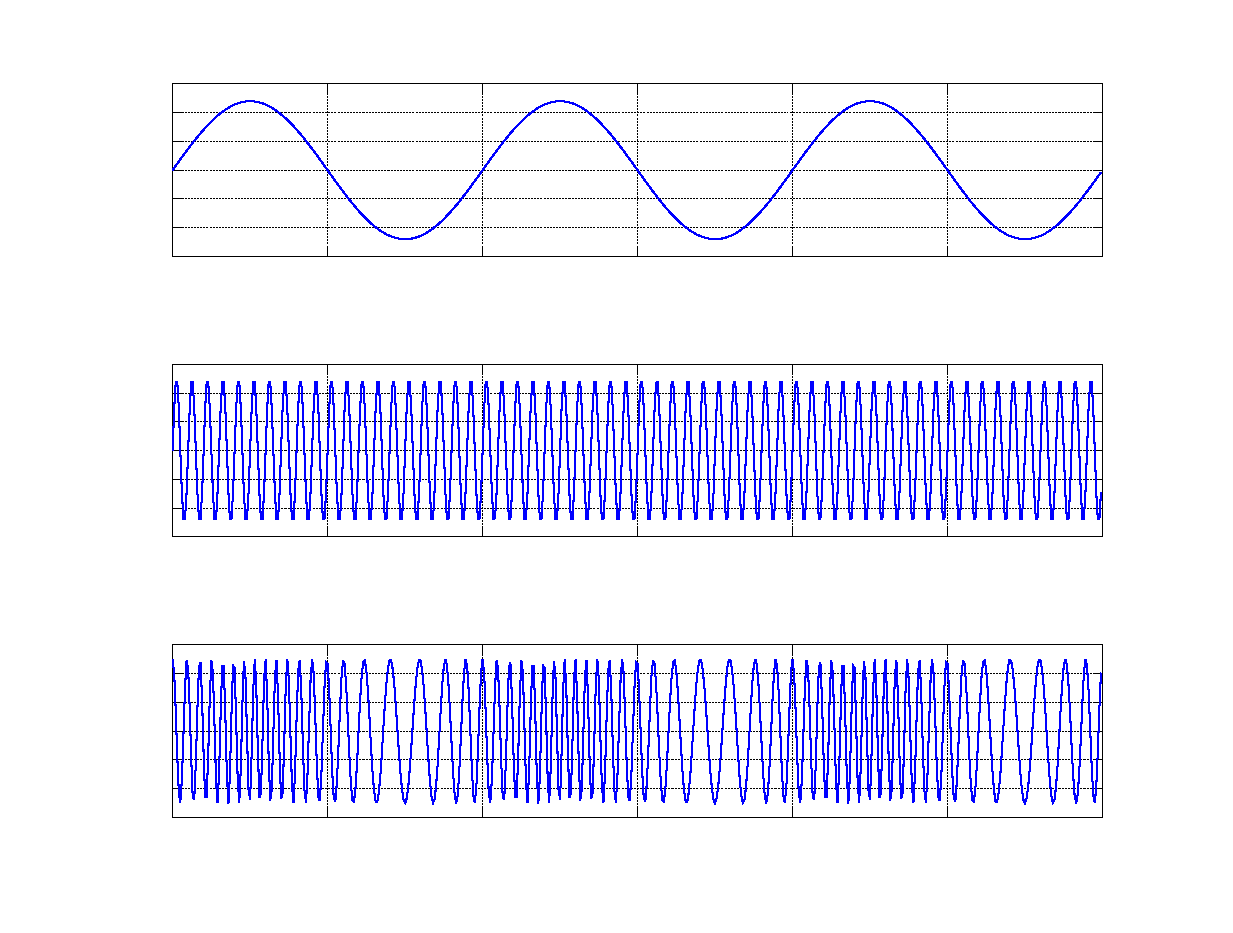
\includegraphics{fm}}%
    \gplfronttext
  \end{picture}%
\endgroup
$\end{large}}
  \caption{Frequenzmodulation}
  \label{fig:fm}
\end{figure}
Die Frequenzmodulation verändert die Frequenz des Trägersignals linear zur Amplitude des Nachrichtensignals.
Eine Implementierung einer solchen Modulation ist mit einem Voltage contolled oscillator (VCO) simpel zu realisieren. Die Demodulation erfolgt über einen Diskriminator, welcher auf vielfältige Art und Weise aufgebaut werden kann. Exemplarisch sei an dieser Stelle die Demodulation mit einem Phase locked loop (PLL) genannt. Eine PLL führt die Ausgangsfrequenz immer einer gegeben Eingangsfrequenz nach. Die Regeldifferenz aus diesen Größen lässt sich als Spannung abgreifen. Wird ein frequenzmoduliertes Signal als Soll-Signal vorgegeben so ist die genannte Regelspannung das demodulierte Nachrichtensignal.

\subsubsection{Amplitudenmodulation}
\begin{figure}[H]
\centering
  \scalebox{0.7}{\begin{large}$% GNUPLOT: LaTeX picture with Postscript
\begingroup
  \makeatletter
  \providecommand\color[2][]{%
    \GenericError{(gnuplot) \space\space\space\@spaces}{%
      Package color not loaded in conjunction with
      terminal option `colourtext'%
    }{See the gnuplot documentation for explanation.%
    }{Either use 'blacktext' in gnuplot or load the package
      color.sty in LaTeX.}%
    \renewcommand\color[2][]{}%
  }%
  \providecommand\includegraphics[2][]{%
    \GenericError{(gnuplot) \space\space\space\@spaces}{%
      Package graphicx or graphics not loaded%
    }{See the gnuplot documentation for explanation.%
    }{The gnuplot epslatex terminal needs graphicx.sty or graphics.sty.}%
    \renewcommand\includegraphics[2][]{}%
  }%
  \providecommand\rotatebox[2]{#2}%
  \@ifundefined{ifGPcolor}{%
    \newif\ifGPcolor
    \GPcolorfalse
  }{}%
  \@ifundefined{ifGPblacktext}{%
    \newif\ifGPblacktext
    \GPblacktexttrue
  }{}%
  % define a \g@addto@macro without @ in the name:
  \let\gplgaddtomacro\g@addto@macro
  % define empty templates for all commands taking text:
  \gdef\gplbacktext{}%
  \gdef\gplfronttext{}%
  \makeatother
  \ifGPblacktext
    % no textcolor at all
    \def\colorrgb#1{}%
    \def\colorgray#1{}%
  \else
    % gray or color?
    \ifGPcolor
      \def\colorrgb#1{\color[rgb]{#1}}%
      \def\colorgray#1{\color[gray]{#1}}%
      \expandafter\def\csname LTw\endcsname{\color{white}}%
      \expandafter\def\csname LTb\endcsname{\color{black}}%
      \expandafter\def\csname LTa\endcsname{\color{black}}%
      \expandafter\def\csname LT0\endcsname{\color[rgb]{1,0,0}}%
      \expandafter\def\csname LT1\endcsname{\color[rgb]{0,1,0}}%
      \expandafter\def\csname LT2\endcsname{\color[rgb]{0,0,1}}%
      \expandafter\def\csname LT3\endcsname{\color[rgb]{1,0,1}}%
      \expandafter\def\csname LT4\endcsname{\color[rgb]{0,1,1}}%
      \expandafter\def\csname LT5\endcsname{\color[rgb]{1,1,0}}%
      \expandafter\def\csname LT6\endcsname{\color[rgb]{0,0,0}}%
      \expandafter\def\csname LT7\endcsname{\color[rgb]{1,0.3,0}}%
      \expandafter\def\csname LT8\endcsname{\color[rgb]{0.5,0.5,0.5}}%
    \else
      % gray
      \def\colorrgb#1{\color{black}}%
      \def\colorgray#1{\color[gray]{#1}}%
      \expandafter\def\csname LTw\endcsname{\color{white}}%
      \expandafter\def\csname LTb\endcsname{\color{black}}%
      \expandafter\def\csname LTa\endcsname{\color{black}}%
      \expandafter\def\csname LT0\endcsname{\color{black}}%
      \expandafter\def\csname LT1\endcsname{\color{black}}%
      \expandafter\def\csname LT2\endcsname{\color{black}}%
      \expandafter\def\csname LT3\endcsname{\color{black}}%
      \expandafter\def\csname LT4\endcsname{\color{black}}%
      \expandafter\def\csname LT5\endcsname{\color{black}}%
      \expandafter\def\csname LT6\endcsname{\color{black}}%
      \expandafter\def\csname LT7\endcsname{\color{black}}%
      \expandafter\def\csname LT8\endcsname{\color{black}}%
    \fi
  \fi
    \setlength{\unitlength}{0.0500bp}%
    \ifx\gptboxheight\undefined%
      \newlength{\gptboxheight}%
      \newlength{\gptboxwidth}%
      \newsavebox{\gptboxtext}%
    \fi%
    \setlength{\fboxrule}{0.5pt}%
    \setlength{\fboxsep}{1pt}%
\begin{picture}(11520.00,8640.00)%
    \gplgaddtomacro\gplbacktext{%
      \colorrgb{0.00,0.00,0.00}%
      \put(1377,6335){\makebox(0,0)[r]{\strut{}-15}}%
      \colorrgb{0.00,0.00,0.00}%
      \put(1377,6611){\makebox(0,0)[r]{\strut{}-10}}%
      \colorrgb{0.00,0.00,0.00}%
      \put(1377,6887){\makebox(0,0)[r]{\strut{}-5}}%
      \colorrgb{0.00,0.00,0.00}%
      \put(1377,7163){\makebox(0,0)[r]{\strut{}0}}%
      \colorrgb{0.00,0.00,0.00}%
      \put(1377,7439){\makebox(0,0)[r]{\strut{}5}}%
      \colorrgb{0.00,0.00,0.00}%
      \put(1377,7715){\makebox(0,0)[r]{\strut{}10}}%
      \colorrgb{0.00,0.00,0.00}%
      \put(1377,7991){\makebox(0,0)[r]{\strut{}15}}%
      \colorrgb{0.00,0.00,0.00}%
      \put(1497,6135){\makebox(0,0){\strut{}0}}%
      \colorrgb{0.00,0.00,0.00}%
      \put(2985,6135){\makebox(0,0){\strut{}0.01}}%
      \colorrgb{0.00,0.00,0.00}%
      \put(4473,6135){\makebox(0,0){\strut{}0.02}}%
      \colorrgb{0.00,0.00,0.00}%
      \put(5961,6135){\makebox(0,0){\strut{}0.03}}%
      \colorrgb{0.00,0.00,0.00}%
      \put(7448,6135){\makebox(0,0){\strut{}0.04}}%
      \colorrgb{0.00,0.00,0.00}%
      \put(8936,6135){\makebox(0,0){\strut{}0.05}}%
      \colorrgb{0.00,0.00,0.00}%
      \put(10424,6135){\makebox(0,0){\strut{}0.06}}%
    }%
    \gplgaddtomacro\gplfronttext{%
      \colorrgb{0.00,0.00,0.00}%
      \put(797,7163){\rotatebox{90}{\makebox(0,0){\strut{}u_m/V}}}%
      \colorrgb{0.00,0.00,0.00}%
      \put(5960,5835){\makebox(0,0){\strut{}t/s}}%
      \colorrgb{0.00,0.00,0.00}%
      \put(5960,8191){\makebox(0,0){\strut{}Nachrichtensignal}}%
    }%
    \gplgaddtomacro\gplbacktext{%
      \colorrgb{0.00,0.00,0.00}%
      \put(1377,3643){\makebox(0,0)[r]{\strut{}-6}}%
      \colorrgb{0.00,0.00,0.00}%
      \put(1377,3919){\makebox(0,0)[r]{\strut{}-4}}%
      \colorrgb{0.00,0.00,0.00}%
      \put(1377,4195){\makebox(0,0)[r]{\strut{}-2}}%
      \colorrgb{0.00,0.00,0.00}%
      \put(1377,4471){\makebox(0,0)[r]{\strut{}0}}%
      \colorrgb{0.00,0.00,0.00}%
      \put(1377,4746){\makebox(0,0)[r]{\strut{}2}}%
      \colorrgb{0.00,0.00,0.00}%
      \put(1377,5022){\makebox(0,0)[r]{\strut{}4}}%
      \colorrgb{0.00,0.00,0.00}%
      \put(1377,5298){\makebox(0,0)[r]{\strut{}6}}%
      \colorrgb{0.00,0.00,0.00}%
      \put(1497,3443){\makebox(0,0){\strut{}0}}%
      \colorrgb{0.00,0.00,0.00}%
      \put(2985,3443){\makebox(0,0){\strut{}0.01}}%
      \colorrgb{0.00,0.00,0.00}%
      \put(4473,3443){\makebox(0,0){\strut{}0.02}}%
      \colorrgb{0.00,0.00,0.00}%
      \put(5961,3443){\makebox(0,0){\strut{}0.03}}%
      \colorrgb{0.00,0.00,0.00}%
      \put(7448,3443){\makebox(0,0){\strut{}0.04}}%
      \colorrgb{0.00,0.00,0.00}%
      \put(8936,3443){\makebox(0,0){\strut{}0.05}}%
      \colorrgb{0.00,0.00,0.00}%
      \put(10424,3443){\makebox(0,0){\strut{}0.06}}%
    }%
    \gplgaddtomacro\gplfronttext{%
      \colorrgb{0.00,0.00,0.00}%
      \put(917,4470){\rotatebox{90}{\makebox(0,0){\strut{}u_c/V}}}%
      \colorrgb{0.00,0.00,0.00}%
      \put(5960,3143){\makebox(0,0){\strut{}t/s}}%
      \colorrgb{0.00,0.00,0.00}%
      \put(5960,5498){\makebox(0,0){\strut{}Trägersignal}}%
    }%
    \gplgaddtomacro\gplbacktext{%
      \colorrgb{0.00,0.00,0.00}%
      \put(1377,950){\makebox(0,0)[r]{\strut{}-30}}%
      \colorrgb{0.00,0.00,0.00}%
      \put(1377,1226){\makebox(0,0)[r]{\strut{}-20}}%
      \colorrgb{0.00,0.00,0.00}%
      \put(1377,1502){\makebox(0,0)[r]{\strut{}-10}}%
      \colorrgb{0.00,0.00,0.00}%
      \put(1377,1778){\makebox(0,0)[r]{\strut{}0}}%
      \colorrgb{0.00,0.00,0.00}%
      \put(1377,2054){\makebox(0,0)[r]{\strut{}10}}%
      \colorrgb{0.00,0.00,0.00}%
      \put(1377,2330){\makebox(0,0)[r]{\strut{}20}}%
      \colorrgb{0.00,0.00,0.00}%
      \put(1377,2606){\makebox(0,0)[r]{\strut{}30}}%
      \colorrgb{0.00,0.00,0.00}%
      \put(1497,750){\makebox(0,0){\strut{}0}}%
      \colorrgb{0.00,0.00,0.00}%
      \put(2985,750){\makebox(0,0){\strut{}0.01}}%
      \colorrgb{0.00,0.00,0.00}%
      \put(4473,750){\makebox(0,0){\strut{}0.02}}%
      \colorrgb{0.00,0.00,0.00}%
      \put(5961,750){\makebox(0,0){\strut{}0.03}}%
      \colorrgb{0.00,0.00,0.00}%
      \put(7448,750){\makebox(0,0){\strut{}0.04}}%
      \colorrgb{0.00,0.00,0.00}%
      \put(8936,750){\makebox(0,0){\strut{}0.05}}%
      \colorrgb{0.00,0.00,0.00}%
      \put(10424,750){\makebox(0,0){\strut{}0.06}}%
    }%
    \gplgaddtomacro\gplfronttext{%
      \colorrgb{0.00,0.00,0.00}%
      \put(797,1778){\rotatebox{90}{\makebox(0,0){\strut{}u_{am}/V}}}%
      \colorrgb{0.00,0.00,0.00}%
      \put(5960,450){\makebox(0,0){\strut{}t/s}}%
      \colorrgb{0.00,0.00,0.00}%
      \put(5960,2806){\makebox(0,0){\strut{}Amplitudenmoduliertes Signal}}%
    }%
    \gplbacktext
    \put(0,0){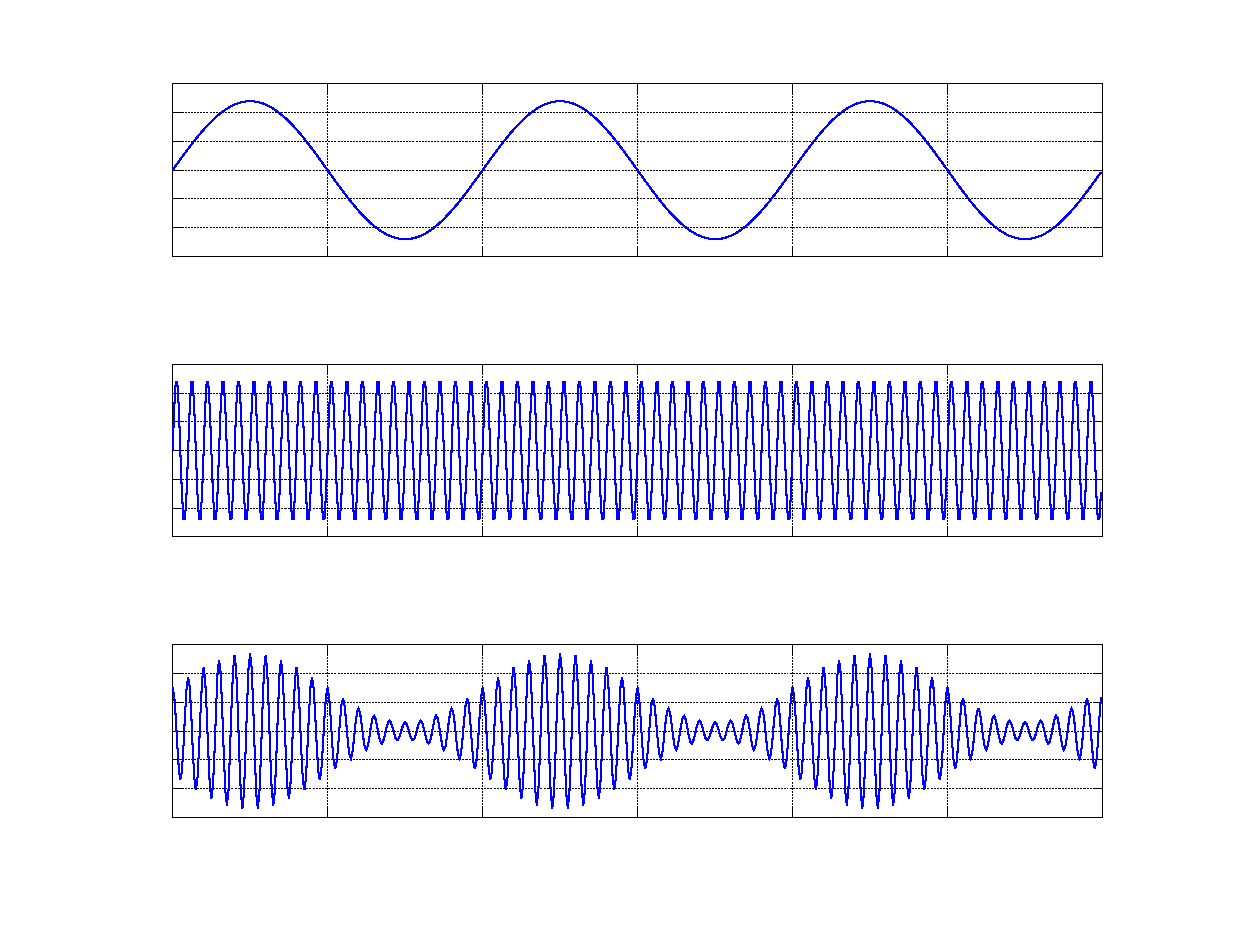
\includegraphics{am}}%
    \gplfronttext
  \end{picture}%
\endgroup
$\end{large}}
  \caption{Amplitudenmodulation}
  \label{fig:am}
\end{figure}
Die Amplitudenmodulation verändert die Amplitude des Trägersignals proportional zum Nachrichtensignal.
Eine Amplitudenmodulation lässt sich durch Anwendung eines 4 Quadranten-Mischers unkompliziert implementieren. Zur Modulation werden lediglich ein Trägersignal, welches eine vielfache Frequenz des Nachrichtensignals haben muss, und das Nachrichtensignal multiplizert. Anschließend werden unerwünsche Mischprodukte herausgefiltert. Die Demodulation erfolgt über einen Tiefpass, dessen Grenzfrequenz weit unter der gewählten Trägerfrequenz liegt.
Da bei dieser Modulation die Information genauso wie bei der direkten Übertragung in der Amplitude liegt, entstehen wieder die gleichen Probleme durch die Dämpfung des Lichtwellenleiters.

\subsection{Digitale Übertragungsarten}
\subsubsection{Pulsweitenmodulation}
\begin{figure}[H]
\centering
  \scalebox{0.7}{\begin{large}
  $% GNUPLOT: LaTeX picture with Postscript
\begingroup
  \makeatletter
  \providecommand\color[2][]{%
    \GenericError{(gnuplot) \space\space\space\@spaces}{%
      Package color not loaded in conjunction with
      terminal option `colourtext'%
    }{See the gnuplot documentation for explanation.%
    }{Either use 'blacktext' in gnuplot or load the package
      color.sty in LaTeX.}%
    \renewcommand\color[2][]{}%
  }%
  \providecommand\includegraphics[2][]{%
    \GenericError{(gnuplot) \space\space\space\@spaces}{%
      Package graphicx or graphics not loaded%
    }{See the gnuplot documentation for explanation.%
    }{The gnuplot epslatex terminal needs graphicx.sty or graphics.sty.}%
    \renewcommand\includegraphics[2][]{}%
  }%
  \providecommand\rotatebox[2]{#2}%
  \@ifundefined{ifGPcolor}{%
    \newif\ifGPcolor
    \GPcolorfalse
  }{}%
  \@ifundefined{ifGPblacktext}{%
    \newif\ifGPblacktext
    \GPblacktexttrue
  }{}%
  % define a \g@addto@macro without @ in the name:
  \let\gplgaddtomacro\g@addto@macro
  % define empty templates for all commands taking text:
  \gdef\gplbacktext{}%
  \gdef\gplfronttext{}%
  \makeatother
  \ifGPblacktext
    % no textcolor at all
    \def\colorrgb#1{}%
    \def\colorgray#1{}%
  \else
    % gray or color?
    \ifGPcolor
      \def\colorrgb#1{\color[rgb]{#1}}%
      \def\colorgray#1{\color[gray]{#1}}%
      \expandafter\def\csname LTw\endcsname{\color{white}}%
      \expandafter\def\csname LTb\endcsname{\color{black}}%
      \expandafter\def\csname LTa\endcsname{\color{black}}%
      \expandafter\def\csname LT0\endcsname{\color[rgb]{1,0,0}}%
      \expandafter\def\csname LT1\endcsname{\color[rgb]{0,1,0}}%
      \expandafter\def\csname LT2\endcsname{\color[rgb]{0,0,1}}%
      \expandafter\def\csname LT3\endcsname{\color[rgb]{1,0,1}}%
      \expandafter\def\csname LT4\endcsname{\color[rgb]{0,1,1}}%
      \expandafter\def\csname LT5\endcsname{\color[rgb]{1,1,0}}%
      \expandafter\def\csname LT6\endcsname{\color[rgb]{0,0,0}}%
      \expandafter\def\csname LT7\endcsname{\color[rgb]{1,0.3,0}}%
      \expandafter\def\csname LT8\endcsname{\color[rgb]{0.5,0.5,0.5}}%
    \else
      % gray
      \def\colorrgb#1{\color{black}}%
      \def\colorgray#1{\color[gray]{#1}}%
      \expandafter\def\csname LTw\endcsname{\color{white}}%
      \expandafter\def\csname LTb\endcsname{\color{black}}%
      \expandafter\def\csname LTa\endcsname{\color{black}}%
      \expandafter\def\csname LT0\endcsname{\color{black}}%
      \expandafter\def\csname LT1\endcsname{\color{black}}%
      \expandafter\def\csname LT2\endcsname{\color{black}}%
      \expandafter\def\csname LT3\endcsname{\color{black}}%
      \expandafter\def\csname LT4\endcsname{\color{black}}%
      \expandafter\def\csname LT5\endcsname{\color{black}}%
      \expandafter\def\csname LT6\endcsname{\color{black}}%
      \expandafter\def\csname LT7\endcsname{\color{black}}%
      \expandafter\def\csname LT8\endcsname{\color{black}}%
    \fi
  \fi
    \setlength{\unitlength}{0.0500bp}%
    \ifx\gptboxheight\undefined%
      \newlength{\gptboxheight}%
      \newlength{\gptboxwidth}%
      \newsavebox{\gptboxtext}%
    \fi%
    \setlength{\fboxrule}{0.5pt}%
    \setlength{\fboxsep}{1pt}%
\begin{picture}(11520.00,8640.00)%
    \gplgaddtomacro\gplbacktext{%
      \colorrgb{0.00,0.00,0.00}%
      \put(1377,6335){\makebox(0,0)[r]{\strut{}-15}}%
      \colorrgb{0.00,0.00,0.00}%
      \put(1377,6611){\makebox(0,0)[r]{\strut{}-10}}%
      \colorrgb{0.00,0.00,0.00}%
      \put(1377,6887){\makebox(0,0)[r]{\strut{}-5}}%
      \colorrgb{0.00,0.00,0.00}%
      \put(1377,7163){\makebox(0,0)[r]{\strut{}0}}%
      \colorrgb{0.00,0.00,0.00}%
      \put(1377,7439){\makebox(0,0)[r]{\strut{}5}}%
      \colorrgb{0.00,0.00,0.00}%
      \put(1377,7715){\makebox(0,0)[r]{\strut{}10}}%
      \colorrgb{0.00,0.00,0.00}%
      \put(1377,7991){\makebox(0,0)[r]{\strut{}15}}%
      \colorrgb{0.00,0.00,0.00}%
      \put(1497,6135){\makebox(0,0){\strut{}0}}%
      \colorrgb{0.00,0.00,0.00}%
      \put(2985,6135){\makebox(0,0){\strut{}0.01}}%
      \colorrgb{0.00,0.00,0.00}%
      \put(4473,6135){\makebox(0,0){\strut{}0.02}}%
      \colorrgb{0.00,0.00,0.00}%
      \put(5961,6135){\makebox(0,0){\strut{}0.03}}%
      \colorrgb{0.00,0.00,0.00}%
      \put(7448,6135){\makebox(0,0){\strut{}0.04}}%
      \colorrgb{0.00,0.00,0.00}%
      \put(8936,6135){\makebox(0,0){\strut{}0.05}}%
      \colorrgb{0.00,0.00,0.00}%
      \put(10424,6135){\makebox(0,0){\strut{}0.06}}%
    }%
    \gplgaddtomacro\gplfronttext{%
      \colorrgb{0.00,0.00,0.00}%
      \put(797,7163){\rotatebox{90}{\makebox(0,0){\strut{}u_m/V}}}%
      \colorrgb{0.00,0.00,0.00}%
      \put(5960,5835){\makebox(0,0){\strut{}t/s}}%
      \colorrgb{0.00,0.00,0.00}%
      \put(5960,8191){\makebox(0,0){\strut{}Nachrichtensignal}}%
    }%
    \gplgaddtomacro\gplbacktext{%
      \colorrgb{0.00,0.00,0.00}%
      \put(1377,3643){\makebox(0,0)[r]{\strut{}-15}}%
      \colorrgb{0.00,0.00,0.00}%
      \put(1377,3919){\makebox(0,0)[r]{\strut{}-10}}%
      \colorrgb{0.00,0.00,0.00}%
      \put(1377,4195){\makebox(0,0)[r]{\strut{}-5}}%
      \colorrgb{0.00,0.00,0.00}%
      \put(1377,4471){\makebox(0,0)[r]{\strut{}0}}%
      \colorrgb{0.00,0.00,0.00}%
      \put(1377,4746){\makebox(0,0)[r]{\strut{}5}}%
      \colorrgb{0.00,0.00,0.00}%
      \put(1377,5022){\makebox(0,0)[r]{\strut{}10}}%
      \colorrgb{0.00,0.00,0.00}%
      \put(1377,5298){\makebox(0,0)[r]{\strut{}15}}%
      \colorrgb{0.00,0.00,0.00}%
      \put(1497,3443){\makebox(0,0){\strut{}0}}%
      \colorrgb{0.00,0.00,0.00}%
      \put(2985,3443){\makebox(0,0){\strut{}0.01}}%
      \colorrgb{0.00,0.00,0.00}%
      \put(4473,3443){\makebox(0,0){\strut{}0.02}}%
      \colorrgb{0.00,0.00,0.00}%
      \put(5961,3443){\makebox(0,0){\strut{}0.03}}%
      \colorrgb{0.00,0.00,0.00}%
      \put(7448,3443){\makebox(0,0){\strut{}0.04}}%
      \colorrgb{0.00,0.00,0.00}%
      \put(8936,3443){\makebox(0,0){\strut{}0.05}}%
      \colorrgb{0.00,0.00,0.00}%
      \put(10424,3443){\makebox(0,0){\strut{}0.06}}%
    }%
    \gplgaddtomacro\gplfronttext{%
      \colorrgb{0.00,0.00,0.00}%
      \put(797,4470){\rotatebox{90}{\makebox(0,0){\strut{}u_c/V}}}%
      \colorrgb{0.00,0.00,0.00}%
      \put(5960,3143){\makebox(0,0){\strut{}t/s}}%
      \colorrgb{0.00,0.00,0.00}%
      \put(5960,5498){\makebox(0,0){\strut{}Trägersignal}}%
    }%
    \gplgaddtomacro\gplbacktext{%
      \colorrgb{0.00,0.00,0.00}%
      \put(1377,950){\makebox(0,0)[r]{\strut{}-0.5}}%
      \colorrgb{0.00,0.00,0.00}%
      \put(1377,1344){\makebox(0,0)[r]{\strut{}0}}%
      \colorrgb{0.00,0.00,0.00}%
      \put(1377,1739){\makebox(0,0)[r]{\strut{}0.5}}%
      \colorrgb{0.00,0.00,0.00}%
      \put(1377,2133){\makebox(0,0)[r]{\strut{}1}}%
      \colorrgb{0.00,0.00,0.00}%
      \put(1377,2527){\makebox(0,0)[r]{\strut{}1.5}}%
      \colorrgb{0.00,0.00,0.00}%
      \put(1497,750){\makebox(0,0){\strut{}0}}%
      \colorrgb{0.00,0.00,0.00}%
      \put(2985,750){\makebox(0,0){\strut{}0.01}}%
      \colorrgb{0.00,0.00,0.00}%
      \put(4473,750){\makebox(0,0){\strut{}0.02}}%
      \colorrgb{0.00,0.00,0.00}%
      \put(5961,750){\makebox(0,0){\strut{}0.03}}%
      \colorrgb{0.00,0.00,0.00}%
      \put(7448,750){\makebox(0,0){\strut{}0.04}}%
      \colorrgb{0.00,0.00,0.00}%
      \put(8936,750){\makebox(0,0){\strut{}0.05}}%
      \colorrgb{0.00,0.00,0.00}%
      \put(10424,750){\makebox(0,0){\strut{}0.06}}%
    }%
    \gplgaddtomacro\gplfronttext{%
      \colorrgb{0.00,0.00,0.00}%
      \put(677,1778){\rotatebox{90}{\makebox(0,0){\strut{}u_{pwm}/V}}}%
      \colorrgb{0.00,0.00,0.00}%
      \put(5960,450){\makebox(0,0){\strut{}t/s}}%
      \colorrgb{0.00,0.00,0.00}%
      \put(5960,2806){\makebox(0,0){\strut{}Pulsweitenmoduliertes Signal}}%
    }%
    \gplbacktext
    \put(0,0){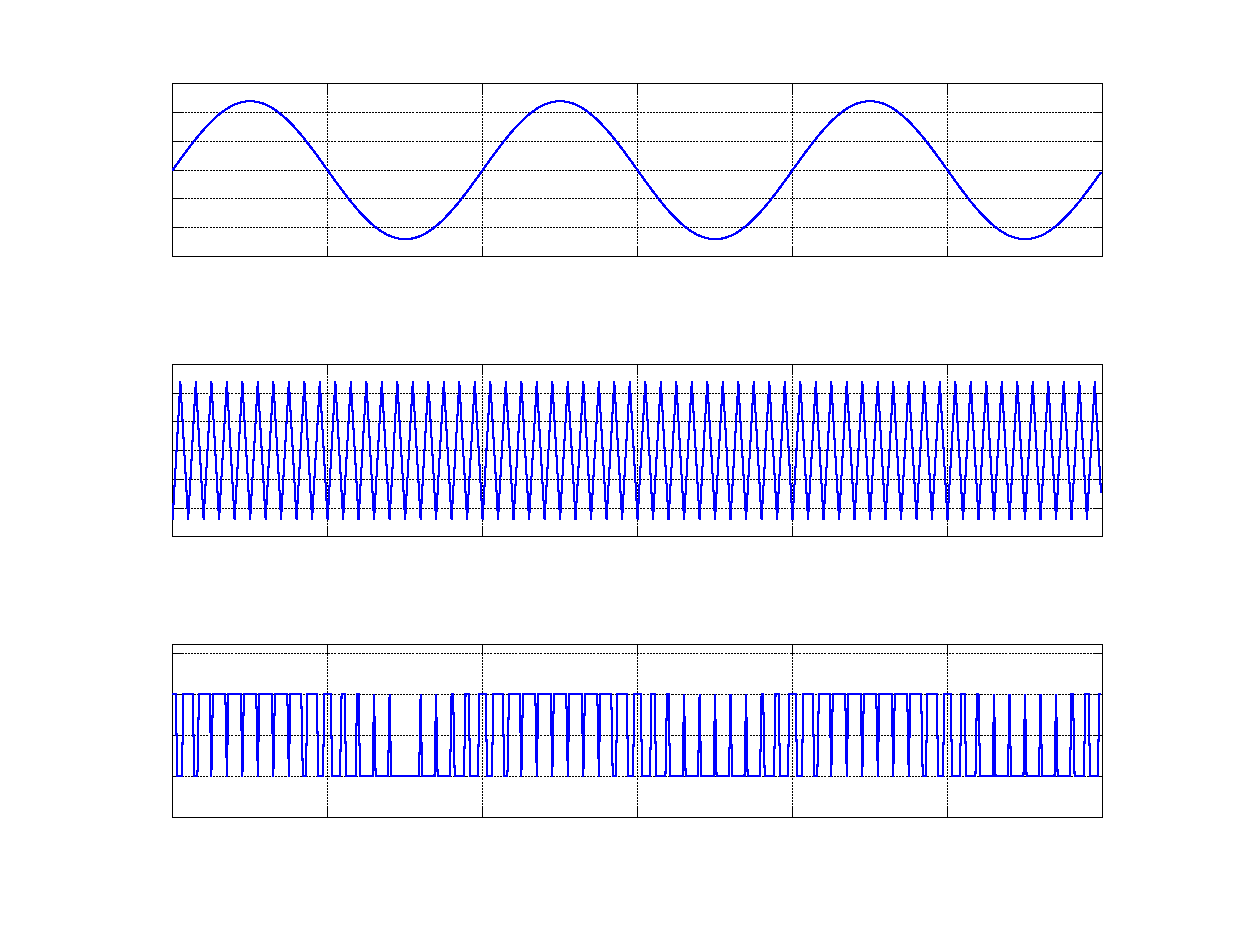
\includegraphics{pwm}}%
    \gplfronttext
  \end{picture}%
\endgroup
$
  \end{large}}
  \caption{Pulsweitenmodulation}
  \label{fig:pwm}
\end{figure}
Die Pulsweitenmodulation moduliert, ähnlich wie die Frequenzmodulation, das Nachrichtensignal im Zeitbereich. 
Die essentiellen Unterschiede liegen zum Einen darin, dass die PWM ein digitales Übertragungsverfahren ist und demnach nur 2 Zustände kennt, und zum Anderen, dass das Nachrichtensignal nicht direkt in der Frequenz sondern in der Pulsweite des Trägersignals kodiert wird. Die Synthese einer Pulsweitenmodulation kann durch den Vergleich des Nachrichtensignals mit einer Dreiecksspannung erfolgen. Hierbei ist darauf zu achten, dass die Dreieckspannung, welche als Träger verwendet wird, eine vielfache Frequenz des Nachrichtensignals aufweist. Die Demodulation eines pulsweitenmodulierten Signals erfolgt durch einen Tiefpass, welcher ledglich das Nachrichtensignal im Passband hat. 




\subsection{Wahl des Übertragungsverfahren}
Eine unmodulierte Übertragung ist aufgrund der Leitungsdämpfung ausgeschlossen. Entsprechend kommt folgender genereller Systemaufbau in Frage.
\begin{figure}[H]
\centering
  \input{prinzip.pdf_tex}
  \caption{Genereller Systemaufbau}
  \label{fig:psystem}
\end{figure}
Die Evaluation der drei verbliebenen Varianten liefert die Pulsweitenmodulation (PWM) als optimales Ergebnis:
Im Gegensatz zu allen analogen Übertragungsverfahren lässt sich die PWM durch Übersteuerung des Eingangsverstärkers der Empfängereinheit sehr einfach rekonstruieren und ist demnach unempfindlich gegenüber Variationen der Dämpfung der Leitungslänge. Darüber hinaus ist die Synthese sowie Demodulation einer PWM mit einfachen Mitteln umzusetzen.\\
Neben den grundlegenden Aufgaben des Systems, wie Modulation und Demodulation, müssen noch weitere Komponenten wie eine Endstufe und eine Schutzschaltung gegenüber der Hochspannung im System verbaut werden. 
Aus allen vorangegangen Überlegungen geht folgender Systemaufbau hervor: 
\begin{figure}[H]
  \centering
  \input{systemaufbau.pdf_tex}
  \caption{Systemaufbau}
  \label{fig:system}
\end{figure}

\subsection{Pulsweitenmodulation - Theorie}
\label{sec:pwmTheory}
Im wesentlichen basiert die Funktionsweise einer PWM auf der Variation des Tastverhältnisses einer Rechteckspannung. Durch die Änderung des Tastverhältnis wird der Effektivwert der Rechteckspannung verändert, dieser berechnet sich wie folgt:\\
\begin{equation}
 U_{eff} = \sqrt{\frac{1}{T}\cdot\int\limits_{0}^T u(t)^2 dt}
\end{equation}
Offensichtlich ist der Effektivwert von dem Integral der Kurve über eine Periode, also der Fläche unter der Kurve, abhängig. Diese Fläche wird wie bereits beschrieben über das Tastverhältnis bestimmt. So kann jede Perdiode des Rechteckssignals als ein Abstastwert des Nachrichtensignals interpretiert werden. Dieses Integral ist beispielhaft für 2 Perioden eines Sinussignals in Abbildung \ref{fig:pwmArea} dargestellt. Aufgrund dieser Abtastung ist es wichtig, dass zur optimalen Rekonstruktion das 50 Hz Eingangssignal um ein Vielfaches abgetastet wird. Für diese Anwendung wurde eine 200-fache Überabtastung von $f_A=10kHz$ gewählt.
\begin{figure}[H]
  \centering
   \scalebox{0.6}{\begin{Large}
   % GNUPLOT: LaTeX picture with Postscript
\begingroup
  \makeatletter
  \providecommand\color[2][]{%
    \GenericError{(gnuplot) \space\space\space\@spaces}{%
      Package color not loaded in conjunction with
      terminal option `colourtext'%
    }{See the gnuplot documentation for explanation.%
    }{Either use 'blacktext' in gnuplot or load the package
      color.sty in LaTeX.}%
    \renewcommand\color[2][]{}%
  }%
  \providecommand\includegraphics[2][]{%
    \GenericError{(gnuplot) \space\space\space\@spaces}{%
      Package graphicx or graphics not loaded%
    }{See the gnuplot documentation for explanation.%
    }{The gnuplot epslatex terminal needs graphicx.sty or graphics.sty.}%
    \renewcommand\includegraphics[2][]{}%
  }%
  \providecommand\rotatebox[2]{#2}%
  \@ifundefined{ifGPcolor}{%
    \newif\ifGPcolor
    \GPcolorfalse
  }{}%
  \@ifundefined{ifGPblacktext}{%
    \newif\ifGPblacktext
    \GPblacktexttrue
  }{}%
  % define a \g@addto@macro without @ in the name:
  \let\gplgaddtomacro\g@addto@macro
  % define empty templates for all commands taking text:
  \gdef\gplbacktext{}%
  \gdef\gplfronttext{}%
  \makeatother
  \ifGPblacktext
    % no textcolor at all
    \def\colorrgb#1{}%
    \def\colorgray#1{}%
  \else
    % gray or color?
    \ifGPcolor
      \def\colorrgb#1{\color[rgb]{#1}}%
      \def\colorgray#1{\color[gray]{#1}}%
      \expandafter\def\csname LTw\endcsname{\color{white}}%
      \expandafter\def\csname LTb\endcsname{\color{black}}%
      \expandafter\def\csname LTa\endcsname{\color{black}}%
      \expandafter\def\csname LT0\endcsname{\color[rgb]{1,0,0}}%
      \expandafter\def\csname LT1\endcsname{\color[rgb]{0,1,0}}%
      \expandafter\def\csname LT2\endcsname{\color[rgb]{0,0,1}}%
      \expandafter\def\csname LT3\endcsname{\color[rgb]{1,0,1}}%
      \expandafter\def\csname LT4\endcsname{\color[rgb]{0,1,1}}%
      \expandafter\def\csname LT5\endcsname{\color[rgb]{1,1,0}}%
      \expandafter\def\csname LT6\endcsname{\color[rgb]{0,0,0}}%
      \expandafter\def\csname LT7\endcsname{\color[rgb]{1,0.3,0}}%
      \expandafter\def\csname LT8\endcsname{\color[rgb]{0.5,0.5,0.5}}%
    \else
      % gray
      \def\colorrgb#1{\color{black}}%
      \def\colorgray#1{\color[gray]{#1}}%
      \expandafter\def\csname LTw\endcsname{\color{white}}%
      \expandafter\def\csname LTb\endcsname{\color{black}}%
      \expandafter\def\csname LTa\endcsname{\color{black}}%
      \expandafter\def\csname LT0\endcsname{\color{black}}%
      \expandafter\def\csname LT1\endcsname{\color{black}}%
      \expandafter\def\csname LT2\endcsname{\color{black}}%
      \expandafter\def\csname LT3\endcsname{\color{black}}%
      \expandafter\def\csname LT4\endcsname{\color{black}}%
      \expandafter\def\csname LT5\endcsname{\color{black}}%
      \expandafter\def\csname LT6\endcsname{\color{black}}%
      \expandafter\def\csname LT7\endcsname{\color{black}}%
      \expandafter\def\csname LT8\endcsname{\color{black}}%
    \fi
  \fi
    \setlength{\unitlength}{0.0500bp}%
    \ifx\gptboxheight\undefined%
      \newlength{\gptboxheight}%
      \newlength{\gptboxwidth}%
      \newsavebox{\gptboxtext}%
    \fi%
    \setlength{\fboxrule}{0.5pt}%
    \setlength{\fboxsep}{1pt}%
\begin{picture}(11520.00,4320.00)%
    \gplgaddtomacro\gplbacktext{%
      \colorrgb{0.00,0.00,0.00}%
      \put(860,640){\makebox(0,0)[r]{\strut{}-0.5}}%
      \colorrgb{0.00,0.00,0.00}%
      \put(860,1397){\makebox(0,0)[r]{\strut{}0}}%
      \colorrgb{0.00,0.00,0.00}%
      \put(860,2154){\makebox(0,0)[r]{\strut{}0.5}}%
      \colorrgb{0.00,0.00,0.00}%
      \put(860,2911){\makebox(0,0)[r]{\strut{}1}}%
      \colorrgb{0.00,0.00,0.00}%
      \put(860,3668){\makebox(0,0)[r]{\strut{}1.5}}%
      \colorrgb{0.00,0.00,0.00}%
      \put(980,440){\makebox(0,0){\strut{}0}}%
      \colorrgb{0.00,0.00,0.00}%
      \put(2252,440){\makebox(0,0){\strut{}0.005}}%
      \colorrgb{0.00,0.00,0.00}%
      \put(3525,440){\makebox(0,0){\strut{}0.01}}%
      \colorrgb{0.00,0.00,0.00}%
      \put(4797,440){\makebox(0,0){\strut{}0.015}}%
      \colorrgb{0.00,0.00,0.00}%
      \put(6070,440){\makebox(0,0){\strut{}0.02}}%
      \colorrgb{0.00,0.00,0.00}%
      \put(7342,440){\makebox(0,0){\strut{}0.025}}%
      \colorrgb{0.00,0.00,0.00}%
      \put(8614,440){\makebox(0,0){\strut{}0.03}}%
      \colorrgb{0.00,0.00,0.00}%
      \put(9887,440){\makebox(0,0){\strut{}0.035}}%
      \colorrgb{0.00,0.00,0.00}%
      \put(11159,440){\makebox(0,0){\strut{}0.04}}%
    }%
    \gplgaddtomacro\gplfronttext{%
      \colorrgb{0.00,0.00,0.00}%
      \put(160,2229){\rotatebox{90}{\makebox(0,0){\strut{}u_{pwm}/V}}}%
      \colorrgb{0.00,0.00,0.00}%
      \put(6069,140){\makebox(0,0){\strut{}t/s}}%
      \colorrgb{0.00,0.00,0.00}%
      \put(6069,4019){\makebox(0,0){\strut{}Pulsweitenmoduliertes Signal}}%
    }%
    \gplbacktext
    \put(0,0){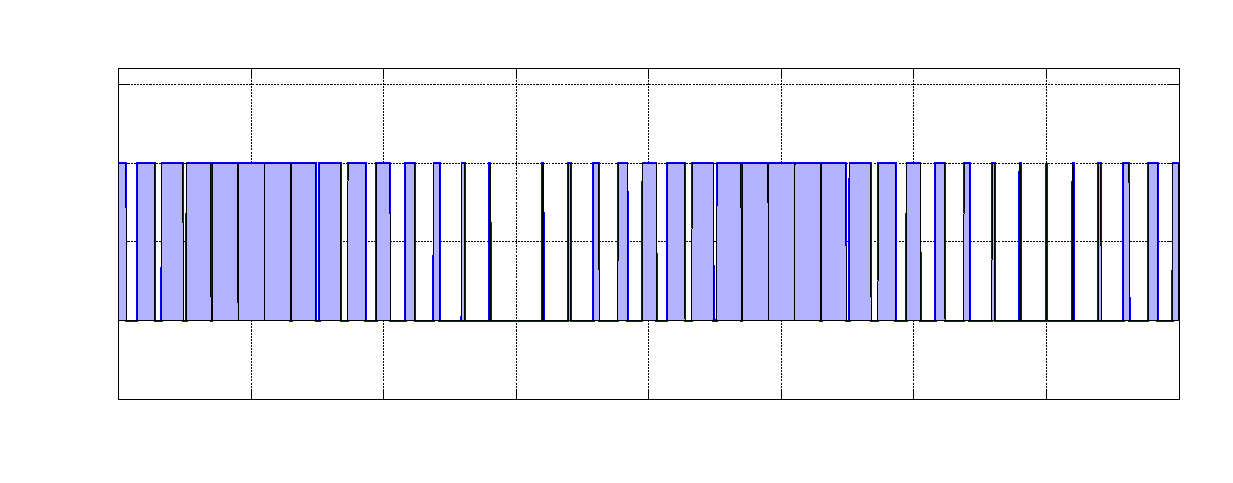
\includegraphics{pwmArea}}%
    \gplfronttext
  \end{picture}%
\endgroup

   \end{Large}}
   \caption{Pulsweitenmodulation Illustration}
  \label{fig:pwmArea}
\end{figure}

\newpage

\section{Projektstruktur}
Das Projekt wird in folgende Teilprobleme zerlegt. 
\begin{figure}[H]
\centering
  \scalebox{0.85}{
 \section{Projektstruktur}
Das Projekt wird in folgende Teilprobleme zerlegt. 
\begin{figure}[H]
\centering
  \scalebox{0.85}{
 \section{Projektstruktur}
Das Projekt wird in folgende Teilprobleme zerlegt. 
\begin{figure}[H]
\centering
  \scalebox{0.85}{
 \input{projektstruktur.pdf_tex}}
	\caption{Projektstruktur}
\end{figure}
Im Laufe der Projektarbeit wird jedes einzelne Teilproblem mit Komponententests validiert. Schlussendlich wird das Gesamtsystem getestet.}
	\caption{Projektstruktur}
\end{figure}
Im Laufe der Projektarbeit wird jedes einzelne Teilproblem mit Komponententests validiert. Schlussendlich wird das Gesamtsystem getestet.}
	\caption{Projektstruktur}
\end{figure}
Im Laufe der Projektarbeit wird jedes einzelne Teilproblem mit Komponententests validiert. Schlussendlich wird das Gesamtsystem getestet.
\section{Schaltungsentwurf - Sendeeinheit}
\subsection{Spannungsversorgung}
\begin{floatingfigure}[r]{6.5cm}
\centering
 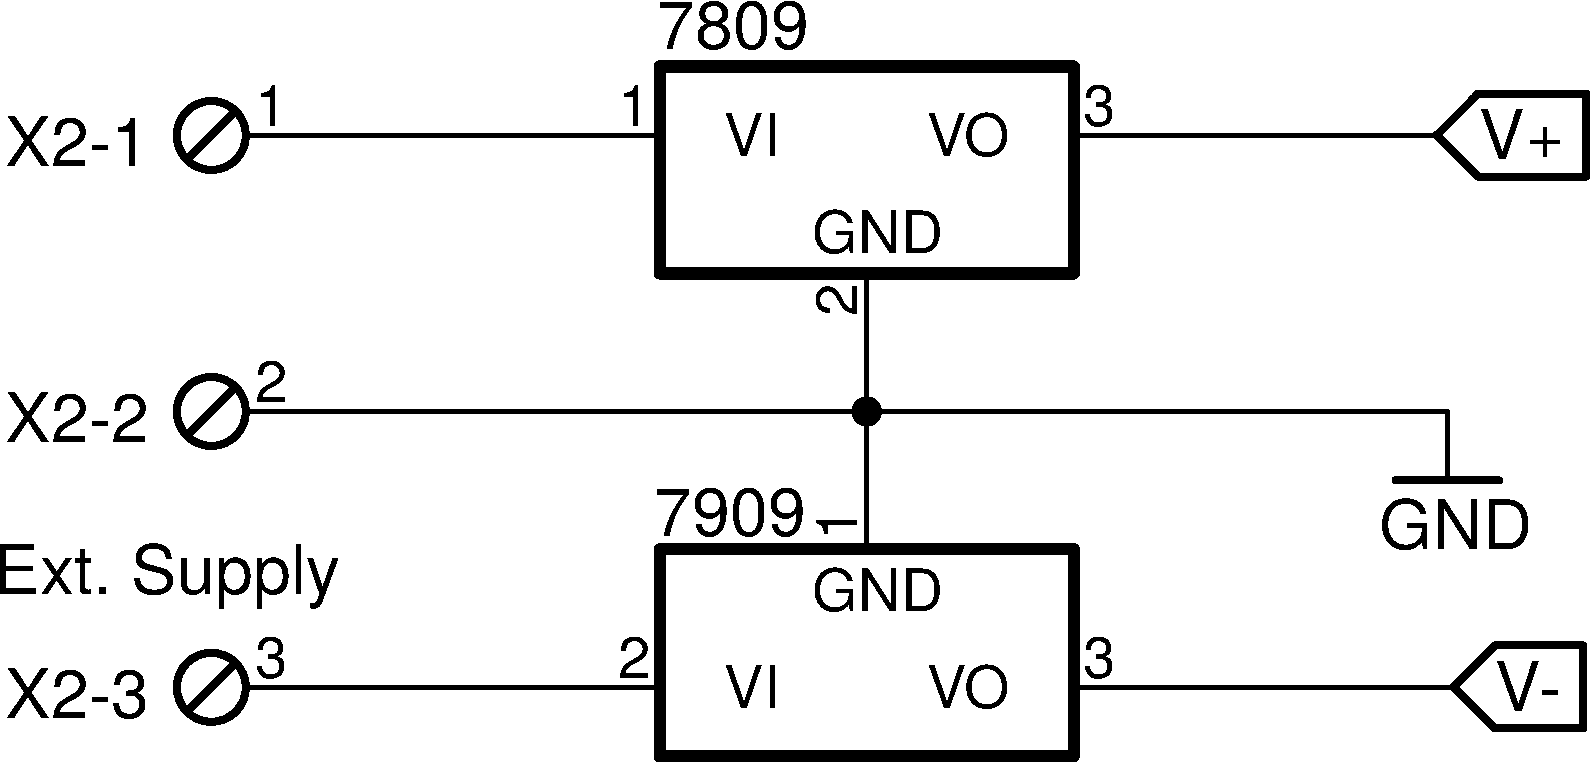
\includegraphics[width=6cm]{gfx/vcc.pdf}
\caption{Spannungsversorgung}
\label{fig:vcc}
\vspace{0.5cm}
\end{floatingfigure}
\noindent
Die Spannungsversorgung für die Sendeeinheit erfolgt zur galvanischen Trennung über Batterien. Aufgrund der hohen Stromaufnahme durch die Sendediode sowie der Status-LEDs ist eine interne Versorgung über 9V Blockbatterien nur bedingt möglich. Deswegen wird auf eine externe Versorgng über 12V Akkus zurückgegriffen. Damit die Schaltung dennoch bei allen Akkuspannungen zuverlässig und mit gleichen Ergebnissen arbeitet wird die Spannung intern auf 9V stabilisiert.
\subsection{Eingangsstufe}
\begin{figure}[H]
\centering
 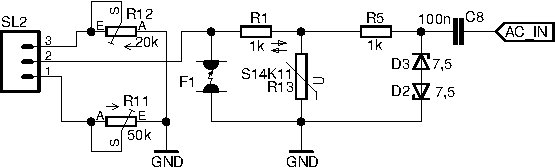
\includegraphics[scale=1]{gfx/eingangstufe.pdf}
 \caption{Kaskade}
	\label{kaskade} 
\end{figure}
Die Eingangsstufe der Sendeeinheit dient einerseits zur Einstellung der gewünschten Impedanz und andererseits der Schaltung der folgenden Komponenten.
Beiden Potentiometer ($R_{12}$ , $R_{13}$) werden durch einen Kippschalter an der Front des Geräts umgeschaltet. Die folgenden 3 Schaltungsteile, welche durch $1k\Omega$ Widerstände miteinander verbunden sind dienen dem Kurzschluss von Überspannungen. Der Gasableiter ist mit einer Druchbruchspannung von $60V$ gewählt, der Varistor S14K11 ist mit einer AC-Durchbruchspannung von $11V$ gewählt und die Zenerdioden mit einer Zenerspannung von $7,5V$ dimensioniert.\\
Diese Schaltungs-Topologie sorgt für einen zuverlässigen Schutz gegenüber Überspannungen. Die Zener-Dioden, schalten am schnellsten und sind entsprechend am nähesten zur zu schützenden Komponente verortet. Der Varistor spricht langsamer als die Zener-Dioden an, jedoch schneller als der Gasableiter. Die einzelnen Schutzbauteile sind der Verlustleistung und der Ansprechzeit nach absteigend in Richtung der folgenden Schaltungsteile angeordnet.

\begin{floatingfigure}[r]{6.5cm}
\input{impedanz2.pdf_tex}}
\caption{Spannungsversorgung}
\label{fig:vkkkcc}
\vspace{0.5cm}
\end{floatingfigure}
\noindent
egergsfgsreghtsrhdt


\subsection{Dreiecksgenerator}
\begin{figure}[H]
\centering
 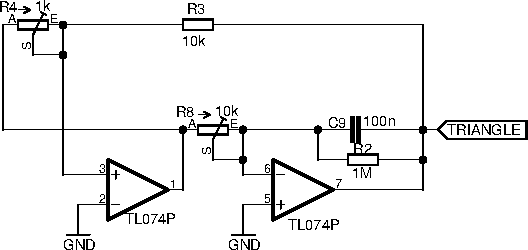
\includegraphics[scale=1]{gfx/triangle_generator.pdf}
 \caption{Miller Integrator}
	\label{triangle} 
\end{figure}
Für die Generierung eines Dreiecksignals wurde ein Miller-Integrator verwendet.
Die Grundlage für die Schaltung liegt in einer Applicationnote von TI\footnote{ Texas Instruments,Appnote 20, Seite 24, www.ti.com/lit/an/snoa621c/snoa621c.pdf}
Das Grundprinzip dieser Schaltung besteht aus einem Intergrator, welcher auf einen invertierenden Schmitt-Trigger rückgekoppelt ist.
Der linke Operationsverstärker bildet mit $R_4$ und $R_3$ den Schmitt-Trigger. Der Integrator besteht aus $R_8$,$C_1$ und dem rechten Operationsverstärker in Abbildung \ref{triangle}.
Frequenzbestimmend sind in dieser Schaltung alle Bauteile. Durch $R_4$ und $R_3$ werden die Schaltschwellen, und damit die Amplitude bestimmt. Diese berechnet sich wie folgt: 
\begin{equation}
U_H = \pm\frac{R_3}{R_4}\cdot V_{cc}
\end{equation}
Mit $R_8$ und $C_1$ wird die Flankensteilheit($k$) in $\frac{V}{s}$ bestimmt:
\begin{equation}
k=\frac{V_{cc}}{R_8 \cdot C_1}
\end{equation}
Die Frequenz des Dreieckssignals berechnet sich zu:
\begin{equation}
f = \frac{R_4}{4 \cdot R_8 \cdot R_3 \cdot C_1}
\end{equation}
$C_1$ wurde mit $33nF$ fest gewählt. $U_{ein}$ ist die Betriebspannung($V_{cc}$), welche mit $9V$ gewählt wurde.
\newpage
\subsection{Komparator}
\label{sec:comp}
\begin{floatingfigure}[r]{6.5cm}
\centering
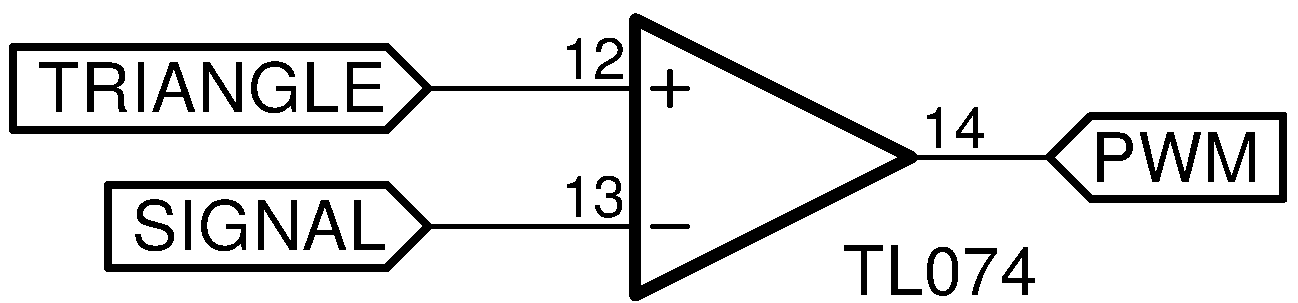
\includegraphics[width=6cm]{gfx/comp.pdf}
\caption{Komparator}
\label{fig:comp}
\end{floatingfigure}
\noindent
Der Komparator bildet das Kernstück zur Pulsweitenmodulation. Im wesentlichen vergleicht diese Komponente das im Dreiecksgenerator erzeugte Signal mit dem Eingangssignal und generiert damit die PWM (vgl. Abbildung \ref{fig:pwm}). Die Spezifikationen des für diese Aufgabe gewählten Operationsverstärkers sind von großer Bedeutung für die Funktionsfähigkeit und Skalierbarkeit des Gesamtsystems. Neben dem Stromverbrauch, der Betriebsspannung und der Slew-Rate ist auch die Beschaffbarkeit des Operationsvertärkers ein entscheidender Faktor. Für diese Anwendung wurde deswegen der TL074 gewählt, dieser zum einen durch die verwendete MOS-Technologie eine geringe Stromaufnahme von $< 14mA$ aufweist und zum Anderen mit einer Slew-Rate von $1V/ \mu s$ für diese Anwendung bestens geeignet ist.
\\

\subsection{Diodentreiber}
\label{sec:ksq}
\noindent
\begin{floatingfigure}[r]{6.5cm}
\centering
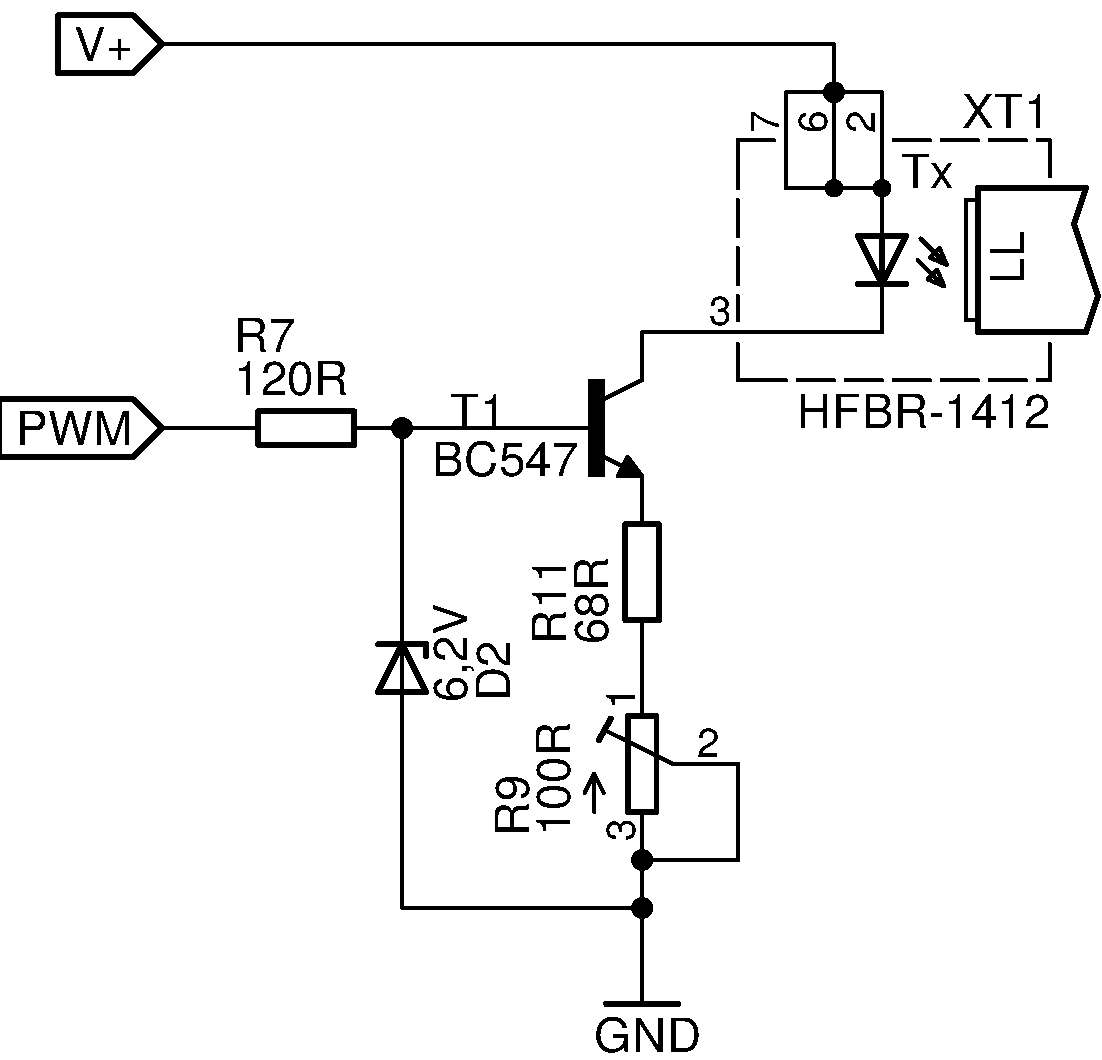
\includegraphics[width=6cm]{gfx/diodentreiber.pdf}
\caption{Diodentreiber}
\label{fig:diodedriver}
\end{floatingfigure}
Als Sendediode wird die Hoch\-leis\-tungs\-diode \textsc{HFBR-1412} verwendet. Diese benötigt minimal $30mA$ und maximal $120mA$. Da eine Diode ein Halbleiter ist, hat diese iene exponentielle Span\-nungs-Strom Kennlinie. Bei einer Versorgung mit konstanter Spannung kann durch thermische Rückkopplung der Strom, und damit die Verlustleistung, unkontrolliert ansteigen. Dies kann zur Zer\-störung des Bauteils führen. Aufgrund dessen wird der Diodentreiber als Kon\-stant\-strom\-quel\-le (KSQ) ausgeführt.

Die KSQ besteht aus $T_1$, $R_{11}$, $R_9$ und $D_2$. Der Widerstand $R_7$ dient lediglich der Begrenzung des Basisstromes von $T_1$ und der Strombegrenzung von $D_2$.
Die Zener-Diode $D_2$ hält die Spannung über der BE-Strecke von $T_1$ und den Widerständen $R_{11}$ und $R_9$ konstant. Da die Spannng über den Widerständen konstant ist, ist auch der Strom durch diese konstant. Daraus folgt, dass auch der Kollektorstrom von $T_1$ und somit auch der Strom durch die Leistungsdiode konstant ist.
Der Strom berechnet sich wie folgt.
\begin{align}
I_{konst} = \frac{U_z-U_{BE}}{R_9+R_{11}}
\end{align} 
Durch den Reihenwiderstand $R_{11}$	ist sichergestellt, dass auch bei Anschlag der Potentiometers zu $0\Omega$ der Strom nicht $130mA$ übersteigt. Der gesamte Einstellbereich für den Diodenstrom liegt bei $36mA < I_{konst}< 110mA$.
\newpage

\section{Schaltungsentwurf - Empfangseinheit}
Die Demodulation des Signals erfolgt im wesentlichen durch eine Tiefpass-Filterung. Das gesendete Signal muss allerdings erst vorbereitet werden. Dies geschieht durch eine Vorfilterung und anschließende Verstärkung. Ein Hochpass direkt am Ausgang der Empfangsdiode filtert DC-Anteile. Danach wird die Signalamplitude soweit verstärkt, dass der Signalverlauf wieder komplett rechteckig dem ursprüglichen PWM-Signal entsprechend verläuft. Dadurch wird die nachfolgende rekonstruierende Filterung durch den Butterworth-Tiefpass erst möglich. \\ Schlussendlich wird das zurückgewonnene Signal nach dem Rekonstruktionsfilter mit einer einstellbaren Endstufe final verstärkt, damit die Amplitude dem des gesendeten Signals entspricht.

%\begin{figure}[htbp]
%	\centering
%	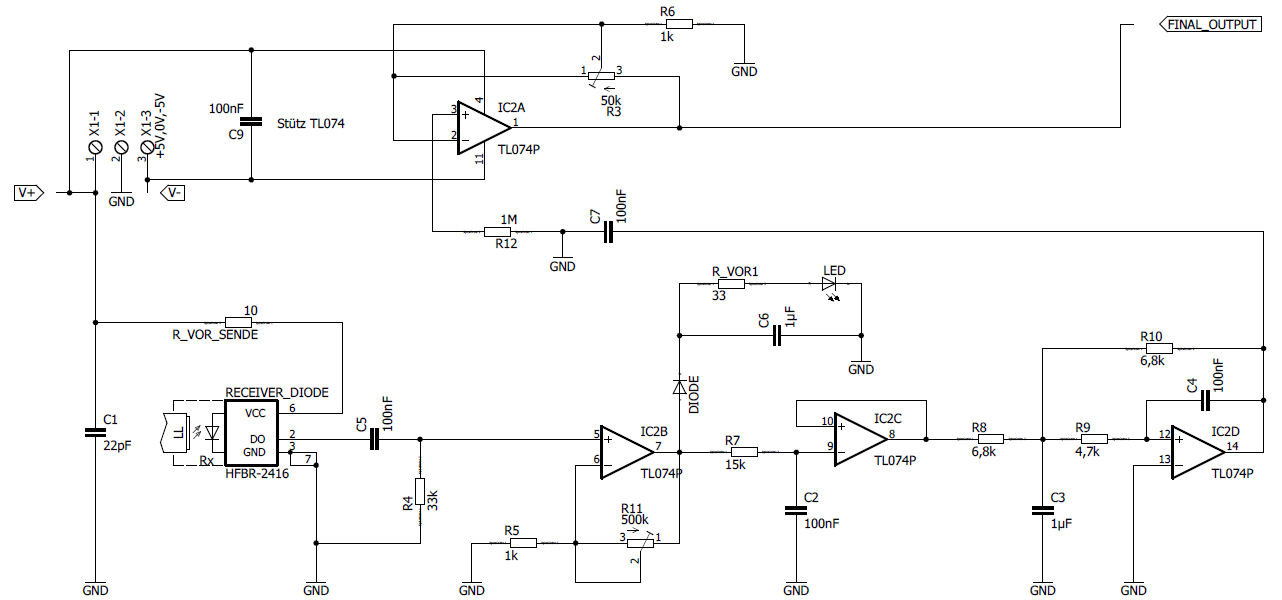
\includegraphics[angle=90, scale=0.36]{gfx/schaltung.png}
%	\caption{Empfängerschaltung (volles Querformat im Anhang)}
%\end{figure}
\subsection{Beschaltung der Empfangsdiode}
\label{subsec:receiver_schematic}
Für die Empfangsdiode \textsc{AVAGO HFBR-2416} ist folgendes Prinzipschaltbild aus dem Datenblatt\footnote{Avago, HFBR-2416, Seite 23, Figure 12 http://docs.avagotech.com/docs/AV02-0176EN} gegeben:
\begin{figure}[H]
	\centering
	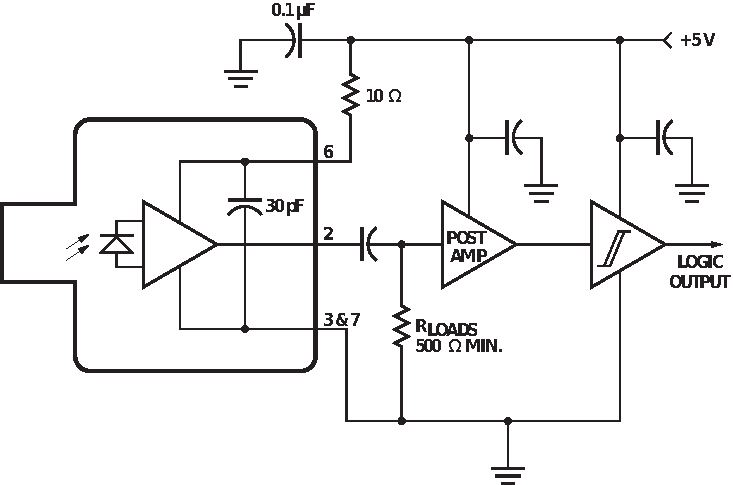
\includegraphics[scale=0.65]{gfx/hfbr.pdf}
	\caption{Prinzipschaltbild Empfangsdiode}
	\label{fig:basic_schematic} 
\end{figure}
\newpage
Die Prinzipschaltung wurde übernommen, um den Betrieb innerhalb der Spezifikationen zu gewährleisten. Die Bauteile sind so dimensioniert, dass die Grenzfrequenz des Hochpasses aus $R_4$ und $C_5$ unter dem Nachrichtensignal bei $50Hz$ liegt. Der Hochpass dient der Filterung von DC-Offsets seitens der Diode. \\
Für $R_4$ wurde $33k\Omega$ gewählt. Damit ergibt sich eine neue Grenzfrequenz von $ f_{g}=48,23Hz $.
Berechnung des Hochpasses: \\ 
Mit $C_5 = 100nF$ und $f_g=50Hz$  folgt:
\savebox\strutbox{$\vphantom{\dfrac11}$}
\begin{align}
		R &= \frac{1}{2 \pi \cdot f_g \cdot C}\\
		R &= \frac{1}{2 \pi \cdot 50 Hz \cdot 100nF}\\
		  &= 31,83k\Omega		 	
\end{align} 
\noindent


Nachfolgend die realisierte Schaltung:
\begin{figure}[htbp]
\centering
 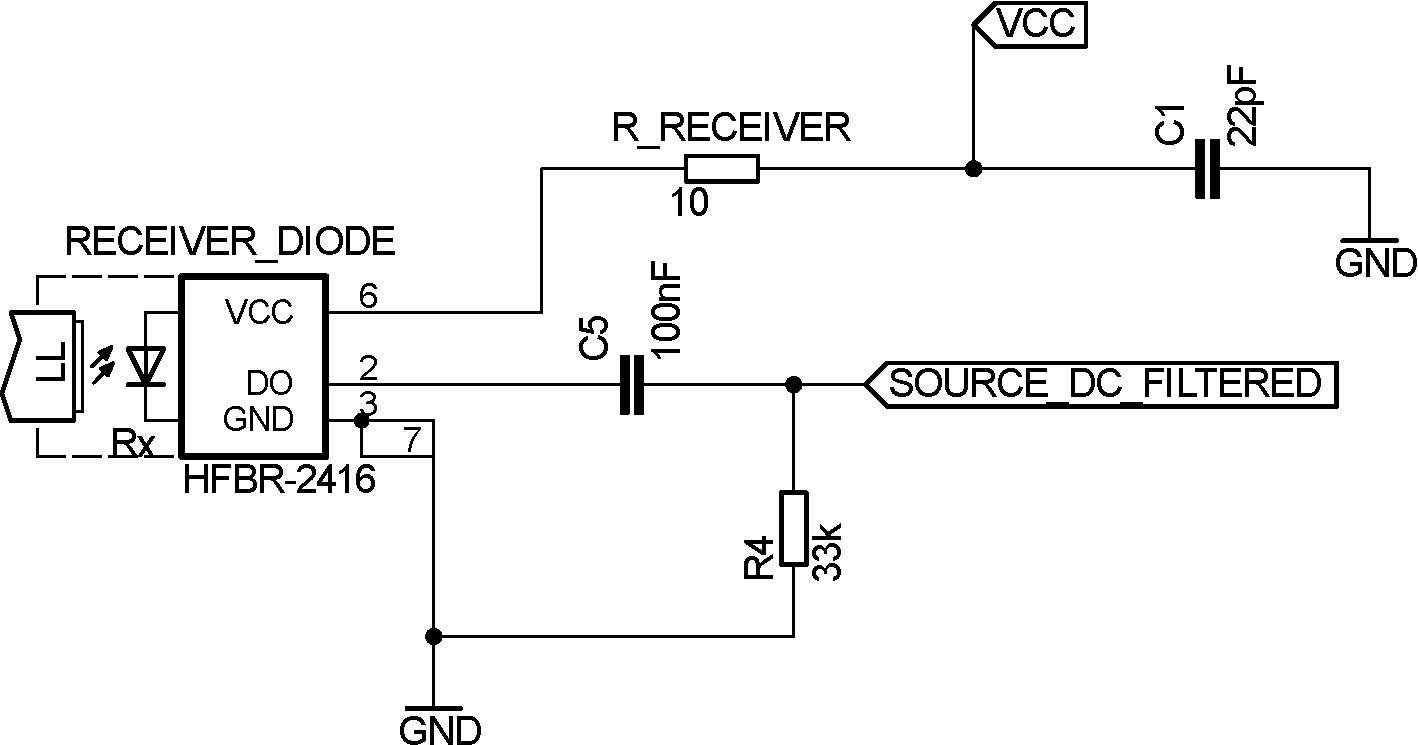
\includegraphics[scale=0.50]{gfx/receiver_part.pdf}
	\caption{Beschaltung Empfangsdiode}
\end{figure}
 
 

%\footnotetext{Quelle: Elektronik Vorlesungssunterlagen, Prof. Dr. Ralf Patz}
\newpage
\subsection{Signalaufbereitung}
\label{subsec:pre_amplifier}
Aufgrund der Leitungsdämpfung muss die Amplitude des modulierten Signals vor der Filterung durch den Rekonstruktionsfilter verstärkt werden (siehe Kapitel \ref{subsec:receiver_schematic} - Abbildung \ref{fig:basic_schematic}: \textsc{Postamp}).Das Signal wird über einen nicht-invertierenden Verstärker aufbereitet:
\begin{figure}[H]
\centering
 
\includegraphics[scale=0.40]{gfx/preamp}
	\caption{Vorverstärker}
\end{figure}
Damit die Schaltung für verschiedene Leitungslängen skalierbar ist, wurde eine variable Verstärkung bis zu einem Faktor von $V_u = 500$ gewählt. 
\begin{figure}[H]
\begin{minipage}{0.45\textwidth} 
	\begin{align}
	V_U&=1+\frac{R_4}{R_5}\\
	\frac{R_4}{R_5} &>> 1\\
	V_U&\approx\frac{R_4}{R_5} \label{eq1}
	\end{align}
	\end{minipage}
	\hfill
\begin{minipage}{0.45\textwidth}
		% \textwidth bezieht sich nun auf die Minipage
Für große Verstärkungen errechnet(siehe Formel\ref{eq1}\footnotemark) ist die 1 beim Nicht-Invertierenden Verstärker zu vernachlässligen. Die Verstärkung berechnet sich lediglich aus den beiden Widerständen $R_{5}$ und $R_{4}$. 
\end{minipage}
\end{figure}
\noindent
Mit $0\Omega < R_4 < 500k\Omega$ und $R_5=1k\Omega$ ist die Verstärkung von 0 bis 500 einstellbar.

\footnotetext{Quelle: Elektronik Vorlesungssunterlagen, Prof. Dr. Ralf Patz}
\begin{floatingfigure}[r]{7cm}
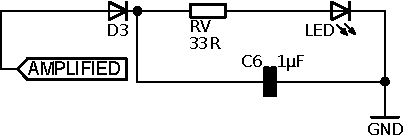
\includegraphics[width=6.5cm]{gfx/detect.pdf}
\caption{Signaldetektion}
\label{fig:detect}
\end{floatingfigure}
\noindent
Neben der Signalaufbereitung für die folgende Demodulation, wird das ver\-stär\-kte Signal auch für eine Signaldetektion aufbereitet. Zur Signalisierung wird eine Leuchtdiode an der Ge\-häu\-se\-front verwendet. Zur Glät\-tung der Spannung wird ein Kondensator parallel zu der Leuchtdiode mit Vorwiderstand geschaltet. Eine weitere Aufbereitung ist an dieser Stelle nicht notwendig, da das Trägersignal, als auch das Nachrichtensignal $\geq 50 Hz$  ist und somit für das menschliche Auge kein Flackern auftritt. 
\newpage
\subsection{Tiefpass}
Die Dimensionierung des Tiefpasses ist von zentraler Bedeutung bei der Rekonstruktion des Nachrichtensignals. Neben der Filtersteilheit und der Restwelligkeit sind Kennwerte wie Ausgangs- und Eingangswiderstand wichtig für die optmale Gestaltung des Tiefpasses.
\subsubsection{Filtercharakteristiken im Vergleich} 
\begin{floatingfigure}[r]{7cm}
	\includegraphics[width=6.5cm]{gfx/characteristics.png}
	\caption{Filtercharakteristiken}
\label{fig:characteristics}
\end{floatingfigure}
\noindent
Bei aktiven und mehrstufigen Filtertopologien gibt es eine große Auswahl an Fitlercharakteristiken, welche sich durch verschiedene Eigenschaften auszeichnen. Kennwerte für diese Charakteristiken sind Linearphasigkeit, Gruppenlaufzeit, sowie Restwelligkeit im Pass-und Sperrband. In Abbildung \ref{fig:characteristics} sind einige Charakteristiken beispielhaft dargestellt. Für die Rekonstruktion wird eine Butterworth-Charakteristik gewählt, da diese im Passband eine konstante Verstärkung aufweist, sowie keinen Peak kurz vor der Grenzfrequenz hat.\\

\subsubsection{Dimensionierung des Filters}
Zur Dimensionierung des Filters wurde die Designsoftware \textsc{FilterPro} von Texas Instruments verwendet. Als Designparameter wurden neben der Butter\-worth-Charakteristik, eine Verstärkung von 0dB, eine Dämpfung von 9dB je Dekade(Filter 3. Ordnung), Bauteile der E12 Reihe, eine Grenzfrequenz von $f_g=100Hz$ und eine Multiple-Feedback Topologie vorgegeben. Diese Topologie hat im Gegensatz zur Sallen-Key Topologie den Vorteil eines hohen Ausgangswiderstandes. Die Verstärkung von 0dB wird gewählt, da eine Endstufe mit variabler Verstärkung dieser Komponente folgt.
\begin{figure}[H]
	\centering
	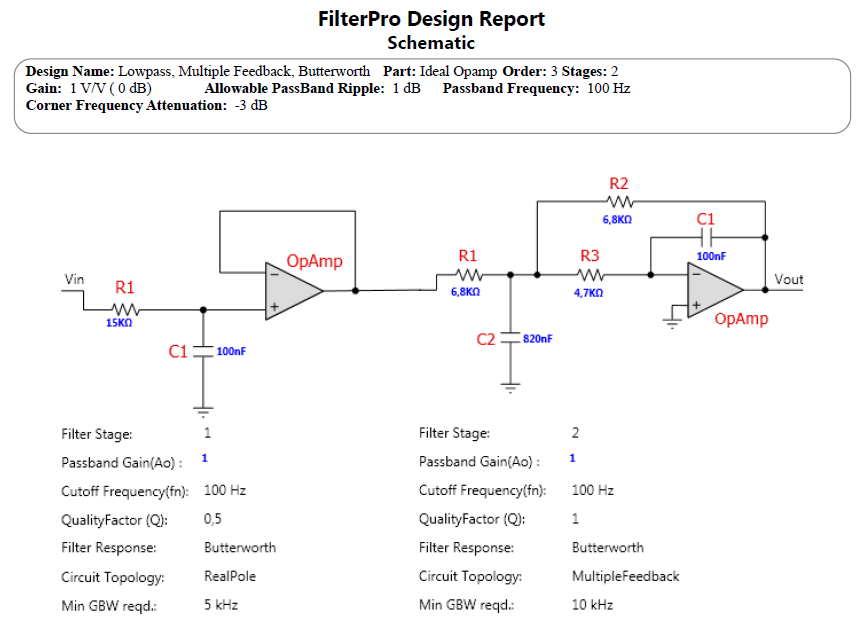
\includegraphics[scale=0.575]{gfx/Butterworth_FilterPro.png}
	\caption{Auszug Design Report}
	\label{fig:design_report}
\end{figure}
\noindent
Der Designreport zeigt die gewünschten Filterparameter. Besonders wichtig an dieser Stelle ist die benötigte Unity-Gain(Gain-Bandwidth-Product), welche sich mit maximal $10kHz$ innerhalb der Spezifikationen vom \textsc{TL074} befinden. Darüber hinaus wurde aufgrund besserer Beschaffbarkeit $C_2$ zu $1\mu F$ gewählt.
\begin{figure}[H]
	\centering
	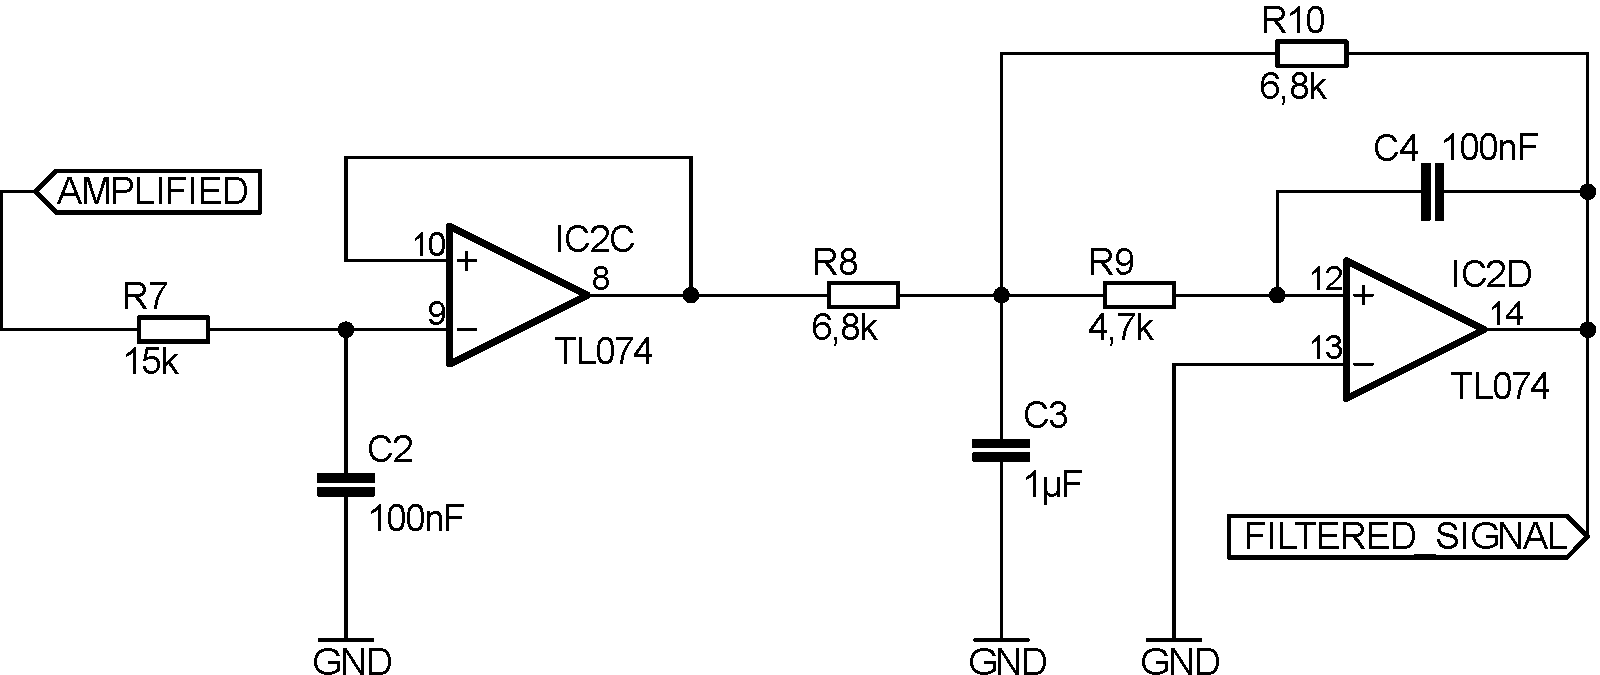
\includegraphics[scale=0.5]{gfx/filter.pdf}
	\caption{Butterworth-Tiefpass}
\end{figure}
\noindent
Der Widerstand $R_7$ und der Kondensator $C_2$ bilden als passiver Tiefpass die erste Filterstufe. Diese ist mit dem linken Operationsverstärker, welcher als Spannungsfolger beschaltet ist von der nachfolgenden zweiten Filterstufe entkoppelt. Mit $R_8$ und $C_3$ folgt ein weiterer passiver Tiefpass. Der letzte Teil des Filters ist ein aktiver Tiefpass, der sich aus dem zweiten Operationsverstärker und den Widerständen $R_9$ ,$R_{10}$, sowie dem Kondensator $C_4$ zusammensetzt.








\subsection{Endstufe}
Der letzte Teil der Empfangseinheit besteht aus einem weiteren Verstärker und einem vorgeschalteten Hochpass. Der Hochpass hat eine Grenzfrequenz von $f_{g} \approx 1,59Hz$ und dient der Filterung vorangegangener DC-Offsets. Wie in Kapitel \ref{subsec:pre_amplifier} bereits gezeigt, ist die Verstärkung ausschließlich von den beiden Widerständen abhänging. Die Verstärkung des Verstärkers ist somit über das Potentiometer von 0 bis 50 einstellbar.
\begin{figure}[H]
	\centering
	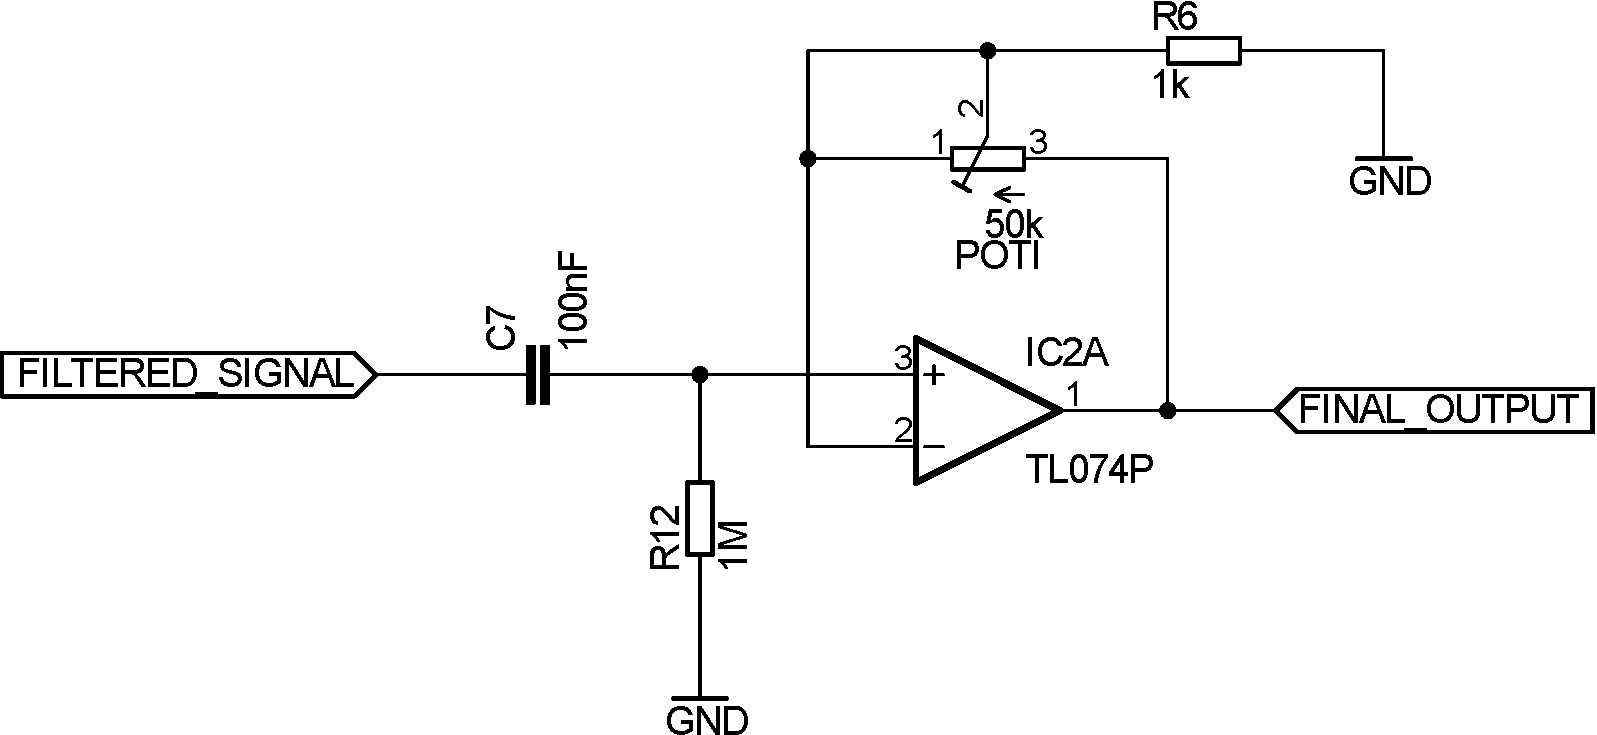
\includegraphics[scale=0.5]{gfx/post_amplifier.pdf}
	\caption{Endstufe}
\end{figure}

\section{Simulation kritischer Schaltungsteile}
\subsection{Sendeeinheit}
\subsubsection{Eingangsteil}
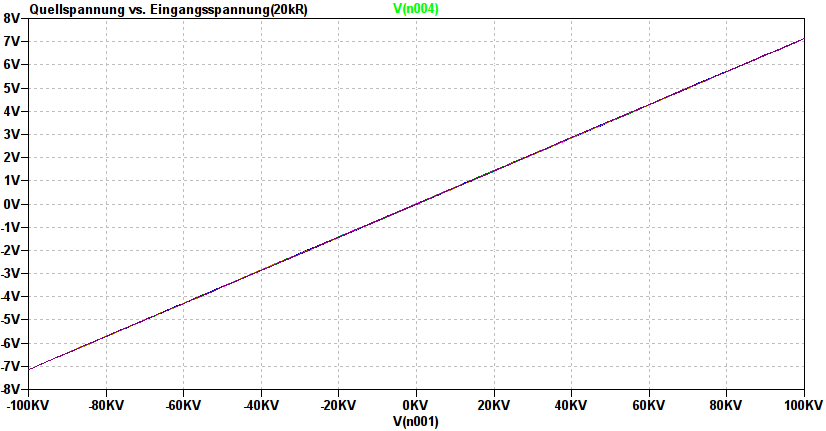
\includegraphics[scale=0.5]{gfx/simTx/Impedance20k.png}
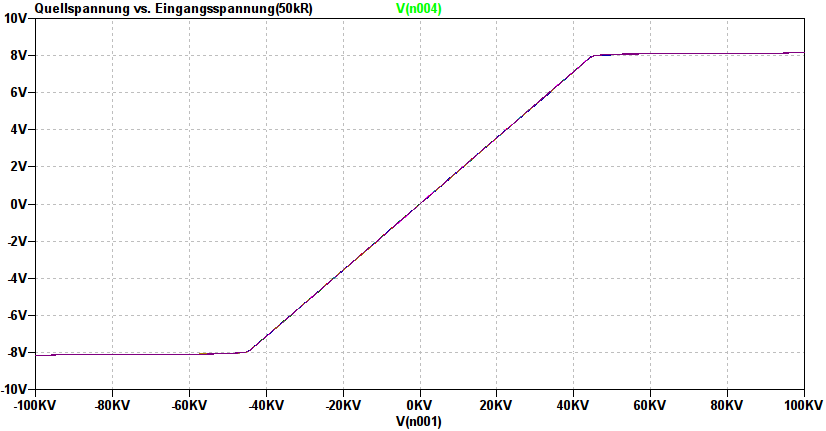
\includegraphics[scale=0.5]{gfx/simTx/Impedance50k.png}

\subsubsection{Millerintegrator}
\begin{float}
\centering
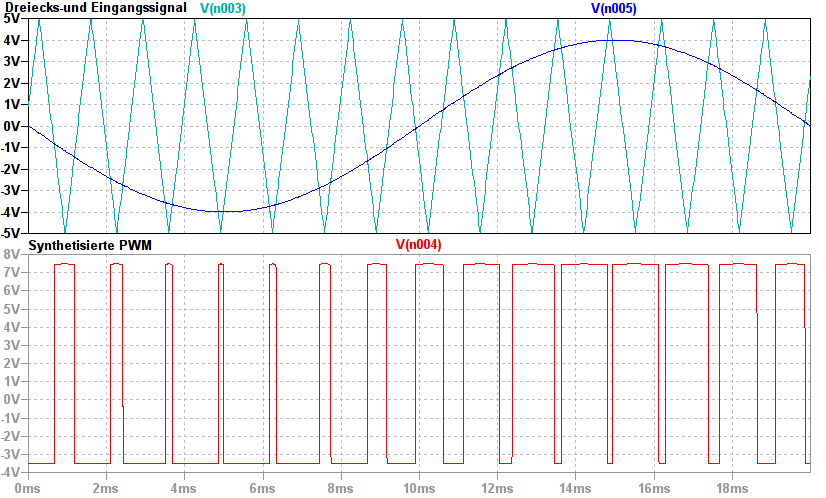
\includegraphics[scale=0.5]{gfx/simTx/PWMsynth.png}
\end{float}
\subsubsection{Diodentreiber}
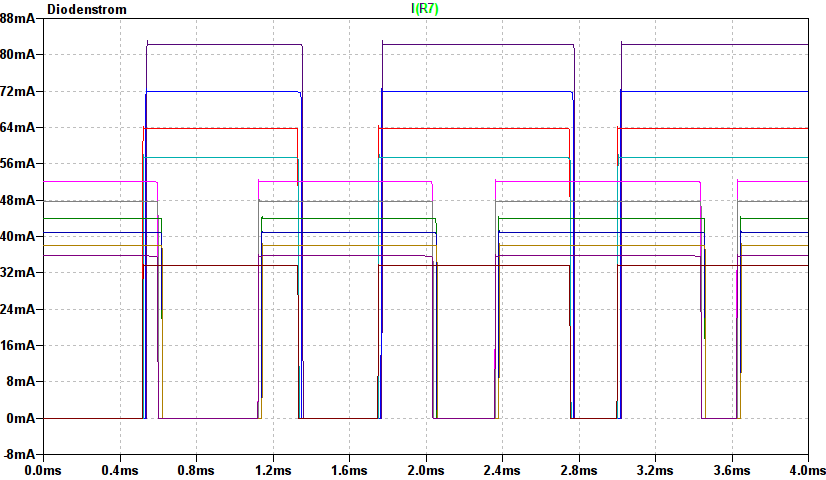
\includegraphics[scale=0.5]{gfx/simTx/DiodeCurrent.png}
\subsection{Empfangseinheit}
\includegraphics[scale=1]{gfx/simRx/characteristics.png}
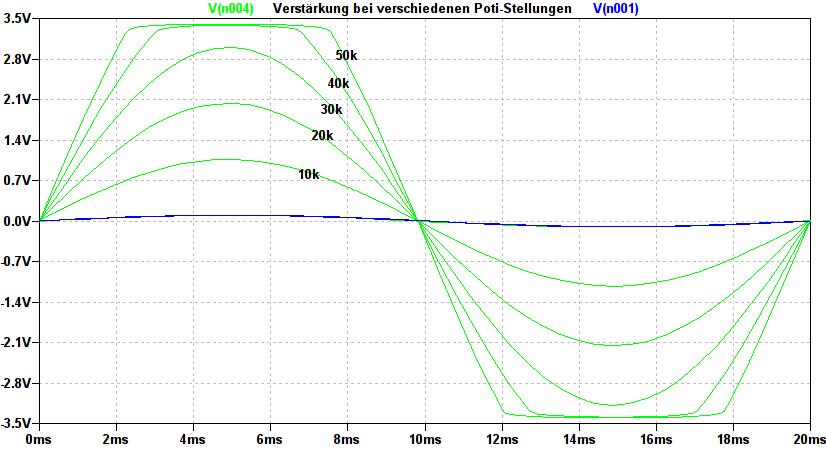
\includegraphics[scale=0.5]{gfx/simRx/amplification.png}
\subsection{Empfangseinheit}
\subsubsection{Tiefpass}
Die folgende Simulation(Abb. \ref{fig:frequencyResponse}) zeigt die Simulation des Butterworth-Tiefpasses durch FilterPro. Es sind der Frequenzgang(obere Kurve) und der Phasengang(untere Kurve) zu sehen. Der Tiefpass hat ab 100 Hz eine konstante Dämpfung von 60 dB je Dekade und zeigt damit das Verhalten eines Tiefpasses dritter Ordnung. Das zu übertragende Signal(50 Hz  Sinus) wird nicht gedämpft(0dB) und hat eine Phasenverschiebung von ca. $105^o$.
\begin{figure}[H]
\centering
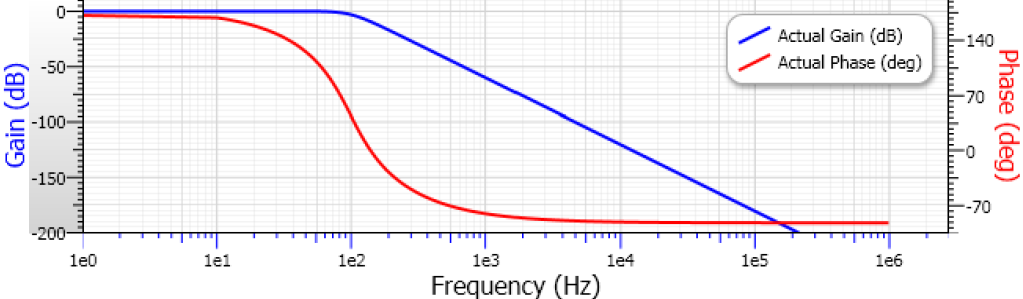
\includegraphics[scale=0.35]{gfx/simRx/FilterPro.png}
\caption{Simulation Frequenz-und Phasengang Butterworth-Tiefpass}
	\label{fig:frequencyResponse} 
\end{figure}


\subsubsection{Ausgangsverstärker}
Abbildung \ref{fig:amplifier} zeigt die Simulation der Verstärkung des Ausgangsverstärkers(Abschnitt \ref{sec:endamp}). Zur Simulation wurde ein Sinussignal von 100mV Amplitude und einer Frequenz von 50Hz eingeprägt. Das Potentiometer $"POTI"$(Abb. \ref{fig:endamp}) wurde mittels parametrischer Simulartion von $0 - 50k\Omega$ varriert und somit verschiedene Verstärkungsfaktoren von 0 bis 50 simuliert. Es ist zu erkennen, dass bei erreichen der Betriebsspannung der Verstärker clippt. 
\begin{figure}[H]
\centering
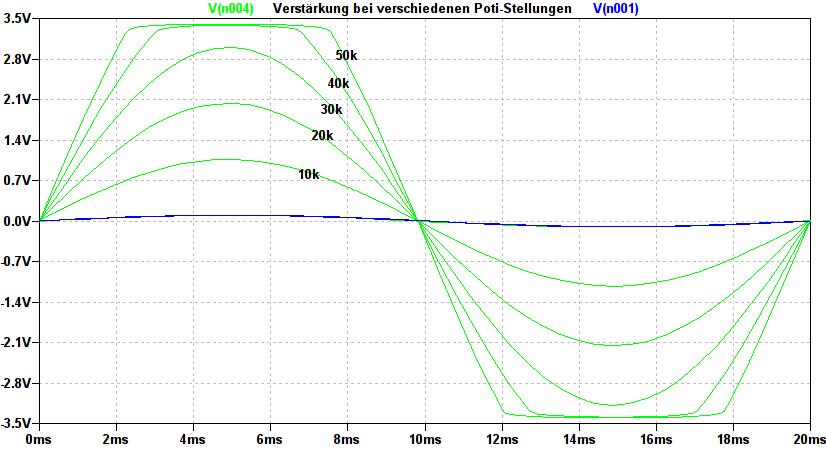
\includegraphics[scale=0.5]{gfx/simRx/amplification.png}
\caption{Simulation Ausgangsverstärker}
	\label{fig:amplifier} 
\end{figure}


\section{Messungen}

\subsection{Sendeeinheit}
Die folgenden Grafiken(Abb. \ref{fig:measMiller}) zeigen das Eingangssignal(obere Kurve), das Dreieckssignal des Miller-Integrator(mittlere Kurve) und die daraus synthetisierte PWM(untere Kurve) in jeweils 2 Zeitauflösungen. Die obere Grafik ist dabei mit 2 ms/DIV und die untere Grafik mit 1ms/DIV aufgelöst. Diese Messung bestätigt damit die Simluation aus Abschnitt \ref{sec:simMiller}. Die Frequenz des wurde zu Demonstrationszwecken auf ca. 2kHz verringert um die Änderung des Tastverhältnisses des Rechtecksignals reltiv zum Eingangssignal darzustellen. Gut zu erkennen ist, dass sich die Fläche unter dem Rechtecksignal relativ zum Eingangssignal ändert und damit der Effektivwert des Rechtecksignals.(siehe Abschnitt \ref{sec:pwmTheory}).
\begin{figure}[H]
	\centering
	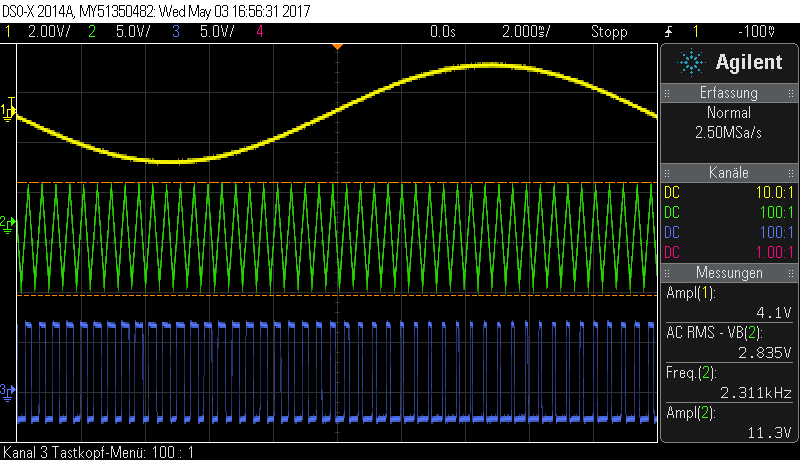
\includegraphics[scale=0.45]{gfx/osziScreens/scope_3.png}
	\caption{Eingangssignal,Dreieck und PWM grob aufgelöst}
	\label{fig:measMiller}
\end{figure}

\begin{figure}[H]
	\centering
	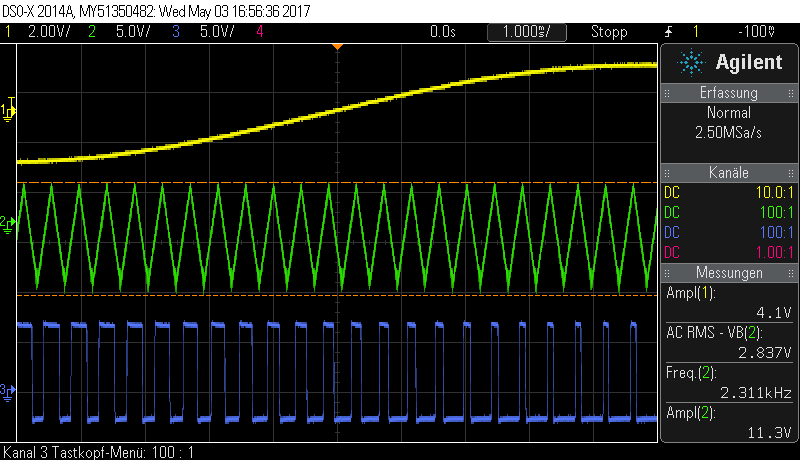
\includegraphics[scale=0.45]{gfx/osziScreens/scope_4.png}
	\caption{Eingangssignal,Dreieck und PWM genauer aufgelöst}
	\label{fig:measMiller}
\end{figure}
\subsection{Empfangseinheit}
Die folgenden Messungen zeigen die Filterung des Empfangssignals in verschiedenen Filterstufen(Kurven je Grafik) und zu verschiedenen Zeitauflösung\-en(obere und untere Grafik). Die obere Kurve zeigt das empfangene Signal direkt vor dem Tiefpass. Die mittlere Kurve zeigt das Signal nach dem passiven Tiefpass(vgl. Abb. \ref{fig:design_report} $R_1,C_1$). Die untere Kurve zeigt das empfangene Signal nach dem Tiefpass und vor dem Endverstärker. Die Grafiken zeigen die Kurven jeweils bei einer Zeitauflösung von 10ms/DIV(obere Grafik) und 2ms/DIV(untere Grafik. Bei der Zeitauflösung von 2ms/DIV ist sehr gut zu erkennen, dass nach dem ersten Tiefpass, das Signal aus einem Sinus, welcher mit einem Dreieckssignal überlagert ist, besteht und nach weiterer Filterung dieses hochfrequente Dreieckssignal komplett verschwindet. Dies bestätigt den Frequenzgang aus Abbildung \ref{fig:frequencyResponse}.
\begin{figure}[H]
	\centering
	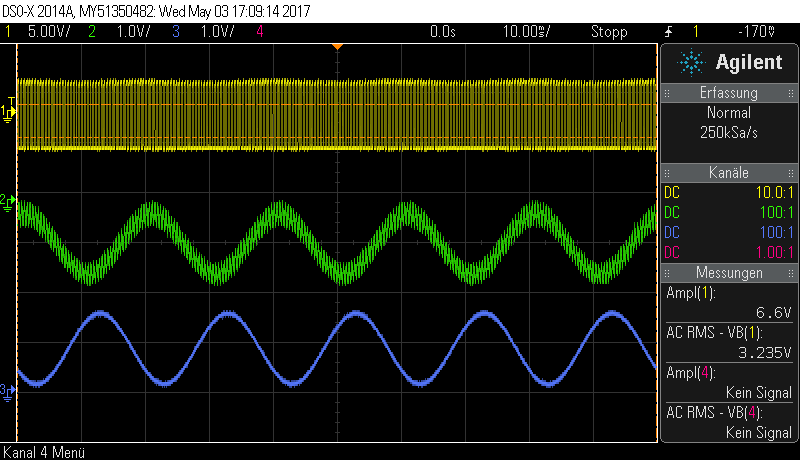
\includegraphics[scale=0.45]{gfx/osziScreens/scope_10.png}
	\caption{Emfangssignal in verschiedenen Filterstufen grob aufgelöst}
\end{figure}

\begin{figure}[H]
	\centering
	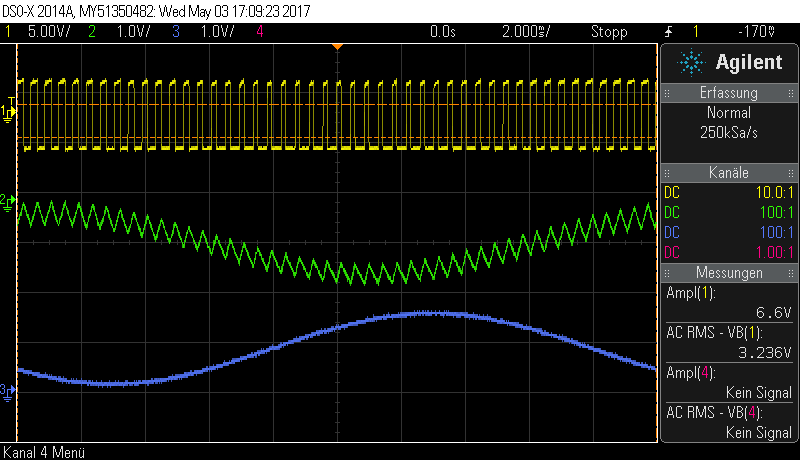
\includegraphics[scale=0.45]{gfx/osziScreens/scope_11.png}
	\caption{Emfangssignal in verschiedenen Filterstufen genauer aufgelöst}
\end{figure}
\subsection{Gesamtsystem}
In dieser Messung wurde die Linearität des Gesamtsystems geprüft. Die obere Kurve zeigt das Eingangssignal vor der Sendeeinheit, die untere Kurve zeigt das Ausgangssignal nach der Empfangseinheit. Zu Testzwecken wurde die Verstärkung der Empfangseinheit, so justiert, dass bei kleiner Eingangsspannung(ca. $4V_{pp}$) an der Sendeeinheit auch selbige von der Empfangseinheit am Ausgang wiedergegeben wird. 
\begin{figure}[H]
  \centering
   \subfigure[5V Eingangsspannung]{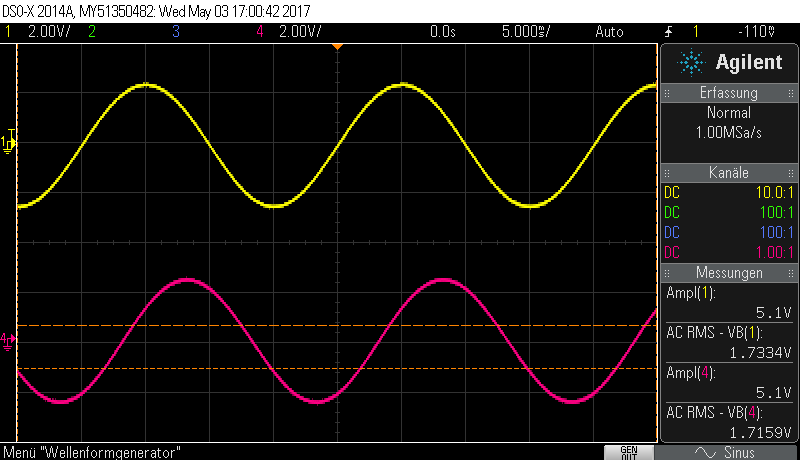
\includegraphics[scale=0.2]{gfx/osziScreens/scope_6.png}}\qquad
   \subfigure[4V Eingangsspannung]{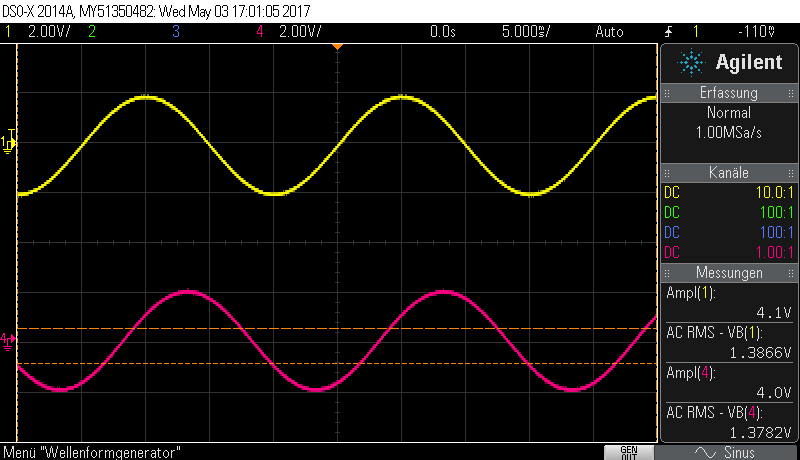
\includegraphics[scale=0.2]{gfx/osziScreens/scope_7.png}}\\
   \subfigure[3V Eingangsspannung]{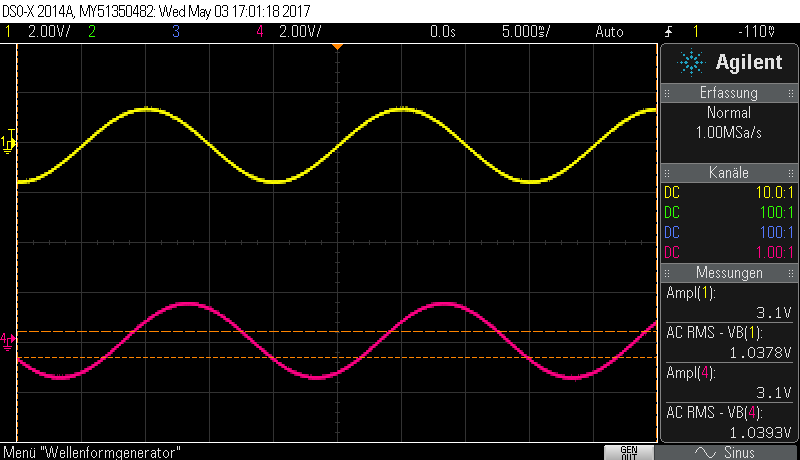
\includegraphics[scale=0.2]{gfx/osziScreens/scope_8.png}}\qquad
   \subfigure[2V Eingangsspannung]{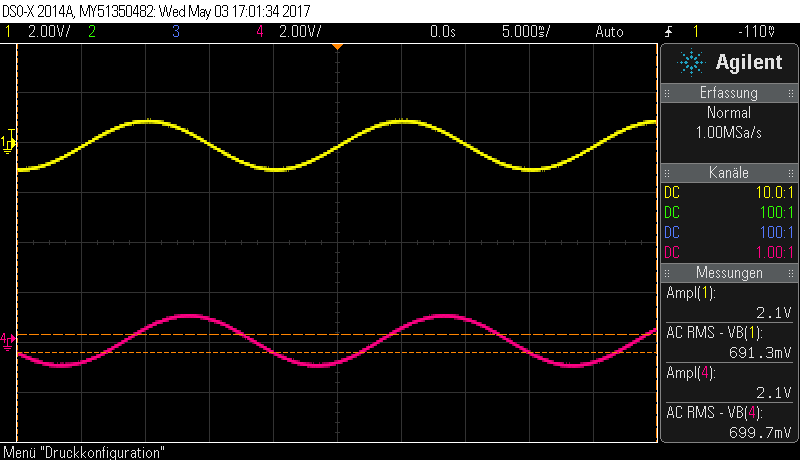
\includegraphics[scale=0.2]{gfx/osziScreens/scope_9.png}}
  \caption{Linearität des Gesamtsystems}
\end{figure}

Zur Überprüfung der Linearität wird der Quotient aus Eingangssignal und Ausgangssignal gebildet. Die folgende Tabelle(Tabelle \ref{tab:lin}) zeigt einen annährend gleichbleibenden Quotienten und somit, dass das Gesamtsystem linear ist. 
\begin{table}[H]
\centering
\begin{tabular}{clll}
\cline{1-4}
Messung & $\frac{U_{ein}}{V}$ & $\frac{U_{aus}}{V}$ &$\frac{U_{ein}}{U_{aus}}$ \\ 
\cline{1-4}
a & 5,1                                        & 5,1                                       & 1                         \\
b & 4,1                                        & 4,0                                       & 1.025                     \\
c & 3,1                                        & 3,1                                       & 1                         \\
d & 2,1                                        & 2,1                                       & 1                        
\end{tabular}
\caption{Linearitätsprüfung des Gesamtsystems}
\label{tab:lin} 
\end{table}







\section{Justierung der Übertragungsstrecke}
\subsection{Rahmenbedingungen}
Zur Justierung der Übertragungsstrecke sind folgende Rahmenbedingungen zu beachten:
\begin{itemize}
\item maximale Eingangsspannung der Sendeeinheit(7V)
\item maximale Ausgangsspannung der Empfangseinheit(5V)
\item Linearität der Modulation
\item Einfacher Umrechnungsfaktor für das gegebene System
\end{itemize}

\subsection{Berechnung des Innenwiderstandes}
Es besteht die Möglichkleit die Impedanz der Sendeeinheit mittels Kippschalter umzuschalten. In der ersten Schalterstellung kann eine Impedanz von 0 bis $10k\Omega$ vorgegeben werden, in der zweiten eine Impedanz von 0 bis $50k\Omega$. Diese werden mittels Trimmpotentiometers eingestellt. 
\subsection{Messergebnisse}
Wie in Abb. \ref{fig:9k89} zu sehen ist, verhält sich der Aufbau über den gesamten 100kV Messbereich linear. Die Funktion der dargestellten Regressionsgeraden lautet:
\begin{equation}
y_i = 50,387569655 \cdot x_i - 0,97547594819
\label{math:regress100kV}
\end{equation} 
  	\begin{figure}[H]
		%% Creator: Matplotlib, PGF backend
%%
%% To include the figure in your LaTeX document, write
%%   \input{<filename>.pgf}
%%
%% Make sure the required packages are loaded in your preamble
%%   \usepackage{pgf}
%%
%% Figures using additional raster images can only be included by \input if
%% they are in the same directory as the main LaTeX file. For loading figures
%% from other directories you can use the `import` package
%%   \usepackage{import}
%% and then include the figures with
%%   \import{<path to file>}{<filename>.pgf}
%%
%% Matplotlib used the following preamble
%%   \usepackage{fontspec}
%%   \setmainfont{DejaVu Serif}
%%   \setsansfont{DejaVu Sans}
%%   \setmonofont{DejaVu Sans Mono}
%%
\begingroup%
\makeatletter%
\begin{pgfpicture}%
\pgfpathrectangle{\pgfpointorigin}{\pgfqpoint{6.000000in}{4.000000in}}%
\pgfusepath{use as bounding box, clip}%
\begin{pgfscope}%
\pgfsetbuttcap%
\pgfsetmiterjoin%
\definecolor{currentfill}{rgb}{1.000000,1.000000,1.000000}%
\pgfsetfillcolor{currentfill}%
\pgfsetlinewidth{0.000000pt}%
\definecolor{currentstroke}{rgb}{1.000000,1.000000,1.000000}%
\pgfsetstrokecolor{currentstroke}%
\pgfsetdash{}{0pt}%
\pgfpathmoveto{\pgfqpoint{0.000000in}{0.000000in}}%
\pgfpathlineto{\pgfqpoint{6.000000in}{0.000000in}}%
\pgfpathlineto{\pgfqpoint{6.000000in}{4.000000in}}%
\pgfpathlineto{\pgfqpoint{0.000000in}{4.000000in}}%
\pgfpathclose%
\pgfusepath{fill}%
\end{pgfscope}%
\begin{pgfscope}%
\pgfsetbuttcap%
\pgfsetmiterjoin%
\definecolor{currentfill}{rgb}{1.000000,1.000000,1.000000}%
\pgfsetfillcolor{currentfill}%
\pgfsetlinewidth{0.000000pt}%
\definecolor{currentstroke}{rgb}{0.000000,0.000000,0.000000}%
\pgfsetstrokecolor{currentstroke}%
\pgfsetstrokeopacity{0.000000}%
\pgfsetdash{}{0pt}%
\pgfpathmoveto{\pgfqpoint{0.750000in}{0.500000in}}%
\pgfpathlineto{\pgfqpoint{5.400000in}{0.500000in}}%
\pgfpathlineto{\pgfqpoint{5.400000in}{3.520000in}}%
\pgfpathlineto{\pgfqpoint{0.750000in}{3.520000in}}%
\pgfpathclose%
\pgfusepath{fill}%
\end{pgfscope}%
\begin{pgfscope}%
\pgfsetbuttcap%
\pgfsetroundjoin%
\definecolor{currentfill}{rgb}{0.000000,0.000000,0.000000}%
\pgfsetfillcolor{currentfill}%
\pgfsetlinewidth{0.803000pt}%
\definecolor{currentstroke}{rgb}{0.000000,0.000000,0.000000}%
\pgfsetstrokecolor{currentstroke}%
\pgfsetdash{}{0pt}%
\pgfsys@defobject{currentmarker}{\pgfqpoint{0.000000in}{-0.048611in}}{\pgfqpoint{0.000000in}{0.000000in}}{%
\pgfpathmoveto{\pgfqpoint{0.000000in}{0.000000in}}%
\pgfpathlineto{\pgfqpoint{0.000000in}{-0.048611in}}%
\pgfusepath{stroke,fill}%
}%
\begin{pgfscope}%
\pgfsys@transformshift{1.258367in}{0.500000in}%
\pgfsys@useobject{currentmarker}{}%
\end{pgfscope}%
\end{pgfscope}%
\begin{pgfscope}%
\pgftext[x=1.258367in,y=0.402778in,,top]{\sffamily\fontsize{10.000000}{12.000000}\selectfont 0.25}%
\end{pgfscope}%
\begin{pgfscope}%
\pgfsetbuttcap%
\pgfsetroundjoin%
\definecolor{currentfill}{rgb}{0.000000,0.000000,0.000000}%
\pgfsetfillcolor{currentfill}%
\pgfsetlinewidth{0.803000pt}%
\definecolor{currentstroke}{rgb}{0.000000,0.000000,0.000000}%
\pgfsetstrokecolor{currentstroke}%
\pgfsetdash{}{0pt}%
\pgfsys@defobject{currentmarker}{\pgfqpoint{0.000000in}{-0.048611in}}{\pgfqpoint{0.000000in}{0.000000in}}{%
\pgfpathmoveto{\pgfqpoint{0.000000in}{0.000000in}}%
\pgfpathlineto{\pgfqpoint{0.000000in}{-0.048611in}}%
\pgfusepath{stroke,fill}%
}%
\begin{pgfscope}%
\pgfsys@transformshift{1.816644in}{0.500000in}%
\pgfsys@useobject{currentmarker}{}%
\end{pgfscope}%
\end{pgfscope}%
\begin{pgfscope}%
\pgftext[x=1.816644in,y=0.402778in,,top]{\sffamily\fontsize{10.000000}{12.000000}\selectfont 0.50}%
\end{pgfscope}%
\begin{pgfscope}%
\pgfsetbuttcap%
\pgfsetroundjoin%
\definecolor{currentfill}{rgb}{0.000000,0.000000,0.000000}%
\pgfsetfillcolor{currentfill}%
\pgfsetlinewidth{0.803000pt}%
\definecolor{currentstroke}{rgb}{0.000000,0.000000,0.000000}%
\pgfsetstrokecolor{currentstroke}%
\pgfsetdash{}{0pt}%
\pgfsys@defobject{currentmarker}{\pgfqpoint{0.000000in}{-0.048611in}}{\pgfqpoint{0.000000in}{0.000000in}}{%
\pgfpathmoveto{\pgfqpoint{0.000000in}{0.000000in}}%
\pgfpathlineto{\pgfqpoint{0.000000in}{-0.048611in}}%
\pgfusepath{stroke,fill}%
}%
\begin{pgfscope}%
\pgfsys@transformshift{2.374921in}{0.500000in}%
\pgfsys@useobject{currentmarker}{}%
\end{pgfscope}%
\end{pgfscope}%
\begin{pgfscope}%
\pgftext[x=2.374921in,y=0.402778in,,top]{\sffamily\fontsize{10.000000}{12.000000}\selectfont 0.75}%
\end{pgfscope}%
\begin{pgfscope}%
\pgfsetbuttcap%
\pgfsetroundjoin%
\definecolor{currentfill}{rgb}{0.000000,0.000000,0.000000}%
\pgfsetfillcolor{currentfill}%
\pgfsetlinewidth{0.803000pt}%
\definecolor{currentstroke}{rgb}{0.000000,0.000000,0.000000}%
\pgfsetstrokecolor{currentstroke}%
\pgfsetdash{}{0pt}%
\pgfsys@defobject{currentmarker}{\pgfqpoint{0.000000in}{-0.048611in}}{\pgfqpoint{0.000000in}{0.000000in}}{%
\pgfpathmoveto{\pgfqpoint{0.000000in}{0.000000in}}%
\pgfpathlineto{\pgfqpoint{0.000000in}{-0.048611in}}%
\pgfusepath{stroke,fill}%
}%
\begin{pgfscope}%
\pgfsys@transformshift{2.933198in}{0.500000in}%
\pgfsys@useobject{currentmarker}{}%
\end{pgfscope}%
\end{pgfscope}%
\begin{pgfscope}%
\pgftext[x=2.933198in,y=0.402778in,,top]{\sffamily\fontsize{10.000000}{12.000000}\selectfont 1.00}%
\end{pgfscope}%
\begin{pgfscope}%
\pgfsetbuttcap%
\pgfsetroundjoin%
\definecolor{currentfill}{rgb}{0.000000,0.000000,0.000000}%
\pgfsetfillcolor{currentfill}%
\pgfsetlinewidth{0.803000pt}%
\definecolor{currentstroke}{rgb}{0.000000,0.000000,0.000000}%
\pgfsetstrokecolor{currentstroke}%
\pgfsetdash{}{0pt}%
\pgfsys@defobject{currentmarker}{\pgfqpoint{0.000000in}{-0.048611in}}{\pgfqpoint{0.000000in}{0.000000in}}{%
\pgfpathmoveto{\pgfqpoint{0.000000in}{0.000000in}}%
\pgfpathlineto{\pgfqpoint{0.000000in}{-0.048611in}}%
\pgfusepath{stroke,fill}%
}%
\begin{pgfscope}%
\pgfsys@transformshift{3.491475in}{0.500000in}%
\pgfsys@useobject{currentmarker}{}%
\end{pgfscope}%
\end{pgfscope}%
\begin{pgfscope}%
\pgftext[x=3.491475in,y=0.402778in,,top]{\sffamily\fontsize{10.000000}{12.000000}\selectfont 1.25}%
\end{pgfscope}%
\begin{pgfscope}%
\pgfsetbuttcap%
\pgfsetroundjoin%
\definecolor{currentfill}{rgb}{0.000000,0.000000,0.000000}%
\pgfsetfillcolor{currentfill}%
\pgfsetlinewidth{0.803000pt}%
\definecolor{currentstroke}{rgb}{0.000000,0.000000,0.000000}%
\pgfsetstrokecolor{currentstroke}%
\pgfsetdash{}{0pt}%
\pgfsys@defobject{currentmarker}{\pgfqpoint{0.000000in}{-0.048611in}}{\pgfqpoint{0.000000in}{0.000000in}}{%
\pgfpathmoveto{\pgfqpoint{0.000000in}{0.000000in}}%
\pgfpathlineto{\pgfqpoint{0.000000in}{-0.048611in}}%
\pgfusepath{stroke,fill}%
}%
\begin{pgfscope}%
\pgfsys@transformshift{4.049751in}{0.500000in}%
\pgfsys@useobject{currentmarker}{}%
\end{pgfscope}%
\end{pgfscope}%
\begin{pgfscope}%
\pgftext[x=4.049751in,y=0.402778in,,top]{\sffamily\fontsize{10.000000}{12.000000}\selectfont 1.50}%
\end{pgfscope}%
\begin{pgfscope}%
\pgfsetbuttcap%
\pgfsetroundjoin%
\definecolor{currentfill}{rgb}{0.000000,0.000000,0.000000}%
\pgfsetfillcolor{currentfill}%
\pgfsetlinewidth{0.803000pt}%
\definecolor{currentstroke}{rgb}{0.000000,0.000000,0.000000}%
\pgfsetstrokecolor{currentstroke}%
\pgfsetdash{}{0pt}%
\pgfsys@defobject{currentmarker}{\pgfqpoint{0.000000in}{-0.048611in}}{\pgfqpoint{0.000000in}{0.000000in}}{%
\pgfpathmoveto{\pgfqpoint{0.000000in}{0.000000in}}%
\pgfpathlineto{\pgfqpoint{0.000000in}{-0.048611in}}%
\pgfusepath{stroke,fill}%
}%
\begin{pgfscope}%
\pgfsys@transformshift{4.608028in}{0.500000in}%
\pgfsys@useobject{currentmarker}{}%
\end{pgfscope}%
\end{pgfscope}%
\begin{pgfscope}%
\pgftext[x=4.608028in,y=0.402778in,,top]{\sffamily\fontsize{10.000000}{12.000000}\selectfont 1.75}%
\end{pgfscope}%
\begin{pgfscope}%
\pgfsetbuttcap%
\pgfsetroundjoin%
\definecolor{currentfill}{rgb}{0.000000,0.000000,0.000000}%
\pgfsetfillcolor{currentfill}%
\pgfsetlinewidth{0.803000pt}%
\definecolor{currentstroke}{rgb}{0.000000,0.000000,0.000000}%
\pgfsetstrokecolor{currentstroke}%
\pgfsetdash{}{0pt}%
\pgfsys@defobject{currentmarker}{\pgfqpoint{0.000000in}{-0.048611in}}{\pgfqpoint{0.000000in}{0.000000in}}{%
\pgfpathmoveto{\pgfqpoint{0.000000in}{0.000000in}}%
\pgfpathlineto{\pgfqpoint{0.000000in}{-0.048611in}}%
\pgfusepath{stroke,fill}%
}%
\begin{pgfscope}%
\pgfsys@transformshift{5.166305in}{0.500000in}%
\pgfsys@useobject{currentmarker}{}%
\end{pgfscope}%
\end{pgfscope}%
\begin{pgfscope}%
\pgftext[x=5.166305in,y=0.402778in,,top]{\sffamily\fontsize{10.000000}{12.000000}\selectfont 2.00}%
\end{pgfscope}%
\begin{pgfscope}%
\pgftext[x=3.075000in,y=0.212809in,,top]{\sffamily\fontsize{10.000000}{12.000000}\selectfont U1/V}%
\end{pgfscope}%
\begin{pgfscope}%
\pgfsetbuttcap%
\pgfsetroundjoin%
\definecolor{currentfill}{rgb}{0.000000,0.000000,0.000000}%
\pgfsetfillcolor{currentfill}%
\pgfsetlinewidth{0.803000pt}%
\definecolor{currentstroke}{rgb}{0.000000,0.000000,0.000000}%
\pgfsetstrokecolor{currentstroke}%
\pgfsetdash{}{0pt}%
\pgfsys@defobject{currentmarker}{\pgfqpoint{-0.048611in}{0.000000in}}{\pgfqpoint{0.000000in}{0.000000in}}{%
\pgfpathmoveto{\pgfqpoint{0.000000in}{0.000000in}}%
\pgfpathlineto{\pgfqpoint{-0.048611in}{0.000000in}}%
\pgfusepath{stroke,fill}%
}%
\begin{pgfscope}%
\pgfsys@transformshift{0.750000in}{0.529662in}%
\pgfsys@useobject{currentmarker}{}%
\end{pgfscope}%
\end{pgfscope}%
\begin{pgfscope}%
\pgftext[x=0.564412in,y=0.476901in,left,base]{\sffamily\fontsize{10.000000}{12.000000}\selectfont 0}%
\end{pgfscope}%
\begin{pgfscope}%
\pgfsetbuttcap%
\pgfsetroundjoin%
\definecolor{currentfill}{rgb}{0.000000,0.000000,0.000000}%
\pgfsetfillcolor{currentfill}%
\pgfsetlinewidth{0.803000pt}%
\definecolor{currentstroke}{rgb}{0.000000,0.000000,0.000000}%
\pgfsetstrokecolor{currentstroke}%
\pgfsetdash{}{0pt}%
\pgfsys@defobject{currentmarker}{\pgfqpoint{-0.048611in}{0.000000in}}{\pgfqpoint{0.000000in}{0.000000in}}{%
\pgfpathmoveto{\pgfqpoint{0.000000in}{0.000000in}}%
\pgfpathlineto{\pgfqpoint{-0.048611in}{0.000000in}}%
\pgfusepath{stroke,fill}%
}%
\begin{pgfscope}%
\pgfsys@transformshift{0.750000in}{1.104529in}%
\pgfsys@useobject{currentmarker}{}%
\end{pgfscope}%
\end{pgfscope}%
\begin{pgfscope}%
\pgftext[x=0.476047in,y=1.051768in,left,base]{\sffamily\fontsize{10.000000}{12.000000}\selectfont 20}%
\end{pgfscope}%
\begin{pgfscope}%
\pgfsetbuttcap%
\pgfsetroundjoin%
\definecolor{currentfill}{rgb}{0.000000,0.000000,0.000000}%
\pgfsetfillcolor{currentfill}%
\pgfsetlinewidth{0.803000pt}%
\definecolor{currentstroke}{rgb}{0.000000,0.000000,0.000000}%
\pgfsetstrokecolor{currentstroke}%
\pgfsetdash{}{0pt}%
\pgfsys@defobject{currentmarker}{\pgfqpoint{-0.048611in}{0.000000in}}{\pgfqpoint{0.000000in}{0.000000in}}{%
\pgfpathmoveto{\pgfqpoint{0.000000in}{0.000000in}}%
\pgfpathlineto{\pgfqpoint{-0.048611in}{0.000000in}}%
\pgfusepath{stroke,fill}%
}%
\begin{pgfscope}%
\pgfsys@transformshift{0.750000in}{1.679396in}%
\pgfsys@useobject{currentmarker}{}%
\end{pgfscope}%
\end{pgfscope}%
\begin{pgfscope}%
\pgftext[x=0.476047in,y=1.626635in,left,base]{\sffamily\fontsize{10.000000}{12.000000}\selectfont 40}%
\end{pgfscope}%
\begin{pgfscope}%
\pgfsetbuttcap%
\pgfsetroundjoin%
\definecolor{currentfill}{rgb}{0.000000,0.000000,0.000000}%
\pgfsetfillcolor{currentfill}%
\pgfsetlinewidth{0.803000pt}%
\definecolor{currentstroke}{rgb}{0.000000,0.000000,0.000000}%
\pgfsetstrokecolor{currentstroke}%
\pgfsetdash{}{0pt}%
\pgfsys@defobject{currentmarker}{\pgfqpoint{-0.048611in}{0.000000in}}{\pgfqpoint{0.000000in}{0.000000in}}{%
\pgfpathmoveto{\pgfqpoint{0.000000in}{0.000000in}}%
\pgfpathlineto{\pgfqpoint{-0.048611in}{0.000000in}}%
\pgfusepath{stroke,fill}%
}%
\begin{pgfscope}%
\pgfsys@transformshift{0.750000in}{2.254263in}%
\pgfsys@useobject{currentmarker}{}%
\end{pgfscope}%
\end{pgfscope}%
\begin{pgfscope}%
\pgftext[x=0.476047in,y=2.201502in,left,base]{\sffamily\fontsize{10.000000}{12.000000}\selectfont 60}%
\end{pgfscope}%
\begin{pgfscope}%
\pgfsetbuttcap%
\pgfsetroundjoin%
\definecolor{currentfill}{rgb}{0.000000,0.000000,0.000000}%
\pgfsetfillcolor{currentfill}%
\pgfsetlinewidth{0.803000pt}%
\definecolor{currentstroke}{rgb}{0.000000,0.000000,0.000000}%
\pgfsetstrokecolor{currentstroke}%
\pgfsetdash{}{0pt}%
\pgfsys@defobject{currentmarker}{\pgfqpoint{-0.048611in}{0.000000in}}{\pgfqpoint{0.000000in}{0.000000in}}{%
\pgfpathmoveto{\pgfqpoint{0.000000in}{0.000000in}}%
\pgfpathlineto{\pgfqpoint{-0.048611in}{0.000000in}}%
\pgfusepath{stroke,fill}%
}%
\begin{pgfscope}%
\pgfsys@transformshift{0.750000in}{2.829130in}%
\pgfsys@useobject{currentmarker}{}%
\end{pgfscope}%
\end{pgfscope}%
\begin{pgfscope}%
\pgftext[x=0.476047in,y=2.776369in,left,base]{\sffamily\fontsize{10.000000}{12.000000}\selectfont 80}%
\end{pgfscope}%
\begin{pgfscope}%
\pgfsetbuttcap%
\pgfsetroundjoin%
\definecolor{currentfill}{rgb}{0.000000,0.000000,0.000000}%
\pgfsetfillcolor{currentfill}%
\pgfsetlinewidth{0.803000pt}%
\definecolor{currentstroke}{rgb}{0.000000,0.000000,0.000000}%
\pgfsetstrokecolor{currentstroke}%
\pgfsetdash{}{0pt}%
\pgfsys@defobject{currentmarker}{\pgfqpoint{-0.048611in}{0.000000in}}{\pgfqpoint{0.000000in}{0.000000in}}{%
\pgfpathmoveto{\pgfqpoint{0.000000in}{0.000000in}}%
\pgfpathlineto{\pgfqpoint{-0.048611in}{0.000000in}}%
\pgfusepath{stroke,fill}%
}%
\begin{pgfscope}%
\pgfsys@transformshift{0.750000in}{3.403997in}%
\pgfsys@useobject{currentmarker}{}%
\end{pgfscope}%
\end{pgfscope}%
\begin{pgfscope}%
\pgftext[x=0.387682in,y=3.351236in,left,base]{\sffamily\fontsize{10.000000}{12.000000}\selectfont 100}%
\end{pgfscope}%
\begin{pgfscope}%
\pgftext[x=0.332126in,y=2.010000in,,bottom,rotate=90.000000]{\sffamily\fontsize{10.000000}{12.000000}\selectfont U2/V}%
\end{pgfscope}%
\begin{pgfscope}%
\pgfpathrectangle{\pgfqpoint{0.750000in}{0.500000in}}{\pgfqpoint{4.650000in}{3.020000in}} %
\pgfusepath{clip}%
\pgfsetbuttcap%
\pgfsetroundjoin%
\definecolor{currentfill}{rgb}{0.121569,0.466667,0.705882}%
\pgfsetfillcolor{currentfill}%
\pgfsetlinewidth{1.003750pt}%
\definecolor{currentstroke}{rgb}{0.121569,0.466667,0.705882}%
\pgfsetstrokecolor{currentstroke}%
\pgfsetdash{}{0pt}%
\pgfsys@defobject{currentmarker}{\pgfqpoint{-0.020833in}{-0.020833in}}{\pgfqpoint{0.020833in}{0.020833in}}{%
\pgfpathmoveto{\pgfqpoint{0.000000in}{-0.020833in}}%
\pgfpathcurveto{\pgfqpoint{0.005525in}{-0.020833in}}{\pgfqpoint{0.010825in}{-0.018638in}}{\pgfqpoint{0.014731in}{-0.014731in}}%
\pgfpathcurveto{\pgfqpoint{0.018638in}{-0.010825in}}{\pgfqpoint{0.020833in}{-0.005525in}}{\pgfqpoint{0.020833in}{0.000000in}}%
\pgfpathcurveto{\pgfqpoint{0.020833in}{0.005525in}}{\pgfqpoint{0.018638in}{0.010825in}}{\pgfqpoint{0.014731in}{0.014731in}}%
\pgfpathcurveto{\pgfqpoint{0.010825in}{0.018638in}}{\pgfqpoint{0.005525in}{0.020833in}}{\pgfqpoint{0.000000in}{0.020833in}}%
\pgfpathcurveto{\pgfqpoint{-0.005525in}{0.020833in}}{\pgfqpoint{-0.010825in}{0.018638in}}{\pgfqpoint{-0.014731in}{0.014731in}}%
\pgfpathcurveto{\pgfqpoint{-0.018638in}{0.010825in}}{\pgfqpoint{-0.020833in}{0.005525in}}{\pgfqpoint{-0.020833in}{0.000000in}}%
\pgfpathcurveto{\pgfqpoint{-0.020833in}{-0.005525in}}{\pgfqpoint{-0.018638in}{-0.010825in}}{\pgfqpoint{-0.014731in}{-0.014731in}}%
\pgfpathcurveto{\pgfqpoint{-0.010825in}{-0.018638in}}{\pgfqpoint{-0.005525in}{-0.020833in}}{\pgfqpoint{0.000000in}{-0.020833in}}%
\pgfpathclose%
\pgfusepath{stroke,fill}%
}%
\begin{pgfscope}%
\pgfsys@transformshift{5.188636in}{3.382727in}%
\pgfsys@useobject{currentmarker}{}%
\end{pgfscope}%
\begin{pgfscope}%
\pgfsys@transformshift{4.920663in}{3.126049in}%
\pgfsys@useobject{currentmarker}{}%
\end{pgfscope}%
\begin{pgfscope}%
\pgfsys@transformshift{4.518704in}{2.819932in}%
\pgfsys@useobject{currentmarker}{}%
\end{pgfscope}%
\begin{pgfscope}%
\pgfsys@transformshift{4.139076in}{2.569003in}%
\pgfsys@useobject{currentmarker}{}%
\end{pgfscope}%
\begin{pgfscope}%
\pgfsys@transformshift{3.647792in}{2.270647in}%
\pgfsys@useobject{currentmarker}{}%
\end{pgfscope}%
\begin{pgfscope}%
\pgfsys@transformshift{3.178840in}{1.981202in}%
\pgfsys@useobject{currentmarker}{}%
\end{pgfscope}%
\begin{pgfscope}%
\pgfsys@transformshift{2.712120in}{1.699229in}%
\pgfsys@useobject{currentmarker}{}%
\end{pgfscope}%
\begin{pgfscope}%
\pgfsys@transformshift{2.225303in}{1.408347in}%
\pgfsys@useobject{currentmarker}{}%
\end{pgfscope}%
\begin{pgfscope}%
\pgfsys@transformshift{1.972961in}{1.265492in}%
\pgfsys@useobject{currentmarker}{}%
\end{pgfscope}%
\begin{pgfscope}%
\pgfsys@transformshift{1.702755in}{1.109128in}%
\pgfsys@useobject{currentmarker}{}%
\end{pgfscope}%
\begin{pgfscope}%
\pgfsys@transformshift{1.468279in}{0.969436in}%
\pgfsys@useobject{currentmarker}{}%
\end{pgfscope}%
\begin{pgfscope}%
\pgfsys@transformshift{1.240502in}{0.835204in}%
\pgfsys@useobject{currentmarker}{}%
\end{pgfscope}%
\begin{pgfscope}%
\pgfsys@transformshift{0.961364in}{0.675161in}%
\pgfsys@useobject{currentmarker}{}%
\end{pgfscope}%
\end{pgfscope}%
\begin{pgfscope}%
\pgfpathrectangle{\pgfqpoint{0.750000in}{0.500000in}}{\pgfqpoint{4.650000in}{3.020000in}} %
\pgfusepath{clip}%
\pgfsetrectcap%
\pgfsetroundjoin%
\pgfsetlinewidth{1.505625pt}%
\definecolor{currentstroke}{rgb}{1.000000,0.000000,0.000000}%
\pgfsetstrokecolor{currentstroke}%
\pgfsetdash{}{0pt}%
\pgfpathmoveto{\pgfqpoint{5.188636in}{3.273483in}}%
\pgfpathlineto{\pgfqpoint{4.920663in}{3.106370in}}%
\pgfpathlineto{\pgfqpoint{4.518704in}{2.855700in}}%
\pgfpathlineto{\pgfqpoint{4.139076in}{2.618957in}}%
\pgfpathlineto{\pgfqpoint{3.647792in}{2.312583in}}%
\pgfpathlineto{\pgfqpoint{3.178840in}{2.020134in}}%
\pgfpathlineto{\pgfqpoint{2.712120in}{1.729079in}}%
\pgfpathlineto{\pgfqpoint{2.225303in}{1.425490in}}%
\pgfpathlineto{\pgfqpoint{1.972961in}{1.268125in}}%
\pgfpathlineto{\pgfqpoint{1.702755in}{1.099619in}}%
\pgfpathlineto{\pgfqpoint{1.468279in}{0.953395in}}%
\pgfpathlineto{\pgfqpoint{1.240502in}{0.811349in}}%
\pgfpathlineto{\pgfqpoint{0.961364in}{0.637273in}}%
\pgfusepath{stroke}%
\end{pgfscope}%
\begin{pgfscope}%
\pgfsetrectcap%
\pgfsetmiterjoin%
\pgfsetlinewidth{0.803000pt}%
\definecolor{currentstroke}{rgb}{0.000000,0.000000,0.000000}%
\pgfsetstrokecolor{currentstroke}%
\pgfsetdash{}{0pt}%
\pgfpathmoveto{\pgfqpoint{0.750000in}{0.500000in}}%
\pgfpathlineto{\pgfqpoint{0.750000in}{3.520000in}}%
\pgfusepath{stroke}%
\end{pgfscope}%
\begin{pgfscope}%
\pgfsetrectcap%
\pgfsetmiterjoin%
\pgfsetlinewidth{0.803000pt}%
\definecolor{currentstroke}{rgb}{0.000000,0.000000,0.000000}%
\pgfsetstrokecolor{currentstroke}%
\pgfsetdash{}{0pt}%
\pgfpathmoveto{\pgfqpoint{5.400000in}{0.500000in}}%
\pgfpathlineto{\pgfqpoint{5.400000in}{3.520000in}}%
\pgfusepath{stroke}%
\end{pgfscope}%
\begin{pgfscope}%
\pgfsetrectcap%
\pgfsetmiterjoin%
\pgfsetlinewidth{0.803000pt}%
\definecolor{currentstroke}{rgb}{0.000000,0.000000,0.000000}%
\pgfsetstrokecolor{currentstroke}%
\pgfsetdash{}{0pt}%
\pgfpathmoveto{\pgfqpoint{0.750000in}{0.500000in}}%
\pgfpathlineto{\pgfqpoint{5.400000in}{0.500000in}}%
\pgfusepath{stroke}%
\end{pgfscope}%
\begin{pgfscope}%
\pgfsetrectcap%
\pgfsetmiterjoin%
\pgfsetlinewidth{0.803000pt}%
\definecolor{currentstroke}{rgb}{0.000000,0.000000,0.000000}%
\pgfsetstrokecolor{currentstroke}%
\pgfsetdash{}{0pt}%
\pgfpathmoveto{\pgfqpoint{0.750000in}{3.520000in}}%
\pgfpathlineto{\pgfqpoint{5.400000in}{3.520000in}}%
\pgfusepath{stroke}%
\end{pgfscope}%
\begin{pgfscope}%
\pgftext[x=3.000000in,y=3.920000in,,top]{\sffamily\fontsize{12.000000}{14.400000}\selectfont Messung 8k4}%
\end{pgfscope}%
\end{pgfpicture}%
\makeatother%
\endgroup%

		\caption{Messwerte mit Regressionsgeraden}
			\label{fig:9k89}
		\end{figure}
		Der Widerstand wurde für einen Umrechnungsfaktor von 50000 auf $9,89k\Omega$ eingestellt.
		\begin{figure}[H]
	\begin{tabular}{lrr}
\toprule
{} &     U1 &      U2 \\
\midrule
0  &  2.010 &  99.260 \\
1  &  1.890 &  90.330 \\
2  &  1.710 &  79.680 \\
3  &  1.540 &  70.950 \\
4  &  1.320 &  60.570 \\
5  &  1.110 &  50.500 \\
6  &  0.901 &  40.690 \\
7  &  0.683 &  30.570 \\
8  &  0.570 &  25.600 \\
9  &  0.449 &  20.160 \\
10 &  0.344 &  15.300 \\
11 &  0.242 &  10.630 \\
12 &  0.117 &   5.062 \\
\bottomrule
\end{tabular}

	\end{figure}
Auch in Abb. \ref{fig:2k97} ist zu sehen, dass sich der Aufbau über den gesamten 30kV Messbereich linear verhält. Die Funktion der dargestellten Regressionsgeraden lautet:
	\begin{equation}
	y_i = 15,1468815033 \cdot x_i - 0,348516015902
	\label{math:regress30kV}
	\end{equation} 
	\begin{figure}[H]
		%% Creator: Matplotlib, PGF backend
%%
%% To include the figure in your LaTeX document, write
%%   \input{<filename>.pgf}
%%
%% Make sure the required packages are loaded in your preamble
%%   \usepackage{pgf}
%%
%% Figures using additional raster images can only be included by \input if
%% they are in the same directory as the main LaTeX file. For loading figures
%% from other directories you can use the `import` package
%%   \usepackage{import}
%% and then include the figures with
%%   \import{<path to file>}{<filename>.pgf}
%%
%% Matplotlib used the following preamble
%%   \usepackage{fontspec}
%%   \setmainfont{DejaVu Serif}
%%   \setsansfont{DejaVu Sans}
%%   \setmonofont{DejaVu Sans Mono}
%%
\begingroup%
\makeatletter%
\begin{pgfpicture}%
\pgfpathrectangle{\pgfpointorigin}{\pgfqpoint{6.000000in}{4.000000in}}%
\pgfusepath{use as bounding box, clip}%
\begin{pgfscope}%
\pgfsetbuttcap%
\pgfsetmiterjoin%
\definecolor{currentfill}{rgb}{1.000000,1.000000,1.000000}%
\pgfsetfillcolor{currentfill}%
\pgfsetlinewidth{0.000000pt}%
\definecolor{currentstroke}{rgb}{1.000000,1.000000,1.000000}%
\pgfsetstrokecolor{currentstroke}%
\pgfsetdash{}{0pt}%
\pgfpathmoveto{\pgfqpoint{0.000000in}{0.000000in}}%
\pgfpathlineto{\pgfqpoint{6.000000in}{0.000000in}}%
\pgfpathlineto{\pgfqpoint{6.000000in}{4.000000in}}%
\pgfpathlineto{\pgfqpoint{0.000000in}{4.000000in}}%
\pgfpathclose%
\pgfusepath{fill}%
\end{pgfscope}%
\begin{pgfscope}%
\pgfsetbuttcap%
\pgfsetmiterjoin%
\definecolor{currentfill}{rgb}{1.000000,1.000000,1.000000}%
\pgfsetfillcolor{currentfill}%
\pgfsetlinewidth{0.000000pt}%
\definecolor{currentstroke}{rgb}{0.000000,0.000000,0.000000}%
\pgfsetstrokecolor{currentstroke}%
\pgfsetstrokeopacity{0.000000}%
\pgfsetdash{}{0pt}%
\pgfpathmoveto{\pgfqpoint{0.750000in}{0.500000in}}%
\pgfpathlineto{\pgfqpoint{5.400000in}{0.500000in}}%
\pgfpathlineto{\pgfqpoint{5.400000in}{3.520000in}}%
\pgfpathlineto{\pgfqpoint{0.750000in}{3.520000in}}%
\pgfpathclose%
\pgfusepath{fill}%
\end{pgfscope}%
\begin{pgfscope}%
\pgfsetbuttcap%
\pgfsetroundjoin%
\definecolor{currentfill}{rgb}{0.000000,0.000000,0.000000}%
\pgfsetfillcolor{currentfill}%
\pgfsetlinewidth{0.803000pt}%
\definecolor{currentstroke}{rgb}{0.000000,0.000000,0.000000}%
\pgfsetstrokecolor{currentstroke}%
\pgfsetdash{}{0pt}%
\pgfsys@defobject{currentmarker}{\pgfqpoint{0.000000in}{-0.048611in}}{\pgfqpoint{0.000000in}{0.000000in}}{%
\pgfpathmoveto{\pgfqpoint{0.000000in}{0.000000in}}%
\pgfpathlineto{\pgfqpoint{0.000000in}{-0.048611in}}%
\pgfusepath{stroke,fill}%
}%
\begin{pgfscope}%
\pgfsys@transformshift{0.934943in}{0.500000in}%
\pgfsys@useobject{currentmarker}{}%
\end{pgfscope}%
\end{pgfscope}%
\begin{pgfscope}%
\pgftext[x=0.934943in,y=0.402778in,,top]{\sffamily\fontsize{10.000000}{12.000000}\selectfont 0.4}%
\end{pgfscope}%
\begin{pgfscope}%
\pgfsetbuttcap%
\pgfsetroundjoin%
\definecolor{currentfill}{rgb}{0.000000,0.000000,0.000000}%
\pgfsetfillcolor{currentfill}%
\pgfsetlinewidth{0.803000pt}%
\definecolor{currentstroke}{rgb}{0.000000,0.000000,0.000000}%
\pgfsetstrokecolor{currentstroke}%
\pgfsetdash{}{0pt}%
\pgfsys@defobject{currentmarker}{\pgfqpoint{0.000000in}{-0.048611in}}{\pgfqpoint{0.000000in}{0.000000in}}{%
\pgfpathmoveto{\pgfqpoint{0.000000in}{0.000000in}}%
\pgfpathlineto{\pgfqpoint{0.000000in}{-0.048611in}}%
\pgfusepath{stroke,fill}%
}%
\begin{pgfscope}%
\pgfsys@transformshift{1.463352in}{0.500000in}%
\pgfsys@useobject{currentmarker}{}%
\end{pgfscope}%
\end{pgfscope}%
\begin{pgfscope}%
\pgftext[x=1.463352in,y=0.402778in,,top]{\sffamily\fontsize{10.000000}{12.000000}\selectfont 0.6}%
\end{pgfscope}%
\begin{pgfscope}%
\pgfsetbuttcap%
\pgfsetroundjoin%
\definecolor{currentfill}{rgb}{0.000000,0.000000,0.000000}%
\pgfsetfillcolor{currentfill}%
\pgfsetlinewidth{0.803000pt}%
\definecolor{currentstroke}{rgb}{0.000000,0.000000,0.000000}%
\pgfsetstrokecolor{currentstroke}%
\pgfsetdash{}{0pt}%
\pgfsys@defobject{currentmarker}{\pgfqpoint{0.000000in}{-0.048611in}}{\pgfqpoint{0.000000in}{0.000000in}}{%
\pgfpathmoveto{\pgfqpoint{0.000000in}{0.000000in}}%
\pgfpathlineto{\pgfqpoint{0.000000in}{-0.048611in}}%
\pgfusepath{stroke,fill}%
}%
\begin{pgfscope}%
\pgfsys@transformshift{1.991761in}{0.500000in}%
\pgfsys@useobject{currentmarker}{}%
\end{pgfscope}%
\end{pgfscope}%
\begin{pgfscope}%
\pgftext[x=1.991761in,y=0.402778in,,top]{\sffamily\fontsize{10.000000}{12.000000}\selectfont 0.8}%
\end{pgfscope}%
\begin{pgfscope}%
\pgfsetbuttcap%
\pgfsetroundjoin%
\definecolor{currentfill}{rgb}{0.000000,0.000000,0.000000}%
\pgfsetfillcolor{currentfill}%
\pgfsetlinewidth{0.803000pt}%
\definecolor{currentstroke}{rgb}{0.000000,0.000000,0.000000}%
\pgfsetstrokecolor{currentstroke}%
\pgfsetdash{}{0pt}%
\pgfsys@defobject{currentmarker}{\pgfqpoint{0.000000in}{-0.048611in}}{\pgfqpoint{0.000000in}{0.000000in}}{%
\pgfpathmoveto{\pgfqpoint{0.000000in}{0.000000in}}%
\pgfpathlineto{\pgfqpoint{0.000000in}{-0.048611in}}%
\pgfusepath{stroke,fill}%
}%
\begin{pgfscope}%
\pgfsys@transformshift{2.520170in}{0.500000in}%
\pgfsys@useobject{currentmarker}{}%
\end{pgfscope}%
\end{pgfscope}%
\begin{pgfscope}%
\pgftext[x=2.520170in,y=0.402778in,,top]{\sffamily\fontsize{10.000000}{12.000000}\selectfont 1.0}%
\end{pgfscope}%
\begin{pgfscope}%
\pgfsetbuttcap%
\pgfsetroundjoin%
\definecolor{currentfill}{rgb}{0.000000,0.000000,0.000000}%
\pgfsetfillcolor{currentfill}%
\pgfsetlinewidth{0.803000pt}%
\definecolor{currentstroke}{rgb}{0.000000,0.000000,0.000000}%
\pgfsetstrokecolor{currentstroke}%
\pgfsetdash{}{0pt}%
\pgfsys@defobject{currentmarker}{\pgfqpoint{0.000000in}{-0.048611in}}{\pgfqpoint{0.000000in}{0.000000in}}{%
\pgfpathmoveto{\pgfqpoint{0.000000in}{0.000000in}}%
\pgfpathlineto{\pgfqpoint{0.000000in}{-0.048611in}}%
\pgfusepath{stroke,fill}%
}%
\begin{pgfscope}%
\pgfsys@transformshift{3.048580in}{0.500000in}%
\pgfsys@useobject{currentmarker}{}%
\end{pgfscope}%
\end{pgfscope}%
\begin{pgfscope}%
\pgftext[x=3.048580in,y=0.402778in,,top]{\sffamily\fontsize{10.000000}{12.000000}\selectfont 1.2}%
\end{pgfscope}%
\begin{pgfscope}%
\pgfsetbuttcap%
\pgfsetroundjoin%
\definecolor{currentfill}{rgb}{0.000000,0.000000,0.000000}%
\pgfsetfillcolor{currentfill}%
\pgfsetlinewidth{0.803000pt}%
\definecolor{currentstroke}{rgb}{0.000000,0.000000,0.000000}%
\pgfsetstrokecolor{currentstroke}%
\pgfsetdash{}{0pt}%
\pgfsys@defobject{currentmarker}{\pgfqpoint{0.000000in}{-0.048611in}}{\pgfqpoint{0.000000in}{0.000000in}}{%
\pgfpathmoveto{\pgfqpoint{0.000000in}{0.000000in}}%
\pgfpathlineto{\pgfqpoint{0.000000in}{-0.048611in}}%
\pgfusepath{stroke,fill}%
}%
\begin{pgfscope}%
\pgfsys@transformshift{3.576989in}{0.500000in}%
\pgfsys@useobject{currentmarker}{}%
\end{pgfscope}%
\end{pgfscope}%
\begin{pgfscope}%
\pgftext[x=3.576989in,y=0.402778in,,top]{\sffamily\fontsize{10.000000}{12.000000}\selectfont 1.4}%
\end{pgfscope}%
\begin{pgfscope}%
\pgfsetbuttcap%
\pgfsetroundjoin%
\definecolor{currentfill}{rgb}{0.000000,0.000000,0.000000}%
\pgfsetfillcolor{currentfill}%
\pgfsetlinewidth{0.803000pt}%
\definecolor{currentstroke}{rgb}{0.000000,0.000000,0.000000}%
\pgfsetstrokecolor{currentstroke}%
\pgfsetdash{}{0pt}%
\pgfsys@defobject{currentmarker}{\pgfqpoint{0.000000in}{-0.048611in}}{\pgfqpoint{0.000000in}{0.000000in}}{%
\pgfpathmoveto{\pgfqpoint{0.000000in}{0.000000in}}%
\pgfpathlineto{\pgfqpoint{0.000000in}{-0.048611in}}%
\pgfusepath{stroke,fill}%
}%
\begin{pgfscope}%
\pgfsys@transformshift{4.105398in}{0.500000in}%
\pgfsys@useobject{currentmarker}{}%
\end{pgfscope}%
\end{pgfscope}%
\begin{pgfscope}%
\pgftext[x=4.105398in,y=0.402778in,,top]{\sffamily\fontsize{10.000000}{12.000000}\selectfont 1.6}%
\end{pgfscope}%
\begin{pgfscope}%
\pgfsetbuttcap%
\pgfsetroundjoin%
\definecolor{currentfill}{rgb}{0.000000,0.000000,0.000000}%
\pgfsetfillcolor{currentfill}%
\pgfsetlinewidth{0.803000pt}%
\definecolor{currentstroke}{rgb}{0.000000,0.000000,0.000000}%
\pgfsetstrokecolor{currentstroke}%
\pgfsetdash{}{0pt}%
\pgfsys@defobject{currentmarker}{\pgfqpoint{0.000000in}{-0.048611in}}{\pgfqpoint{0.000000in}{0.000000in}}{%
\pgfpathmoveto{\pgfqpoint{0.000000in}{0.000000in}}%
\pgfpathlineto{\pgfqpoint{0.000000in}{-0.048611in}}%
\pgfusepath{stroke,fill}%
}%
\begin{pgfscope}%
\pgfsys@transformshift{4.633807in}{0.500000in}%
\pgfsys@useobject{currentmarker}{}%
\end{pgfscope}%
\end{pgfscope}%
\begin{pgfscope}%
\pgftext[x=4.633807in,y=0.402778in,,top]{\sffamily\fontsize{10.000000}{12.000000}\selectfont 1.8}%
\end{pgfscope}%
\begin{pgfscope}%
\pgfsetbuttcap%
\pgfsetroundjoin%
\definecolor{currentfill}{rgb}{0.000000,0.000000,0.000000}%
\pgfsetfillcolor{currentfill}%
\pgfsetlinewidth{0.803000pt}%
\definecolor{currentstroke}{rgb}{0.000000,0.000000,0.000000}%
\pgfsetstrokecolor{currentstroke}%
\pgfsetdash{}{0pt}%
\pgfsys@defobject{currentmarker}{\pgfqpoint{0.000000in}{-0.048611in}}{\pgfqpoint{0.000000in}{0.000000in}}{%
\pgfpathmoveto{\pgfqpoint{0.000000in}{0.000000in}}%
\pgfpathlineto{\pgfqpoint{0.000000in}{-0.048611in}}%
\pgfusepath{stroke,fill}%
}%
\begin{pgfscope}%
\pgfsys@transformshift{5.162216in}{0.500000in}%
\pgfsys@useobject{currentmarker}{}%
\end{pgfscope}%
\end{pgfscope}%
\begin{pgfscope}%
\pgftext[x=5.162216in,y=0.402778in,,top]{\sffamily\fontsize{10.000000}{12.000000}\selectfont 2.0}%
\end{pgfscope}%
\begin{pgfscope}%
\pgftext[x=3.075000in,y=0.212809in,,top]{\sffamily\fontsize{10.000000}{12.000000}\selectfont U1/V}%
\end{pgfscope}%
\begin{pgfscope}%
\pgfsetbuttcap%
\pgfsetroundjoin%
\definecolor{currentfill}{rgb}{0.000000,0.000000,0.000000}%
\pgfsetfillcolor{currentfill}%
\pgfsetlinewidth{0.803000pt}%
\definecolor{currentstroke}{rgb}{0.000000,0.000000,0.000000}%
\pgfsetstrokecolor{currentstroke}%
\pgfsetdash{}{0pt}%
\pgfsys@defobject{currentmarker}{\pgfqpoint{-0.048611in}{0.000000in}}{\pgfqpoint{0.000000in}{0.000000in}}{%
\pgfpathmoveto{\pgfqpoint{0.000000in}{0.000000in}}%
\pgfpathlineto{\pgfqpoint{-0.048611in}{0.000000in}}%
\pgfusepath{stroke,fill}%
}%
\begin{pgfscope}%
\pgfsys@transformshift{0.750000in}{0.622418in}%
\pgfsys@useobject{currentmarker}{}%
\end{pgfscope}%
\end{pgfscope}%
\begin{pgfscope}%
\pgftext[x=0.564412in,y=0.569657in,left,base]{\sffamily\fontsize{10.000000}{12.000000}\selectfont 5}%
\end{pgfscope}%
\begin{pgfscope}%
\pgfsetbuttcap%
\pgfsetroundjoin%
\definecolor{currentfill}{rgb}{0.000000,0.000000,0.000000}%
\pgfsetfillcolor{currentfill}%
\pgfsetlinewidth{0.803000pt}%
\definecolor{currentstroke}{rgb}{0.000000,0.000000,0.000000}%
\pgfsetstrokecolor{currentstroke}%
\pgfsetdash{}{0pt}%
\pgfsys@defobject{currentmarker}{\pgfqpoint{-0.048611in}{0.000000in}}{\pgfqpoint{0.000000in}{0.000000in}}{%
\pgfpathmoveto{\pgfqpoint{0.000000in}{0.000000in}}%
\pgfpathlineto{\pgfqpoint{-0.048611in}{0.000000in}}%
\pgfusepath{stroke,fill}%
}%
\begin{pgfscope}%
\pgfsys@transformshift{0.750000in}{1.174480in}%
\pgfsys@useobject{currentmarker}{}%
\end{pgfscope}%
\end{pgfscope}%
\begin{pgfscope}%
\pgftext[x=0.476047in,y=1.121719in,left,base]{\sffamily\fontsize{10.000000}{12.000000}\selectfont 10}%
\end{pgfscope}%
\begin{pgfscope}%
\pgfsetbuttcap%
\pgfsetroundjoin%
\definecolor{currentfill}{rgb}{0.000000,0.000000,0.000000}%
\pgfsetfillcolor{currentfill}%
\pgfsetlinewidth{0.803000pt}%
\definecolor{currentstroke}{rgb}{0.000000,0.000000,0.000000}%
\pgfsetstrokecolor{currentstroke}%
\pgfsetdash{}{0pt}%
\pgfsys@defobject{currentmarker}{\pgfqpoint{-0.048611in}{0.000000in}}{\pgfqpoint{0.000000in}{0.000000in}}{%
\pgfpathmoveto{\pgfqpoint{0.000000in}{0.000000in}}%
\pgfpathlineto{\pgfqpoint{-0.048611in}{0.000000in}}%
\pgfusepath{stroke,fill}%
}%
\begin{pgfscope}%
\pgfsys@transformshift{0.750000in}{1.726542in}%
\pgfsys@useobject{currentmarker}{}%
\end{pgfscope}%
\end{pgfscope}%
\begin{pgfscope}%
\pgftext[x=0.476047in,y=1.673780in,left,base]{\sffamily\fontsize{10.000000}{12.000000}\selectfont 15}%
\end{pgfscope}%
\begin{pgfscope}%
\pgfsetbuttcap%
\pgfsetroundjoin%
\definecolor{currentfill}{rgb}{0.000000,0.000000,0.000000}%
\pgfsetfillcolor{currentfill}%
\pgfsetlinewidth{0.803000pt}%
\definecolor{currentstroke}{rgb}{0.000000,0.000000,0.000000}%
\pgfsetstrokecolor{currentstroke}%
\pgfsetdash{}{0pt}%
\pgfsys@defobject{currentmarker}{\pgfqpoint{-0.048611in}{0.000000in}}{\pgfqpoint{0.000000in}{0.000000in}}{%
\pgfpathmoveto{\pgfqpoint{0.000000in}{0.000000in}}%
\pgfpathlineto{\pgfqpoint{-0.048611in}{0.000000in}}%
\pgfusepath{stroke,fill}%
}%
\begin{pgfscope}%
\pgfsys@transformshift{0.750000in}{2.278604in}%
\pgfsys@useobject{currentmarker}{}%
\end{pgfscope}%
\end{pgfscope}%
\begin{pgfscope}%
\pgftext[x=0.476047in,y=2.225842in,left,base]{\sffamily\fontsize{10.000000}{12.000000}\selectfont 20}%
\end{pgfscope}%
\begin{pgfscope}%
\pgfsetbuttcap%
\pgfsetroundjoin%
\definecolor{currentfill}{rgb}{0.000000,0.000000,0.000000}%
\pgfsetfillcolor{currentfill}%
\pgfsetlinewidth{0.803000pt}%
\definecolor{currentstroke}{rgb}{0.000000,0.000000,0.000000}%
\pgfsetstrokecolor{currentstroke}%
\pgfsetdash{}{0pt}%
\pgfsys@defobject{currentmarker}{\pgfqpoint{-0.048611in}{0.000000in}}{\pgfqpoint{0.000000in}{0.000000in}}{%
\pgfpathmoveto{\pgfqpoint{0.000000in}{0.000000in}}%
\pgfpathlineto{\pgfqpoint{-0.048611in}{0.000000in}}%
\pgfusepath{stroke,fill}%
}%
\begin{pgfscope}%
\pgfsys@transformshift{0.750000in}{2.830665in}%
\pgfsys@useobject{currentmarker}{}%
\end{pgfscope}%
\end{pgfscope}%
\begin{pgfscope}%
\pgftext[x=0.476047in,y=2.777904in,left,base]{\sffamily\fontsize{10.000000}{12.000000}\selectfont 25}%
\end{pgfscope}%
\begin{pgfscope}%
\pgfsetbuttcap%
\pgfsetroundjoin%
\definecolor{currentfill}{rgb}{0.000000,0.000000,0.000000}%
\pgfsetfillcolor{currentfill}%
\pgfsetlinewidth{0.803000pt}%
\definecolor{currentstroke}{rgb}{0.000000,0.000000,0.000000}%
\pgfsetstrokecolor{currentstroke}%
\pgfsetdash{}{0pt}%
\pgfsys@defobject{currentmarker}{\pgfqpoint{-0.048611in}{0.000000in}}{\pgfqpoint{0.000000in}{0.000000in}}{%
\pgfpathmoveto{\pgfqpoint{0.000000in}{0.000000in}}%
\pgfpathlineto{\pgfqpoint{-0.048611in}{0.000000in}}%
\pgfusepath{stroke,fill}%
}%
\begin{pgfscope}%
\pgfsys@transformshift{0.750000in}{3.382727in}%
\pgfsys@useobject{currentmarker}{}%
\end{pgfscope}%
\end{pgfscope}%
\begin{pgfscope}%
\pgftext[x=0.476047in,y=3.329966in,left,base]{\sffamily\fontsize{10.000000}{12.000000}\selectfont 30}%
\end{pgfscope}%
\begin{pgfscope}%
\pgftext[x=0.420492in,y=2.010000in,,bottom,rotate=90.000000]{\sffamily\fontsize{10.000000}{12.000000}\selectfont U2/V}%
\end{pgfscope}%
\begin{pgfscope}%
\pgfpathrectangle{\pgfqpoint{0.750000in}{0.500000in}}{\pgfqpoint{4.650000in}{3.020000in}} %
\pgfusepath{clip}%
\pgfsetbuttcap%
\pgfsetroundjoin%
\definecolor{currentfill}{rgb}{0.121569,0.466667,0.705882}%
\pgfsetfillcolor{currentfill}%
\pgfsetlinewidth{1.003750pt}%
\definecolor{currentstroke}{rgb}{0.121569,0.466667,0.705882}%
\pgfsetstrokecolor{currentstroke}%
\pgfsetdash{}{0pt}%
\pgfsys@defobject{currentmarker}{\pgfqpoint{-0.020833in}{-0.020833in}}{\pgfqpoint{0.020833in}{0.020833in}}{%
\pgfpathmoveto{\pgfqpoint{0.000000in}{-0.020833in}}%
\pgfpathcurveto{\pgfqpoint{0.005525in}{-0.020833in}}{\pgfqpoint{0.010825in}{-0.018638in}}{\pgfqpoint{0.014731in}{-0.014731in}}%
\pgfpathcurveto{\pgfqpoint{0.018638in}{-0.010825in}}{\pgfqpoint{0.020833in}{-0.005525in}}{\pgfqpoint{0.020833in}{0.000000in}}%
\pgfpathcurveto{\pgfqpoint{0.020833in}{0.005525in}}{\pgfqpoint{0.018638in}{0.010825in}}{\pgfqpoint{0.014731in}{0.014731in}}%
\pgfpathcurveto{\pgfqpoint{0.010825in}{0.018638in}}{\pgfqpoint{0.005525in}{0.020833in}}{\pgfqpoint{0.000000in}{0.020833in}}%
\pgfpathcurveto{\pgfqpoint{-0.005525in}{0.020833in}}{\pgfqpoint{-0.010825in}{0.018638in}}{\pgfqpoint{-0.014731in}{0.014731in}}%
\pgfpathcurveto{\pgfqpoint{-0.018638in}{0.010825in}}{\pgfqpoint{-0.020833in}{0.005525in}}{\pgfqpoint{-0.020833in}{0.000000in}}%
\pgfpathcurveto{\pgfqpoint{-0.020833in}{-0.005525in}}{\pgfqpoint{-0.018638in}{-0.010825in}}{\pgfqpoint{-0.014731in}{-0.014731in}}%
\pgfpathcurveto{\pgfqpoint{-0.010825in}{-0.018638in}}{\pgfqpoint{-0.005525in}{-0.020833in}}{\pgfqpoint{0.000000in}{-0.020833in}}%
\pgfpathclose%
\pgfusepath{stroke,fill}%
}%
\begin{pgfscope}%
\pgfsys@transformshift{5.188636in}{3.382727in}%
\pgfsys@useobject{currentmarker}{}%
\end{pgfscope}%
\begin{pgfscope}%
\pgfsys@transformshift{4.554545in}{2.837953in}%
\pgfsys@useobject{currentmarker}{}%
\end{pgfscope}%
\begin{pgfscope}%
\pgfsys@transformshift{3.761932in}{2.333810in}%
\pgfsys@useobject{currentmarker}{}%
\end{pgfscope}%
\begin{pgfscope}%
\pgfsys@transformshift{2.731534in}{1.720248in}%
\pgfsys@useobject{currentmarker}{}%
\end{pgfscope}%
\begin{pgfscope}%
\pgfsys@transformshift{1.838523in}{1.187950in}%
\pgfsys@useobject{currentmarker}{}%
\end{pgfscope}%
\begin{pgfscope}%
\pgfsys@transformshift{0.961364in}{0.680274in}%
\pgfsys@useobject{currentmarker}{}%
\end{pgfscope}%
\end{pgfscope}%
\begin{pgfscope}%
\pgfpathrectangle{\pgfqpoint{0.750000in}{0.500000in}}{\pgfqpoint{4.650000in}{3.020000in}} %
\pgfusepath{clip}%
\pgfsetrectcap%
\pgfsetroundjoin%
\pgfsetlinewidth{1.505625pt}%
\definecolor{currentstroke}{rgb}{1.000000,0.000000,0.000000}%
\pgfsetstrokecolor{currentstroke}%
\pgfsetdash{}{0pt}%
\pgfpathmoveto{\pgfqpoint{5.188636in}{3.287795in}}%
\pgfpathlineto{\pgfqpoint{4.554545in}{2.890217in}}%
\pgfpathlineto{\pgfqpoint{3.761932in}{2.393244in}}%
\pgfpathlineto{\pgfqpoint{2.731534in}{1.747179in}}%
\pgfpathlineto{\pgfqpoint{1.838523in}{1.187256in}}%
\pgfpathlineto{\pgfqpoint{0.961364in}{0.637273in}}%
\pgfusepath{stroke}%
\end{pgfscope}%
\begin{pgfscope}%
\pgfsetrectcap%
\pgfsetmiterjoin%
\pgfsetlinewidth{0.803000pt}%
\definecolor{currentstroke}{rgb}{0.000000,0.000000,0.000000}%
\pgfsetstrokecolor{currentstroke}%
\pgfsetdash{}{0pt}%
\pgfpathmoveto{\pgfqpoint{0.750000in}{0.500000in}}%
\pgfpathlineto{\pgfqpoint{0.750000in}{3.520000in}}%
\pgfusepath{stroke}%
\end{pgfscope}%
\begin{pgfscope}%
\pgfsetrectcap%
\pgfsetmiterjoin%
\pgfsetlinewidth{0.803000pt}%
\definecolor{currentstroke}{rgb}{0.000000,0.000000,0.000000}%
\pgfsetstrokecolor{currentstroke}%
\pgfsetdash{}{0pt}%
\pgfpathmoveto{\pgfqpoint{5.400000in}{0.500000in}}%
\pgfpathlineto{\pgfqpoint{5.400000in}{3.520000in}}%
\pgfusepath{stroke}%
\end{pgfscope}%
\begin{pgfscope}%
\pgfsetrectcap%
\pgfsetmiterjoin%
\pgfsetlinewidth{0.803000pt}%
\definecolor{currentstroke}{rgb}{0.000000,0.000000,0.000000}%
\pgfsetstrokecolor{currentstroke}%
\pgfsetdash{}{0pt}%
\pgfpathmoveto{\pgfqpoint{0.750000in}{0.500000in}}%
\pgfpathlineto{\pgfqpoint{5.400000in}{0.500000in}}%
\pgfusepath{stroke}%
\end{pgfscope}%
\begin{pgfscope}%
\pgfsetrectcap%
\pgfsetmiterjoin%
\pgfsetlinewidth{0.803000pt}%
\definecolor{currentstroke}{rgb}{0.000000,0.000000,0.000000}%
\pgfsetstrokecolor{currentstroke}%
\pgfsetdash{}{0pt}%
\pgfpathmoveto{\pgfqpoint{0.750000in}{3.520000in}}%
\pgfpathlineto{\pgfqpoint{5.400000in}{3.520000in}}%
\pgfusepath{stroke}%
\end{pgfscope}%
\begin{pgfscope}%
\pgftext[x=3.000000in,y=3.920000in,,top]{\sffamily\fontsize{12.000000}{14.400000}\selectfont Messung 28k}%
\end{pgfscope}%
\end{pgfpicture}%
\makeatother%
\endgroup%

		\caption{Messwerte mit Regressionsgeraden}
			\label{fig:2k97}
		\end{figure}
				Der Widerstand wurde für einen Umrechnungsfaktor von 15000 auf $2,97k\Omega$ eingestellt.
		\begin{figure}[H]
	\begin{tabular}{lrr}
\toprule
{} &     U1 &      U2 \\
\midrule
0 &  2.010 &  30.000 \\
1 &  1.770 &  25.066 \\
2 &  1.470 &  20.500 \\
3 &  1.080 &  14.943 \\
4 &  0.742 &  10.122 \\
5 &  0.410 &   5.524 \\
\bottomrule
\end{tabular}

	\end{figure}

\subsection{Qualität der Regressionsgeraden}
\begin{figure}[H]
\centering
 %\includegraphics[scale=1]{gfx/30kV_Messung.pdf}
 %\caption{krasse python grafik}
	%\label{sexy} 
\end{figure}
Die ermittelten Regressionsgeraden für die 30kV Messung und die 100kV Messung, zur Linearitätsuntersuchung der Gesamtschaltung, wurden auf ihre Aussagekraft hin untersucht. Anhand des Bestimmtheitsmaßes lässt sich ausdrücken wie gut die Regressionsgeraden für den gewählten Zusammenhang passen. Hat es den Wert 1 stimmt das Regressionsmodell exakt überein, ist es hingegen 0 besteht kein Zusammenhang für das gewählte Regressionsmodell mit den Messwerten.

Das Bestimmtheitsmaß errechnet sich wie folgt: 
\begin{equation}
R^{2} = 1 - \frac{\sum \limits_{i=1}^n (y_i - \hat{y_i})^{2}}{\sum \limits_{i=1}^n (y_i - \bar{y})^{2}}
\end{equation}
wobei:
\begin{align*}
y_i &= \text{y-Werte der Messung}\\
\hat{y}_i &= \text{y-Werte des Regeressionsmodells (siehe Formel \ref{math:regress100kV} bzw. \ref{math:regress30kV})}\\
\bar{y} &= \text{Mittelwert der y-Werte}
\end{align*}

\subsection{30kV Messung}

\begin{equation}
R^{2} = 1 - \frac{\sum \limits_{i=1}^n (y_i - \hat{y_i})^{2}}{\sum \limits_{i=1}^n (y_i - \bar{y})^{2}} = 1 - \frac{0,1322879878}{2215,9923817778} = 0,999940303
\label{math:30kV_result}
\end{equation}

Das Ergebnis der Berechnung aus Formel \ref{math:30kV_result} für die Regressionsgerade bedeutet, dass das Modell zu $99,99\%$ zutrifft. Der Umrechnungsfaktor von 15000 hat dementsprechend einen zu vernachlässigenden Fehler von $0,01\%$.

\subsection{100kV Messung}

\begin{equation}
R^{2} = 1 - \frac{\sum \limits_{i=1}^n (y_i - \hat{y_i})^{2}}{\sum \limits_{i=1}^n (y_i - \bar{y})^{2}} = 1 - \frac{2,7174645603}{10679,9212545455} = 0,9997455539
\label{math:100kV_result}
\end{equation}

Das Ergebnis für die 100kV Berechnung aus Formel \ref{math:100kV_result} trifft für die Regressionsgerade zu $99,97\%$ zu. Der Umrechnungsfaktor von 50000 hat dementsprechend einen ebenfalls zu vernachlässigenden Fehler von $0,03\%$.
\section{Anhang}
\begin{figure}[H]
	\centering
	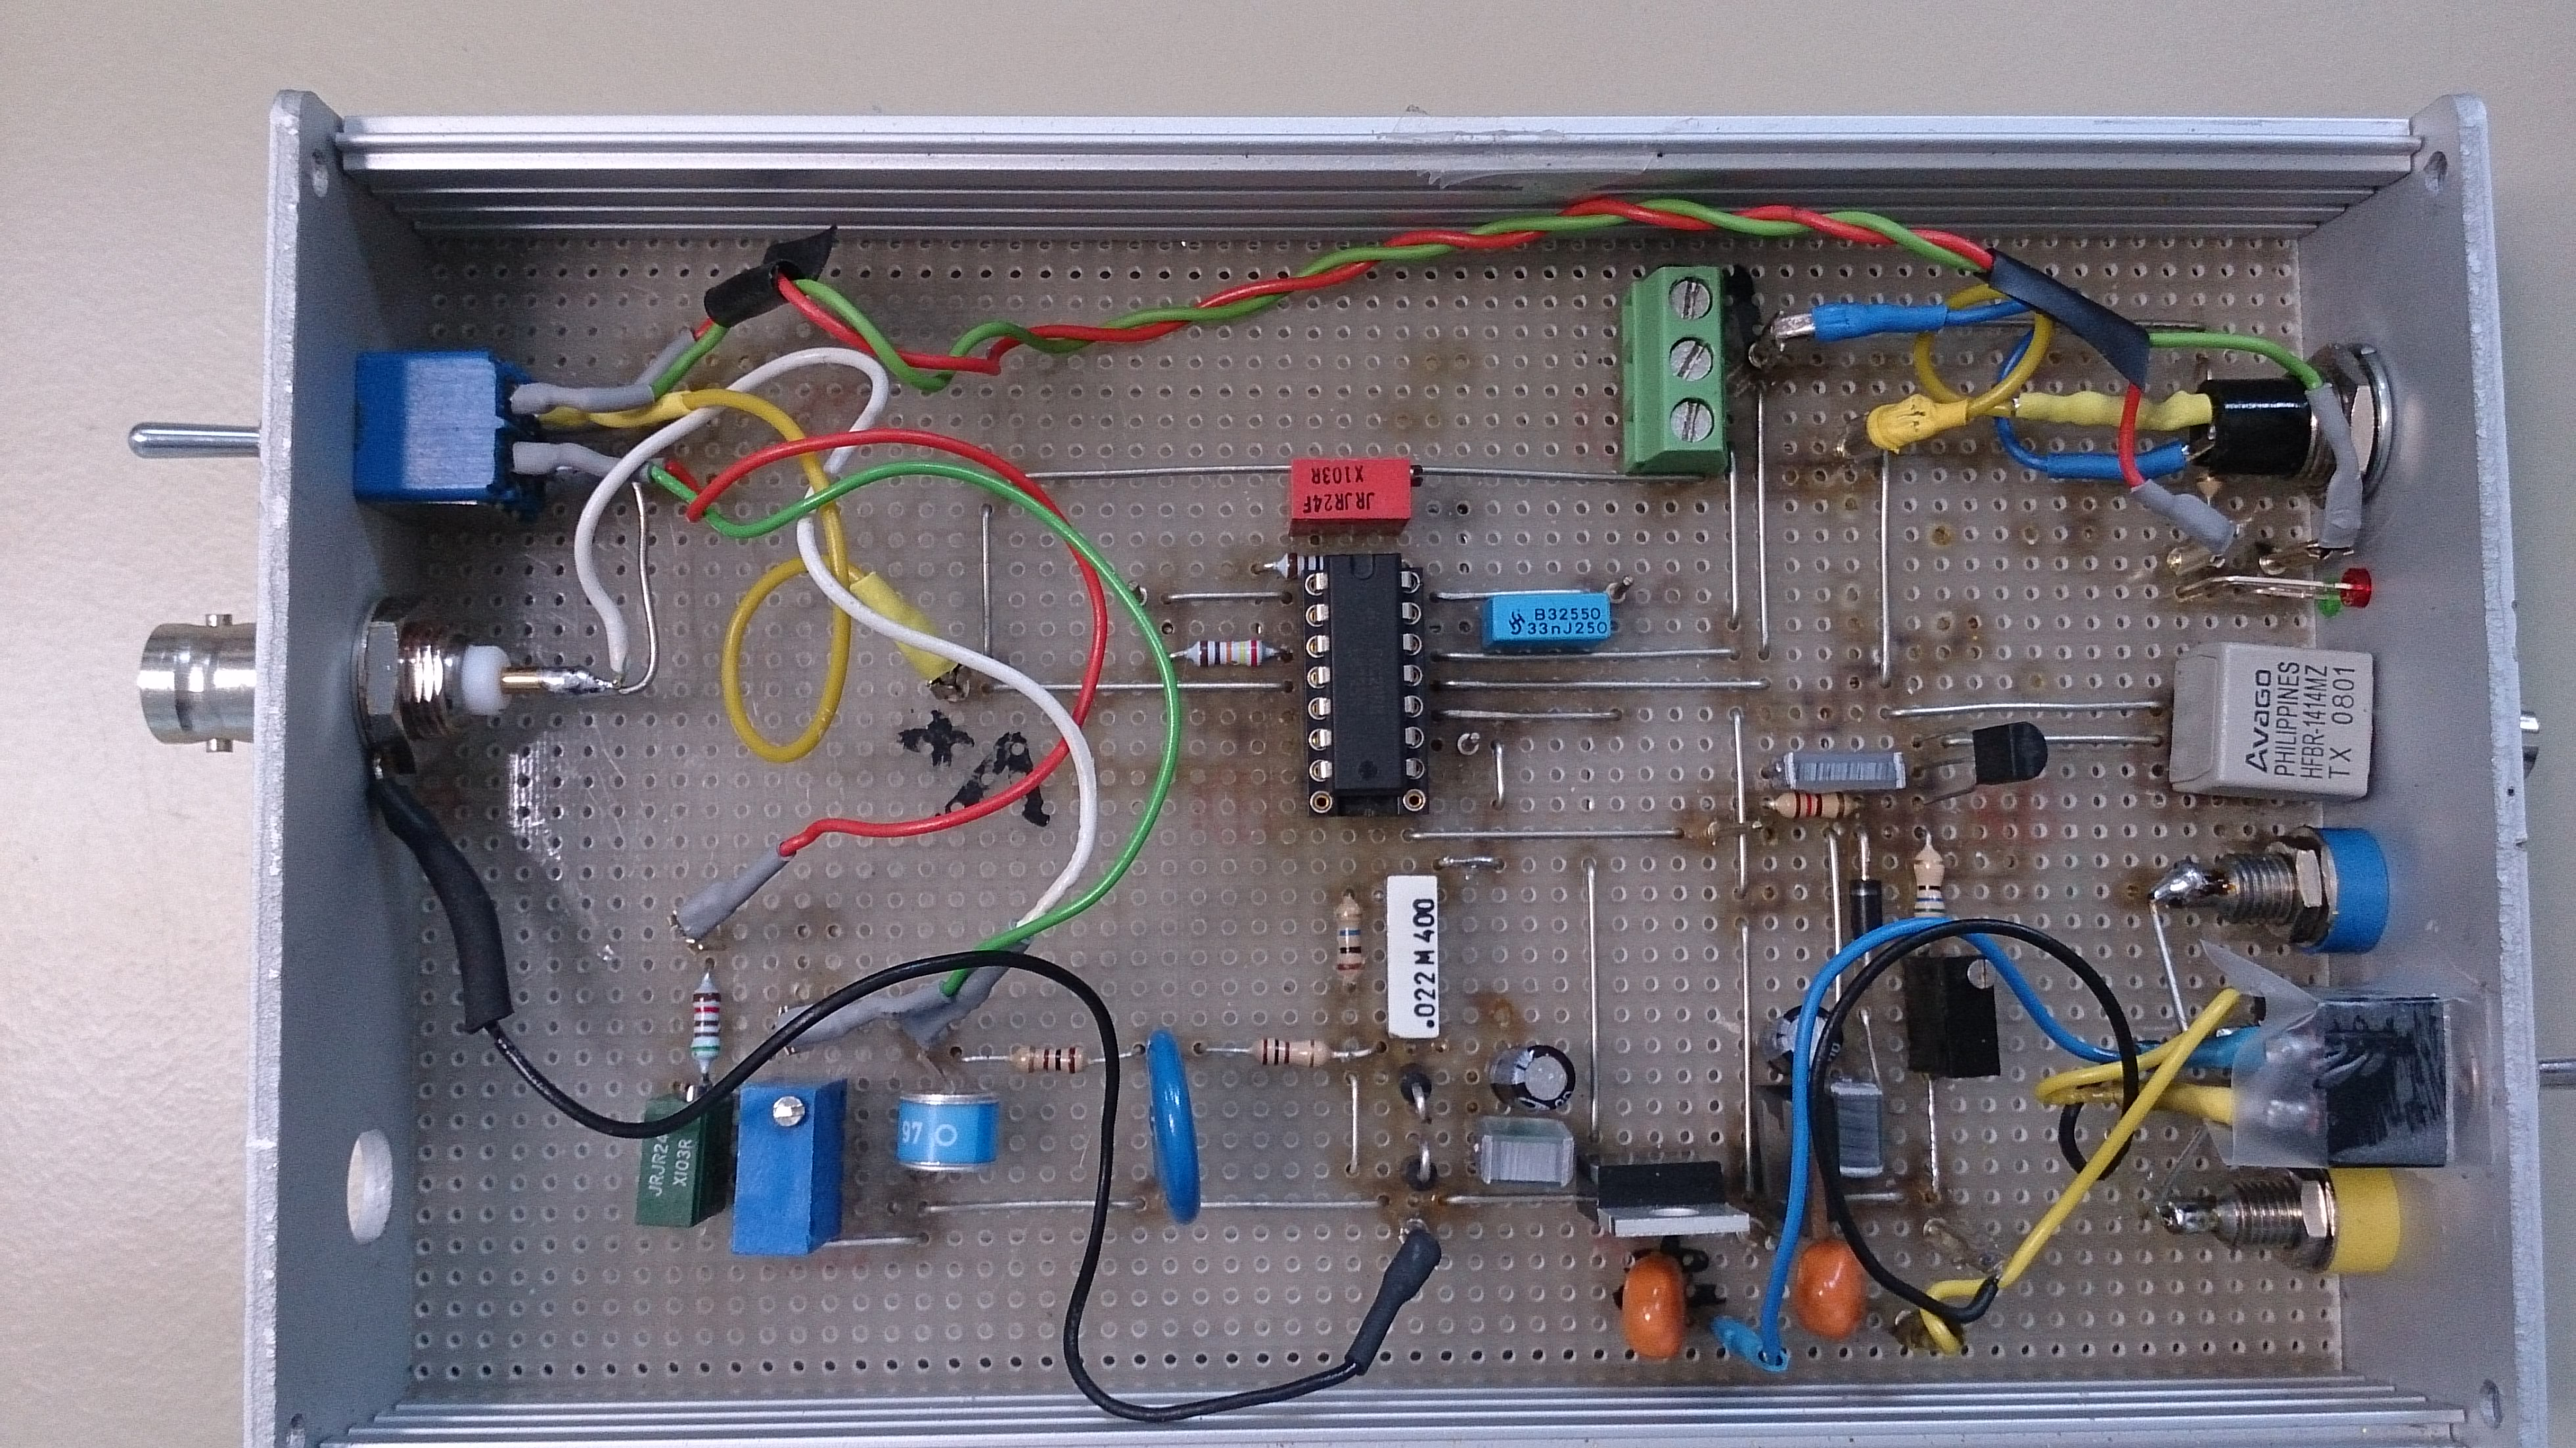
\includegraphics[scale=0.08]{gfx/inside/tx.JPG}
	\caption{Aufbau Sendeeinheit}
\end{figure}

\begin{figure}[H]
	\centering
	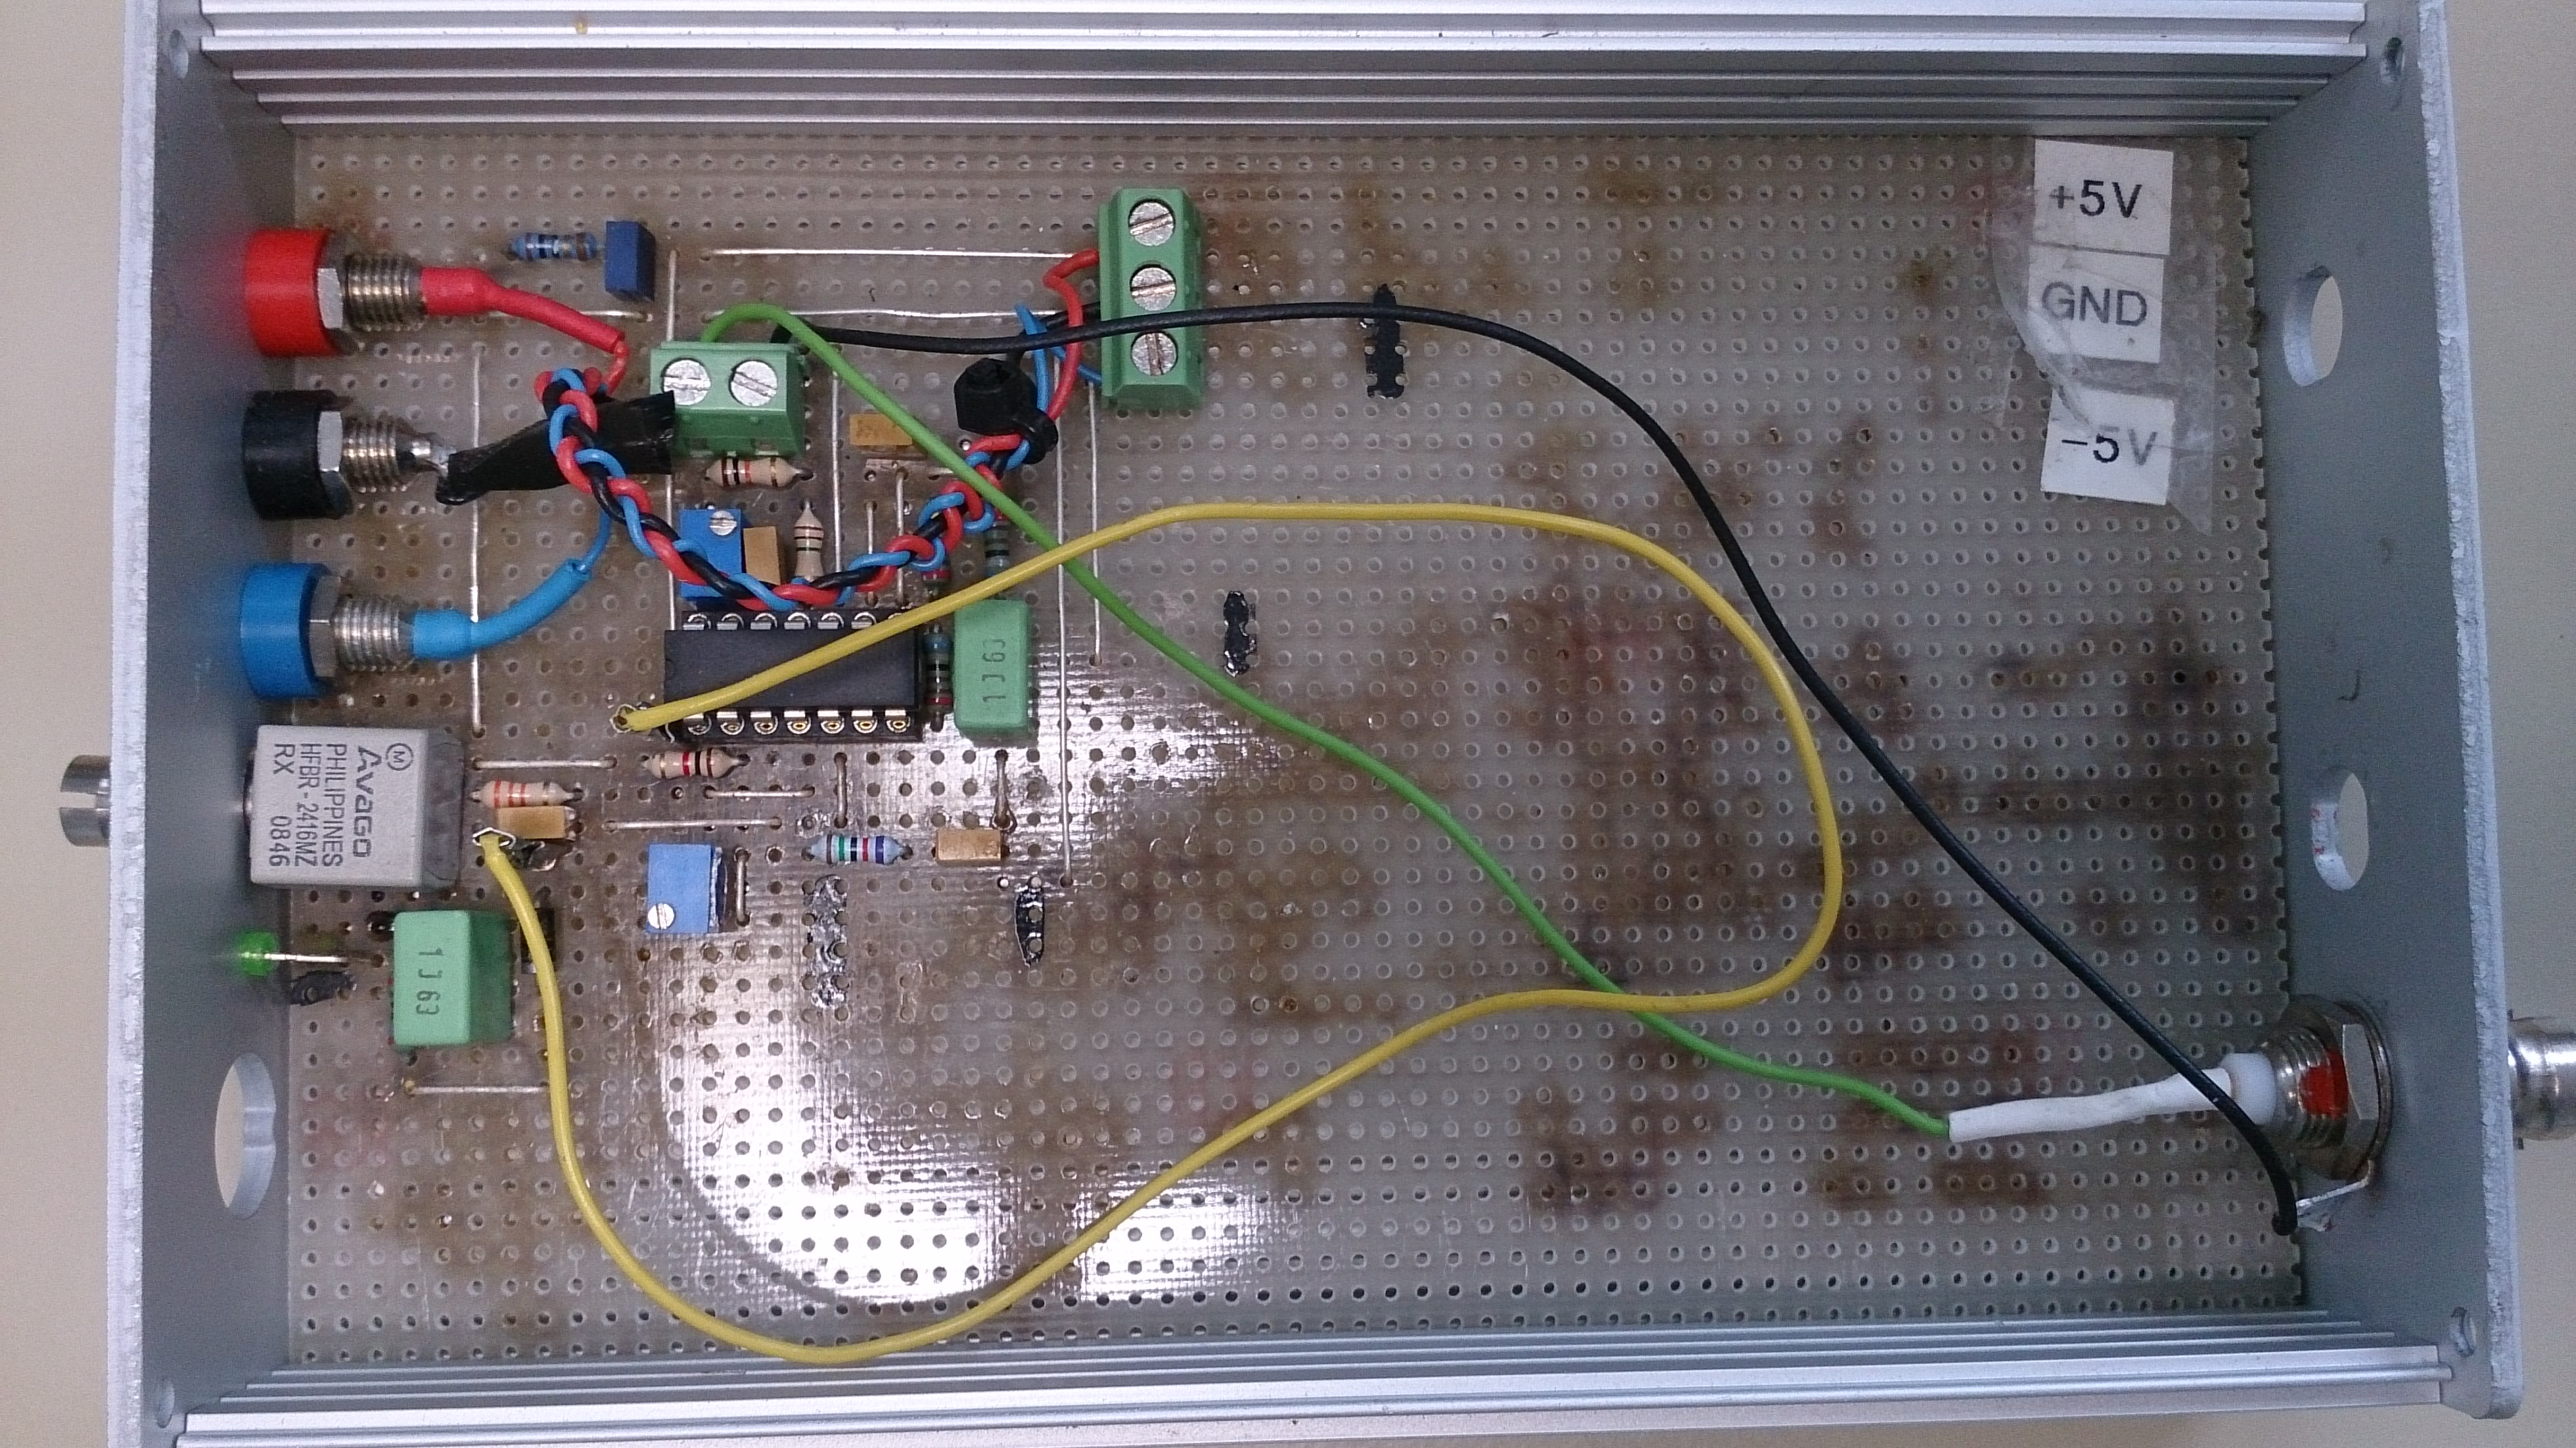
\includegraphics[scale=0.08]{gfx/inside/rx.JPG}
	\caption{Aufbau Empfangseinheit}
\end{figure}

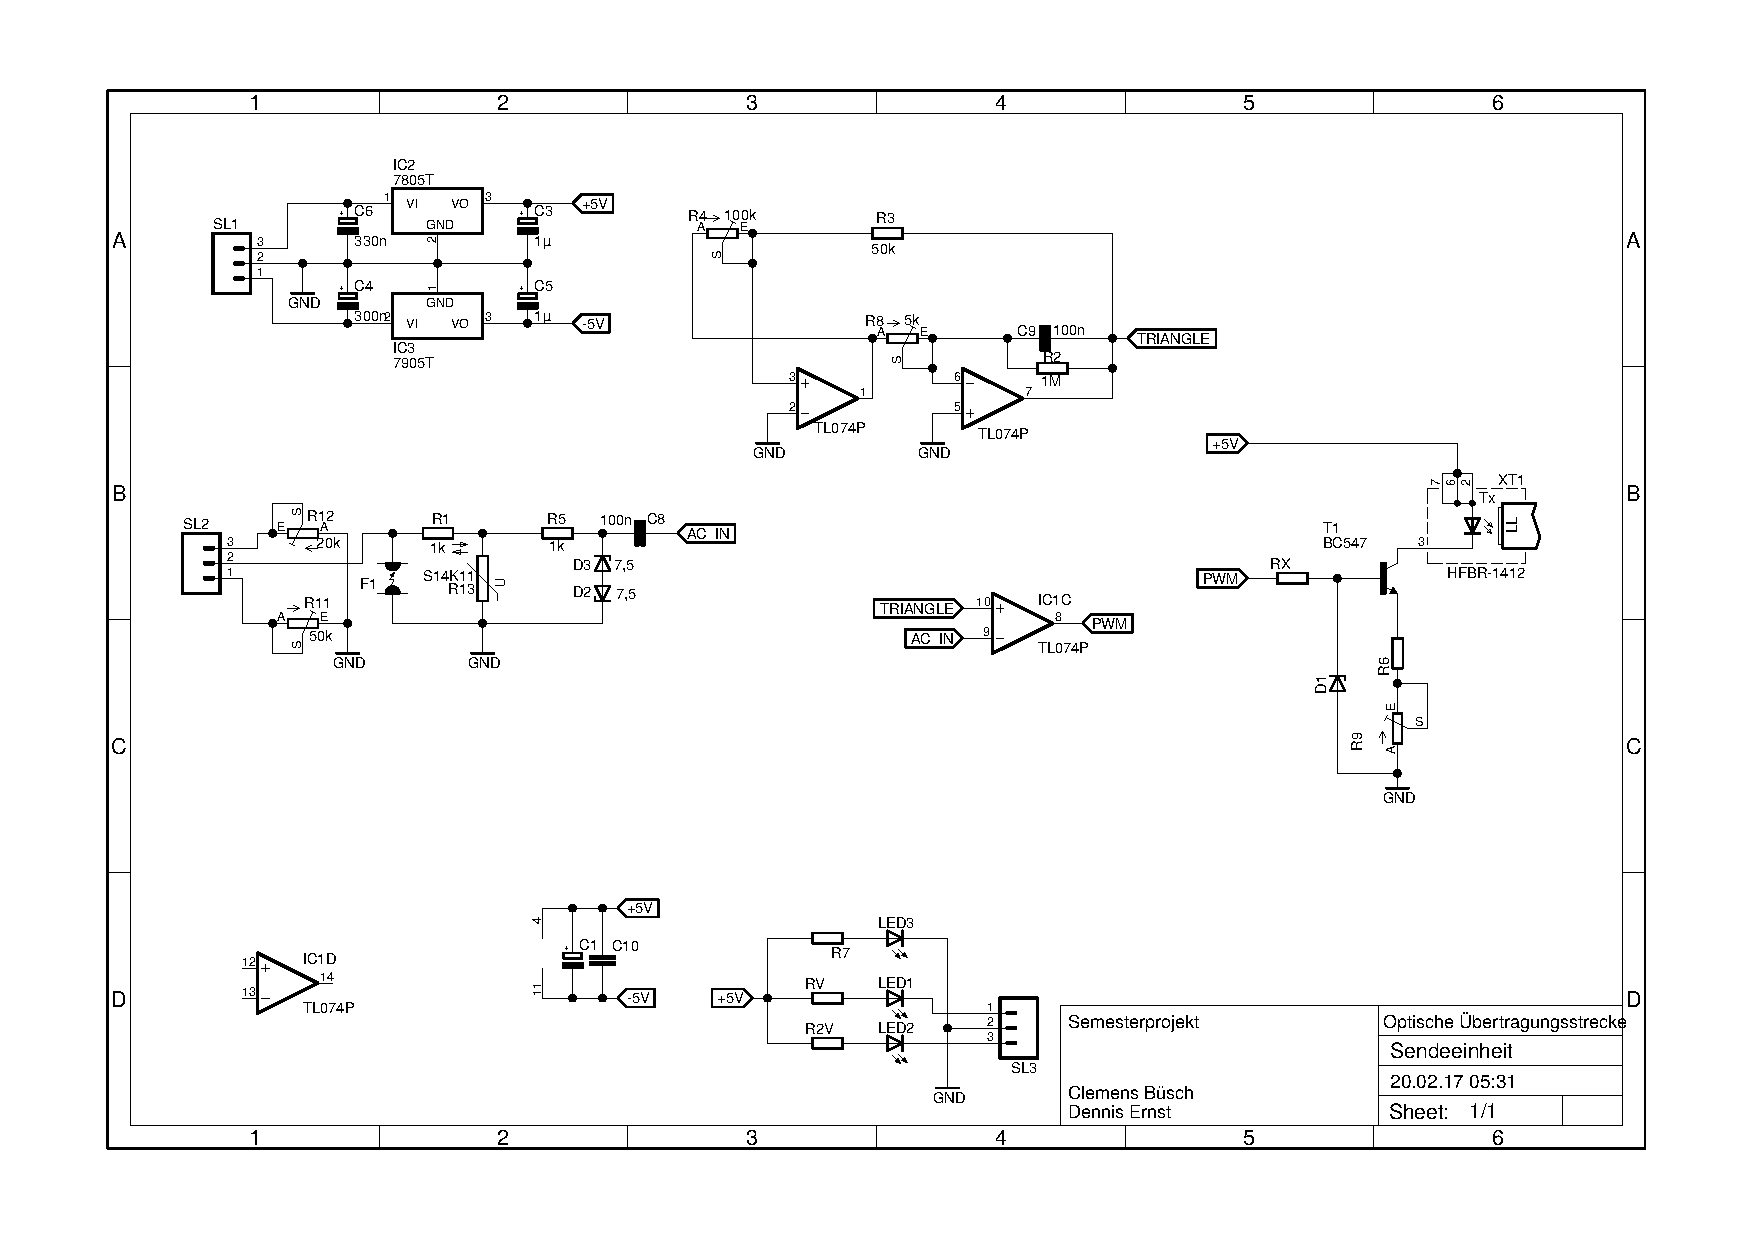
\includepdf[pages=1,angle=90]{gfx/TxSchematic.pdf}
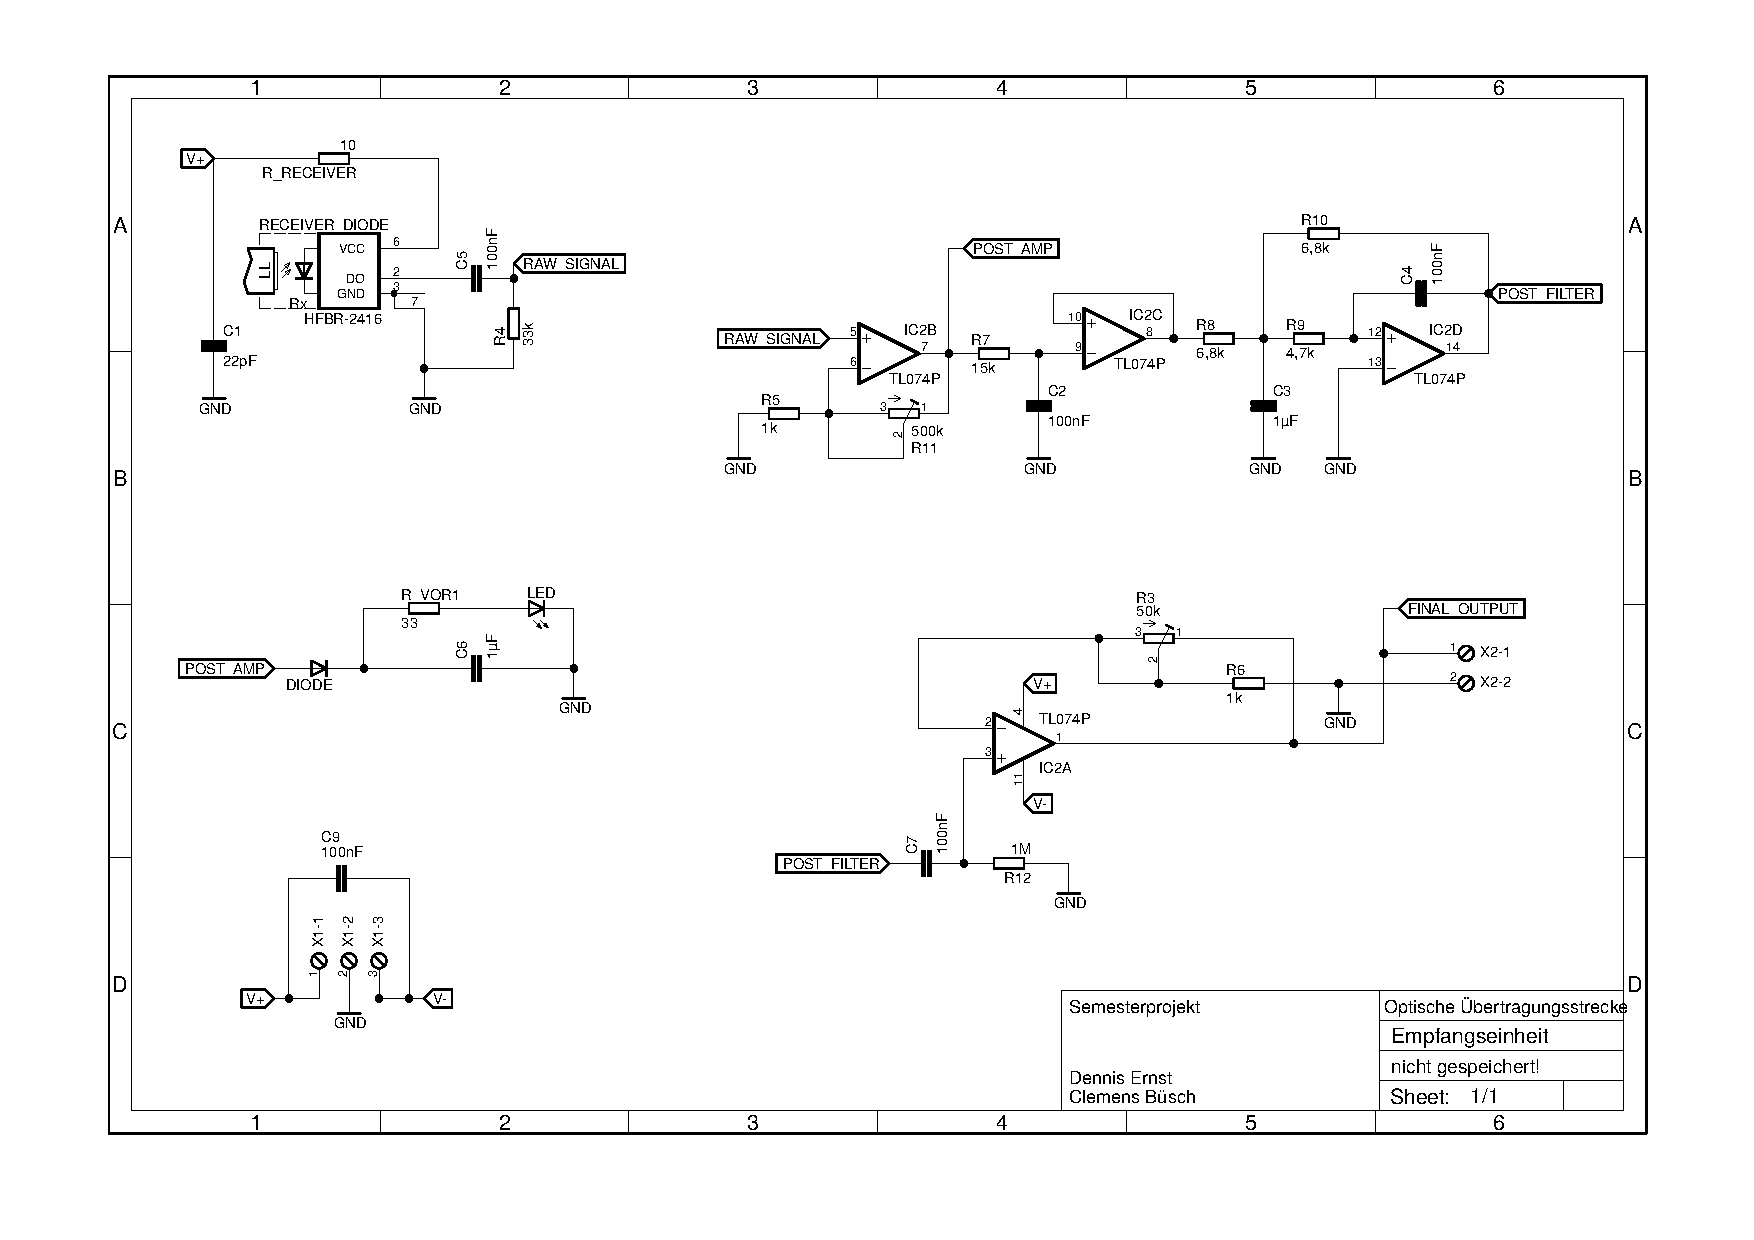
\includepdf[pages=1,angle=90]{gfx/RxSchematic.pdf}


\listoffigures




\end{document}
              